% This is my thesis, read it first and I will ask questions
% later also in comments. 

\documentclass[a4paper,12pt]{article}

\setlength{\textwidth}{15.0cm}
\setlength{\textheight}{24.0cm}
\setlength{\topmargin}{0cm}
\setlength{\headsep}{0cm}
\setlength{\headheight}{0cm}
\pagestyle{plain}


\usepackage{hyperref}
\hypersetup{
    colorlinks=true,
    linkcolor=blue,
    filecolor=magenta,      
    urlcolor=blue,
    citecolor=blue,
    linktoc=page
}
\usepackage[dvips]{epsfig}
\usepackage{tikz}
\usepackage[english]{babel}
\usepackage{caption}
\captionsetup{font=it}
\usepackage[autostyle, english=american]{csquotes}


\usepackage[
backend=biber,
style=alphabetic,
]{biblatex}

\renewcommand{\bibfont}{\footnotesize}


\usepackage{amsmath,amssymb,amsthm}
\newtheoremstyle{break}{4pt}{4pt}{}{}{\bfseries}{\vspace{2 pt}}{\newline}{}
\theoremstyle{break}
\newtheorem{theorem}{Theorem}[subsection]
\newtheorem{example}[theorem]{Example}
\newtheorem{definition}[theorem]{Definition}
\newtheorem{notation}[theorem]{Notation}
\newtheorem{lemma}[theorem]{Lemma}
\newtheorem{corollary}[theorem]{Corollary}
\newtheorem{technique}[theorem]{Technique}
\newtheorem{pythonn}[theorem]{Python Code}
\newtheorem{related}[theorem]{Related Work}

\usepackage{comment}
\usepackage{listings}
% Define custom colors for Python syntax highlighting
\definecolor{codebackground}{RGB}{242, 242, 242}
\definecolor{codecomment}{RGB}{106, 153, 85}
\definecolor{codekeyword}{RGB}{0, 0, 255}
\definecolor{codestring}{RGB}{170, 55, 241}

% Define custom Python style for syntax highlighting
\lstdefinestyle{custompython}{
    language=Python,
    backgroundcolor=\color{codebackground},
    basicstyle=\ttfamily\footnotesize,
    commentstyle=\color{codecomment}\itshape,
    keywordstyle=\color{codekeyword}\bfseries,
    stringstyle=\color{codestring},
    showstringspaces=false,
    breaklines=true,
    breakatwhitespace=true,
    tabsize=4,
    frame=tb,
    framesep=4pt,
    framerule=0.5pt,
    numbers=left,
    numbersep=10pt,
    numberstyle=\footnotesize\color{gray},
    xleftmargin=15pt,
    xrightmargin=5pt,
    aboveskip=5pt,
    belowskip=5pt,
    captionpos=b
}

\newcommand{\pythoncode}[1]{
    \hspace*{0cm}
    \vspace{-0.3cm}
    \lstinputlisting[style=custompython]{#1}}

% Define custom colors for Julia syntax highlighting
\definecolor{juliabackground}{RGB}{240, 230, 255} % Light purple background
\definecolor{juliacomment}{RGB}{128, 0, 128}     % Purple comments
\definecolor{juliakeyword}{RGB}{75, 0, 130}      % Indigo keywords
\definecolor{juliastring}{RGB}{147, 112, 219}    % Medium purple strings

% Define custom Julia style for syntax highlighting
\lstdefinelanguage{Julia}%
{
    morekeywords={
            abstract, break, case, catch, const, continue, do, else, elseif, end,
            export, false, for, function, global, if, immutable, import, importall,
            in, macro, module, otherwise, quote, return, switch, true, try, type,
            typealias, using, while
        },
    sensitive=true,
    alsoother={$},
    morecomment=[l]\#,
    morecomment=[n]{\#=}{=\#},
    morestring=[s]{"}{"},
    morestring=[s]{'}{'},
}[keywords,comments,strings]

\lstdefinestyle{customjulia}{
    language=Julia,
    backgroundcolor=\color{juliabackground},
    basicstyle=\ttfamily\footnotesize,
    commentstyle=\color{juliacomment}\itshape,
    keywordstyle=\color{juliakeyword}\bfseries,
    stringstyle=\color{juliastring},
    showstringspaces=false,
    breaklines=true,
    breakatwhitespace=true,
    tabsize=4,
    frame=tb,
    framesep=4pt,
    framerule=0.5pt,
    numbers=left,
    numbersep=10pt,
    numberstyle=\footnotesize\color{gray},
    xleftmargin=15pt,
    xrightmargin=5pt,
    aboveskip=5pt,
    belowskip=5pt,
    captionpos=b,
    columns=flexible,
    keepspaces=true
}

\newcommand{\juliacode}[1]{
    \hspace*{0cm}
    \vspace{-0.3cm}
    \lstinputlisting[style=customjulia]{#1}
}

\addbibresource{bibliography3.bib} 
\setlength{\parindent}{0pt}

\selectlanguage{English}
\begin{document}

\begin{titlepage}
    \begin{center}
        \resizebox{3cm}{!}{
\includegraphics{./vert2_kl_01.eps}}
        \ \
        \ \\
        \ \\
        \ \\
        \ \\
        \ \\
        \ \\
        \ \\
        \ \\
        \ \\
        \ \\
        \ \\
        \Large{M{\sc asterproef scriptie}}
        \ \\
        \ \\
        \ \\
        \huge{\bf{\em Recursive Monte Carlo for linear ODEs}}
        \ \\
        \ \\
        \ \\
        % \ \\
        \ \\
        \ \\
        \normalsize
        Auteur: {\em Isidoor Pinillo Esquivel}\\
        \ \\
        \ \\
        Promotor: {\em Wim Vanroose}\\
        \ \\
        \ \\
        \ \\
        \ \\
        \ \\
        \ \\
        \ \\
        A{\sc cademiejaar 2022-2023}

    \end{center}
\end{titlepage}




\newpage
\tableofcontents
\newpage

\begin{abstract}
  Unbiased algorithms for solving linear initial value problems have received limited attention.
This is addressed here by proposing unbiased Recursive Monte Carlo methods for solving
linear initial value problems and linear Fredholm integral equations of the second kind. Motivated
by understanding randomized parallel complexity and downstream applications to partial differential
equations, these methods are developed.

Previously only biased methods were known to achieve optimal convergence rates for nonlinear
initial value problems which has primarily theoretical significance.
The proposed RRMC method, an unbiased algorithm for linear initial value problems,
together with control variates is conjectured to be order optimal with high
probability for corresponding smoothness classes.

Parallel to this, the main Poisson algorithm is proposed, generalizing the algorithm in \cite{acebron_monte_2016},
which is simple and forward implementable. The main Poisson algorithm is applied
to the semi-discretized heat equation demonstrating a path resampling technique, that provides
a novel perspective on the Walk on Spheres method, with potential for alternative generalizations.

The proposed methods broadens the understanding of what is possible with unbiased algorithms for
solving linear initial value problems, paving the way for further research in this area.
\end{abstract}


\section{Introduction}

\subsection{Related Work}
The primary motivating paper for this work is the work
by \citeauthor{sawhney_grid-free_2022}
(\citeyear{sawhney_grid-free_2022}) \cite{sawhney_grid-free_2022},
which introduces the Walk-on-Sphere (WoS) method for solving second-order
elliptic PDEs with varying coefficients and Dirichlet boundary conditions.
Their techniques have shown high accuracy even in the presence of geometrically
complex boundary conditions. We were inspired to apply the underlying
mechanics of these Monte Carlo (MC) techniques to IVPs to explore
parallel in time and the possibility of extending their techniques
to other types of PDEs. \\

We made an interactive data map of the literature read
mainly in the function of this thesis available at
\url{https://huggingface.co/spaces/ISIPINK/zotero_map}.\\

Existing randomized algorithms for solving IVPs in general are either based
on MC integration or randomizing parts of deterministic
algorithms. Typically motivated by lower smoothness conditions where
randomization adds significant
convergence speed or solving ODEs where randomization
aids in parallelization .\\

\citeauthor{daun_randomized_2011}'s \citeyear{daun_randomized_2011}
\cite{daun_randomized_2011} proposes a biased algorithm that has optimal Information-Based
Complexity (IBC) for some smoothness classes. Similarly to us, their method uses control variates.\\


\citeauthor{ermakov_monte_2021}'s \citeyear{ermakov_monte_2021}
\cite{ermakov_monte_2021} proposes an unbiased method for
a Cauchy problem for large systems of linear ODEs.
Similarly to us, their method is based on Volterra integral equations.\\

\section{Background}

\subsection{Monte Carlo Integration}

In this subsection, we review basic MC theory. \\

\begin{notation}[Random Variables]
  Random variables (RVs) will be denoted with capital letters, e.g., $X$, $Y$ or $Z$.
\end{notation}


MC integration is any method that involves random sampling to
estimate an integral.
\begin{definition}[Uniform Monte Carlo Integration]
  We define uniform MC integration of
  $f:\mathbb{R} \rightarrow \mathbb{R}$
  over $[0,1]$ as
  an estimation of the expected value of $f(U)$, with
  $U \sim \text{Uniform}(0,1)$. Combined
  with the Best Linear Unbiased Estimators (BLUEs), MC Integration
  in that case, can be summarized in the following formula:
  \begin{equation}\label{eq:BLUE}
    \int_{0}^1 f(s)ds \approx \frac{1}{n} \sum_{j=1}^{n}f(U_{j}),
  \end{equation}
  \juliacode{julia_code/uniform_MC.jl}
  where $n$ is the amount of samples used and $U_{j}$ i.i.d. $\text{Uniform}(0,1)$.
\end{definition}

Because estimators are random variables (RVs), the cost and error are also random
variables. In most cases, obtaining these RVs is difficult to impossible.
Directly comparing estimators based on these RVs can be challenging;
there is no simple Pareto front. Instead, comparisons can be made
using statistics. \\

Accuracy comparisons between estimators
are typically conducted with (root-)mean-square error (RMSE).
\begin{definition}[Root-Mean-Square Error]
  We define the Root-Mean-Square Error (RMSE) of an estimator $\tilde{\theta}$ for $\theta$  as follows:
  \begin{equation}
    \text{RMSE}(\tilde{\theta}) = \sqrt{E[||\tilde{\theta}-\theta||^{2}_{2}]}.
  \end{equation}
\end{definition}

Even comparisons based on RMSE can be counterintuitive; consider Stein's paradox,
for example. We limit ourselves to simple cases such as $1$-dimensional
unbiased estimators, making MSE equivalent to variance.
Estimating variance is most cases possible and can be used to calculate
confidence intervals using Chebyshev's inequality.\\

Average floating point operations or time per simulation are common cost statistics.
It may also be useful to consider \enquote*{at risk}  (analogous to \enquote*{value at risk})
in terms of memory or wall time.

If we limit ourselves to (\ref{eq:BLUE}) with a big sample size and
finite variance assumption on error and simulation time,
simulations can be computed in parallel, making them well-suited for a GPU implementation.
These assumptions are useful for establishing a baseline and
when they are close to being optimal, they become highly practical.
In this case, there is a linear trade-off
between average simulation time and variance which motivate
the definition of MC efficiency for comparing estimators.

\begin{definition}[Monte Carlo Efficiency]
  Define MC efficiency of an
  estimator $F$ as follows:
  \begin{equation}
    \epsilon[F]=\frac{1}{\text{Var}(F) T(F)},
  \end{equation}
  with $T$ the average simulation time.
\end{definition}

\begin{related}[Monte Carlo Efficiency]
  For a reference see \cite{veach_robust_1997} page 45.
\end{related}

For smooth $1$-dimensional integration, the linear trade-off between
variance and average simulation time is not even close to optimal see
Theorem \ref{thrm:order trap}. \\
When it comes to comparing better trade-offs,
Information-Based Complexity (IBC) is often employed.
IBC primarily serves as a
qualitative measure and does not necessarily imply the
practicality of an algorithm. We will not delve into a
rigorous definition of IBC.

\begin{definition}[Information-Based Complexity]
  IBC is a way to describe asymptotically (for increasing accuracy/function calls)
  the trade-off between the average amount of function calls (information)
  needed and accuracy.
\end{definition}

\begin{example}[IBC of (\ref{eq:BLUE})]
  In (\ref{eq:BLUE}) the function calls trades of
  linearly with variance. For $n$ function calls,
  the RMSE $= O\left(\frac{1}{\sqrt{n}}\right)$ or equivalently, if we want a
  RMSE of $\varepsilon$ we would need $O\left(\frac{1}{\varepsilon^{2}}\right)$
  function calls.
\end{example}


\subsection{Recursive Monte Carlo}
In this subsection, we introduce Recursive Monte Carlo (RMC)
with the following  initial value problem:


\begin{equation} \label{ydy}
  y_t = y, \quad y(0) = 1.
\end{equation}


By integrating both sides of (\ref{ydy}), we obtain:

\begin{equation} \label{Integral ydy}
  y(t) = 1 + \int_{0}^{t} y(s) ds.
\end{equation}

(\ref{Integral ydy}) represents a recursive integral equation,
specifically, a linear Volterra integral equation of the second type.

\begin{notation}[$U,U_{j}$]
  We will frequently use the uniform distribution, so we will abbreviate it
  \begin{equation}
    U_{j}  \text{ i.i.d Uniform}(0,1).
  \end{equation}

  The subscripts are used to clarify independence
  between uniforms. However,
  when there is no risk of confusion,
  we simply use $U.$
\end{notation}

By estimating the recursive integral in (\ref{Integral ydy})
using MC, we derive the following estimator:

\begin{equation}
  Y(t) = 1 + t  y(Ut).
\end{equation}


If $y$ is well-behaved, then $E[Y(t)] = y(t)$.
However, we cannot directly simulate $Y(t)$ without access
to $y(s)$ for $s < t$. Nevertheless, we can replace $y$ with
an unbiased estimator without affecting $E[Y(t)] = y(t)$,
by the law of total expectation ($E[X] = E[E[X|Z]]$).
By replacing $y$ with $Y$ itself, we obtain a recursive
expression for $Y$:

\begin{equation} \label{recursive RV}
  Y(t) = 1 + t  Y(Ut).
\end{equation}

\juliacode{julia_code/RMC_example.jl}

(\ref{recursive RV}) is a Recursive Random Variable
Equation (RRVE).

\begin{definition}[Recursive Random Variable
    Equation (RRVE)]
  A Recursive Random Variable Equation (RRVE) is
  an equation that defines a
  family of random variables in terms of itself.
\end{definition}

Simulation of $Y$ with (\ref{recursive RV}),
would recurse indefinitely (every $Y$ needs to sample another $Y$).
To stop the recursion, approximate
$Y(t) \approx 1$ near $t = 0$ introducing minimal bias.
Later, we will discuss Russian roulette; see Definition \ref{Russian roulette},
which can be used as an unbiased stopping mechanism.

\subsection{Modifying Monte Carlo}

In this subsection, we discuss techniques for modifying RRVEs
in a way that preserves the expected value of the solution while
acquiring more desirable properties. These techniques are only
effective when applied by using prior information
about the problem or computational costs. \\

We will frequently interchange RVs with the same expected values.
Therefore introduce following notation:
\begin{notation}[$\cong$]
  \[
    X \cong Y \iff E[X]=E[Y]
    .\]
\end{notation}

Russian roulette is a MC technique commonly employed in rendering algorithms.
The concept behind Russian roulette is to replace an RV with a
less computationally expensive approximation sometimes.

\begin{definition}[Russian roulette] \label{Russian roulette}
  We define Russian roulette on $X$ with free parameters
  $Y_{1} \cong Y_{2}$, $p \in [0,1]$
  and $U$ independent of $Y_{1}$, $Y_{2}$, $X$
  as follows:

  \begin{equation}
    X \cong
    \begin{cases}
      \frac{1}{p}(X - (1-p)Y_{1}) & \text{ if } U < p \\
      Y_{2}                       & \text{ else }
    \end{cases}.
  \end{equation}
\end{definition}


\begin{notation}[$B(p)$]
  Often Russian roulette will be used with $Y_{1}= Y_{2}= 0$.
  In that case, we use Bernoulli variables to shorten notation.
  \begin{equation}
    B(p) \sim \text{Bernoulli}(p) =
    \begin{cases}
      1 & \text{ if } U<p \\
      0 & \text{ else }
    \end{cases} .
  \end{equation}
\end{notation}

\begin{example}[Russian roulette] \label{ex:simple russian roulette}
  Consider the estimation of $E[Z]$, with $Z$:

  \begin{equation}
    Z = U + \frac{f(U)}{1000}.
  \end{equation}

  Here, $f:\mathbb{R} \rightarrow [0,1]$ is expensive to compute.
  Directly estimating $E[Z]$ would involve evaluating $f$ for each sample which
  contributes little to the accuracy.
  To address this, we can modify $Z$ to:

  \begin{equation}
    Z \cong U + B\left(\frac{1}{100}\right)\frac{f(U)}{10}.
  \end{equation}

  This requires calling $f$ on
  average once every $100$ samples. This significantly reduces the
  computational burden while increasing the variance slightly thereby increasing
  the overall MC efficiency.\\
\end{example}

\begin{related}[Example \ref{ex:simple russian roulette}]
  In Example \ref{ex:simple russian roulette}, it is also
  possible to estimate the expectations of the $2$ terms
  of $Z$ separately. Given the variances and computational costs
  of both terms, you can calculate the asymptotically optimal division
  of samples for each term. However, this is no longer the case with RMC.
  In \cite{rath_ears_2022}, a method is presented to estimate the optimal
  Russian roulette/splitting factors for rendering.
\end{related}


\begin{example}[Russian roulette on (\ref{recursive RV})] \label{ex: russian roulette}
  To address the issue of indefinite recursion in
  (\ref{recursive RV}), Russian roulette can be employed
  by approximating the value of $Y$ near $t = 0$ with $1$
  sometimes. Specifically, we replace the coefficient $t$
  in front of the recursive term with $B(t)$ when $t < 1$.
  The modified recursive expression for $Y(t)$ for $t<1$ becomes:

  \begin{equation}\label{eq:rr example}
    y(t) \cong Y(t) = 1 + B(t)Y(Ut)
  \end{equation}
  \juliacode{julia_code/RR_example.jl}

  Interestingly, $\forall t \le 1:Y(t)$ is the number of recursion calls
  to sample $Y(t)$ such that the average number of recursion
  calls to sample $Y(t)$ equals $e^{t}$.

\end{example}

Splitting is a technique that increases samples of important terms, similar to how Russian roulette
decreases the samples of unimportant terms.

\begin{definition}[splitting] \label{def:splitting}
  Splitting $X$ refers to utilizing multiple $X_{j} \cong X$ (not necessarily independent) to
  reduce variance by taking their average:
  \begin{equation}
    X \cong \frac{1}{N} \sum_{j=1}^{N} X_{j}.
  \end{equation}
\end{definition}

Splitting the recursive term in an RRVE can result in additive branching recursion,
necessitating cautious management of terminating the branches promptly to prevent
exponential growth in computational complexity. To accomplish this, termination
strategies that have been previously discussed can be employed. Subsequently,
we will explore the utilization of coupled recursion as a technique to mitigate
additive branching recursion in RRVEs (see Example \ref{ex:coupled splitting}).

\begin{example}[splitting on (\ref{eq:rr example})] \label{ex:splitting}
  We can "split" the recursive term of (\ref{eq:rr example})
  into two parts as follows:

  \begin{equation}\label{eq:splitting}
    y(t) \cong Y(t) =1 + \frac{B(t)}{2}(Y_{1}(U_{1}t) + Y_{2}(U_{1}t))
  \end{equation}

  \juliacode{julia_code/split_example1.jl}

  \begin{equation}\label{eq:splitting2}
    y(t) \cong Y(t) =1 + \frac{B(t)}{2}(Y_{1}(U_{1}t) + Y_{2}(U_{2}t))
  \end{equation}

  \juliacode{julia_code/split_example2.jl}

  where $Y_{1}(t)$ and $Y_{2}(t)$ are i.i.d. with $Y(t)$.
\end{example}

\begin{definition}[control variates] \label{CV}
  Define control variating $f(U)$ with $\tilde{f}$ an approximation of $f$ as:

  \begin{align}
    f(U) & \cong f(U_{1})-\tilde{f}(U_{1}) + E[\tilde{f}(U)] \\
         & = (f-\tilde{f})(U_{1}) + E[\tilde{f}(U)]
    .
  \end{align}

  Note that control variating requires the evaluation of
  $E[\tilde{f}(U)]$.  When this is estimated instead, we refer to it as $2$-level MC
  and recursively applying $2$-level is multilevel MC.
\end{definition}


\begin{example}[control variate on (\ref{recursive RV})] \label{ex:CV}
  To create a control variate for (\ref{recursive RV}) that
  effectively reduces variance, we employ the approximation
  $y(t) \approx \tilde{y} =1+t$ and define the modified recursive term as follows:

  \begin{align}
    y(t) \cong Y(t) & = 1 + t(Y(U_{1}t) - \tilde{y}(U_{1}t) + E[\tilde{y}(Ut)])     \\
                    & = 1 + t \left( E[1 + Ut]  \right) + t(Y(U_{1}t) - 1 - U_{1}t) \\
                    & = 1 + t + \frac{t^2}{2} + t(Y(U_{1}t) - 1 - U_{1}t).
  \end{align}
  \juliacode{julia_code/CV_example.jl}

  Note that while we could cancel out the constant term
  of the control variate, doing so would have a negative impact
  on the Russian roulette implemented.
\end{example}

\begin{related}[MC modification]
  For further reference on Russian roulette, splitting and control variates
  see \cite{veach_robust_1997}.
\end{related}

\subsection{Monte Carlo Trapezoidal Rule}

In this subsection, we introduce an MC trapezoidal rule that
exhibits similar convergence behavior to the methods discussed later.
The MC trapezoidal rule is essentially a regular Monte Carlo method
enhanced with control variates based on the trapezoidal rule.

\begin{definition}[MC trapezoidal rule]
  We define the MC trapezoidal rule for approximating the integral
  of function $f$ over the interval $[x, x+\Delta x]$ with a Russian roulette rate
  $l$ and $\tilde{f}$ represents the linear approximation of $f$ corresponding
  to the trapezoidal rule as follows:

  \begin{align}
     & \int_{x}^{x+\Delta x} f(s) ds                           \\
     & = \int_{x}^{x+\Delta x}  \tilde{f}(s) ds +
    \int_{x}^{x+\Delta x}  f(s) - \tilde{f}(s) ds              \\
     & = \Delta x \frac{f(x) + f(x+\Delta x)}{2}
    + E \left[f(S) - \tilde{f}(S)\right]                       \\
     & \cong \Delta x \frac{f(x) + f(x+\Delta x)}{2} \nonumber \\
     & + \Delta x l B\left( \frac{1}{l}\right)
    \left(f(S) - f(x) - \frac{S - x}{\Delta x}
    \left(f(x+\Delta x) - f(x)\right) \right), \label{eq:MCtrap}
  \end{align}

  where $S \sim \text{Uniform}(x,x+\Delta x)$.
\end{definition}

\begin{lemma}[RMSE MC Trapezoidal Rule] \label{lem:rmse mctrap}
  The MC trapezoidal rule
  for a twice differentiable function has
  \begin{equation}
    \text{RMSE} =O\left( \Delta x^{3} \right) .
  \end{equation}
\end{lemma}

\begin{proof}
  Start from (\ref{eq:MCtrap}). The MSE is the variance
  so we can ignore addition by constants.

  \begin{equation}
    \text{MSE} = \text{Var}\left( \Delta x l B\left( \frac{1}{l}\right)
    \left(f(S) - f(x) - \frac{S - x}{\Delta x}
    \left(f(x+\Delta x) - f(x)\right) \right)\right)
  \end{equation}
  We substitute $S = \Delta x U + x$ and apply Taylor's theorem
  finishing the proof:

  \begin{align}
    \text{MSE} & = \text{Var}\left( \Delta x l B\left( \frac{1}{l}\right)
    \left(f(\Delta x U+x) - f(x) - U
    \left(f(x+\Delta x) - f(x)\right) \right)\right)                           \\
               & = \text{Var}\left( \Delta x l B\left( \frac{1}{l}\right)
    \left( U \Delta x f'(x)+ \frac{U^{2} \Delta x ^{2}}{2} f''(Z_{1})
    - U \left( \Delta x f'(x) +
    \Delta x ^{2} f''(z_{2})\right) \right)\right)                             \\
               & = \text{Var}\left( \Delta x l B\left( \frac{1}{l}\right)
    \left( \frac{U^{2} \Delta x ^{2}}{2} f''(Z_{1})
    -  \frac{U\Delta x ^{2}}{2} f''(z_{2}) \right)\right)                      \\
               & =\Delta x ^{6} \text{Var}\left(  l B\left( \frac{1}{l}\right)
    \left( \frac{U^{2} }{2} f''(Z_{1})
    -  \frac{U}{2} f''(z_{2}) \right)\right),
  \end{align}
  for some $Z_{1} \in [x,S], z_{2} \in [x,x+\Delta x]$. The variance term is bounded
  because the variance of a bounded RV is bounded.
  Note that the proof does not rely on Russian roulette ($l=1$).
\end{proof}

\begin{related}[proof of Lemma \ref{lem:rmse mctrap}]
  A more generalizable proof for other types of control variates can
  be constructed by applying the \enquote*{separation of the main part} technique,
  as shown in Lemma 4 of \cite{heinrich_monte_1993}.
\end{related}


\begin{definition}[composite (MC) trapezoidal rule] \label{MCtrap}
  Define the MC trapezoidal rule for approximating the integral
  of function $f$ over the interval $[0, 1]$ with a uniform grid
  with $n$ intervals as follows:

  \begin{equation}
    \int_{0}^{1} f(s) ds \approx \Delta x \sum_{j=0}^{n-1}  \frac{f(x_{j}) + f(x_{j}+\Delta x)}{2} .
  \end{equation}
  \juliacode{julia_code/composite_trapezoidal.jl}

  Define the  corresponding composite MC trapezoidal
  with a Russian roulette rate $l$ as follows:

  \begin{align} \label{eq:cMCtrap}
    \int_{0}^{1} f(s) ds \cong \Delta x \sum_{j=0}^{n-1} & \frac{f(x_{j}) + f(x_{j}+\Delta x)}{2} \nonumber \\
                                                         & + l B\left(\frac{1}{l}\right)
    \left(f(S_j) - f(x_{j}) - \frac{S_j - x_{j}}{\Delta x}(f(x_{j}+\Delta x) - f(x_{j}))\right),
  \end{align}

  \juliacode{julia_code/MC_composite_trapezoidal.jl}

  where $S_j \sim \text{Uniform}(x,x+\Delta x)$.

\end{definition}

% \begin{pythonn}[implementation of (\ref{eq:cMCtrap})]
%     We implement (\ref{eq:cMCtrap}) for $\int_{0}^{1}e^{s}ds$.
%     \vspace*{0.5cm}
%     \pythoncode{python code/trap1.py}

% \end{pythonn}

\begin{figure}[h!]
  \centering
  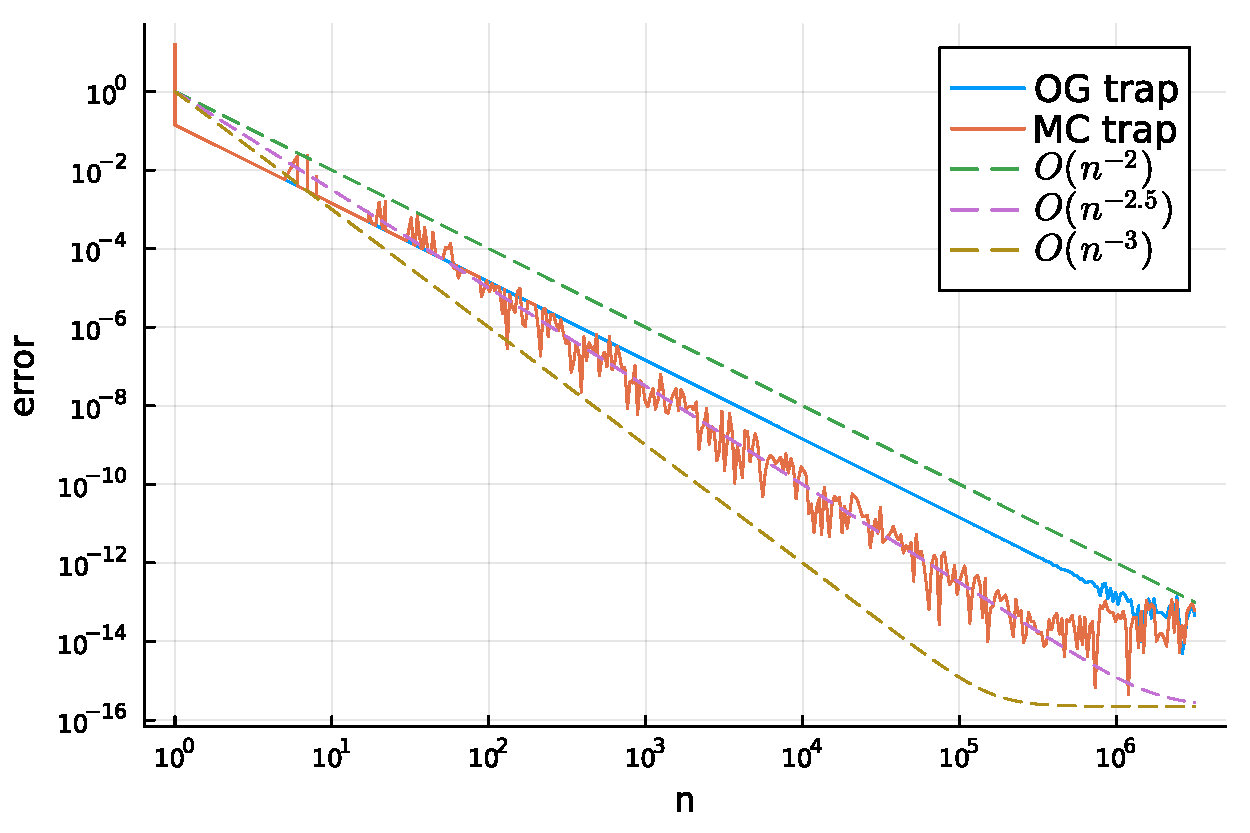
\includegraphics[width=0.8\textwidth]{julia_plots/trap_example.pdf}
  \caption{Log-log plot of the error of (\ref{eq:cMCtrap}) for
  $\int_{0}^{1}e^{s}ds$ with $l=100$. At floating point accuracy,
  the convergence ceases.
  }
  \label{fig:MCtrap}
\end{figure}

Figure \ref{fig:MCtrap} suggests that the order of convergence of RMSE of the
composite MC trapezoidal rule is better by $0.5$ than the normal composite trapezoidal rule.
The MC trapezoidal rule has on average $\frac{1}{l}$ more function calls than
the normal trapezoidal rule. For the composite rule with $n$ intervals,
there are $\text{Binomial}(n,\frac{1}{l})$ additional function calls
(repeated Bernoulli experiments).\\

\begin{theorem}[RMSE Composite Trapezoidal MC Rule] \label{thrm:order trap}
  The composite trapezoidal MC rule  with $n$ intervals
  for a twice differentiable function has
  \begin{equation}
    \text{RMSE} =O\left(\frac{1}{n^{2.5}} \right) .
  \end{equation}
\end{theorem}

The proof uses Lemma \ref{lem:rmse mctrap},
and is similar to the proof of the normal
trapezoidal rule. The main difference is the
accumulation of \enquote*{local truncation} errors into \enquote*{global truncation} error.
Normally there is a loss of one order but the MC trapezoidal loses only a half order
because the accumulation happens in variance instead of bias.

\begin{align}
  \sqrt{\text{Var}\left(\sum_{j=1}^{n}  \Delta x^{3}U_{j}^{2}\right)}
   & = \Delta x^{3} \sqrt{ \sum_{j=1}^{n}\text{Var} (U_{j}^{2})} \\
   & = \Delta x^{3} \sqrt{ n \text{Var}(U^{2})}                  \\
   & = O( \Delta x^{2.5}).
\end{align}

Note that the meaning of a bound on the error, which behaves as $O(\Delta x^{2})$,
and a bound on the RMSE, also behaving as $O(\Delta x^{2})$, is different.
A bound on the error implies a bound on the RMSE, but not vice versa.

\begin{related}[Monte Carlo Trapezoidal Rule]
  Due to an argument like Stein's paradox,
  it is always possible to bias the composite MC trapezoidal
  rule to achieve lower RMSE.
  The optimal IBC for the deterministic, random, and quantum integration are known
  for some smoothness classes; see \cite{heinrich_optimal_2001} for details.
\end{related}


\subsection{Unbiased Non-Linearity}

In this subsection, we present techniques for handling polynomial non-linearity.
The main idea behind this is using independent samples
$y^{2} \cong Y_{1} Y_{2}$ with $Y_{1}$ independent of $ Y_{2}$ and
$Y_{1} \cong Y_{2} \cong y$.


\begin{example}[$y_t=y^{2}$] \label{ex:nonlinear example}
  Consider the following ODE:

  \begin{equation} \label{eq:nonlinear example}
    y_t = y^2, \quad y(1) = -1.
  \end{equation}

  The solution to this equation is given by $y(t) = -\frac{1}{t}$.
  By integrating both sides of (\ref{eq:nonlinear example}),
  we obtain the following integral equation:

  \begin{equation}
    y(t) = -1 + \int_{1}^{t} y(s) y(s)ds.
  \end{equation}

  To estimate the recursive integral in (\ref{eq:nonlinear example}),
  we use  $Y_1,Y_2 \text{ i.i.d. } Y$ in following RRVE:

  \begin{equation} \label{RRVE: nonlinear example}
    y(t) \cong Y(t) = -1 + (t-1) Y_1(S_{1}) Y_2(S_{1}),
  \end{equation}
  \juliacode{julia_code/nonlinear_example.jl}

  where $S_{1} \sim \text{Uniform}(1,t)$.
\end{example}

% \vspace*{0.2cm}
% \begin{pythonn}[implementation of Example \ref{ex:nonlinear example}]\label{py:nonlinear example}
%     \pythoncode{python code/dyy2.py}
%     In this implementation $Y(t)$ only takes values $\{-1,0\}$.
% \end{pythonn}

\begin{example}[$e^{E[X]}$] \label{ex:exp int}
  $e^{\int x(s)ds}$ is a common expression encountered when studying ODEs.
  In this example, we demonstrate how you can generate unbiased estimates of
  $e^{E[X]}$ with simulations of $X$. The Taylor series of $e^{x}$ is:
  \begin{align}
    e^{E[X]} & = \sum_{n=0}^{\infty} \frac{E^{n}[X]}{n!}     \\
             & = 1 + \frac{1}{1}E[X]\left(1+ \frac{1}{2}E[X]
    \left(1+\frac{1}{3}E[X]\left(1+ ...\right)\right)\right). \label{taylor e}
  \end{align}
  Change the fractions of (\ref{taylor e}) to Bernoulli processes
  and replace all $X$ with independent $X_j \cong X$.
  \begin{align}
    e^{E[X]} & = E
    \left[1 + B\left(\frac{1}{1}\right)E[X_1]
    \left(1+ B\left(\frac{1}{2}\right)E[X_2]
    \left(1+B\left(\frac{1}{3}\right)E[X_3]
    \left(1+ ...\right)
    \right)
    \right)
    \right]                             \\
             & \cong \label{eq:exp int}
    1 + B\left(\frac{1}{1}\right)X_1
    \left(1+ B\left(\frac{1}{2}\right)X_2
    \left(1+B\left(\frac{1}{3}\right)X_3
      \left(1+ ...\right)
      \right)
    \right).
  \end{align}
  \juliacode{julia_code/expX.jl}
  Sampling (\ref{eq:exp int}) requires a finite amount of samples from $X_{j}$'s
  with probability $1$.
\end{example}

\begin{related}[Example \ref{ex:exp int}]
  NVIDIA has a great paper on optimizing Example \ref{ex:exp int}
  \cite{kettunen_unbiased_2021}.
\end{related}

\subsection{Recursion}

In this subsection, we discuss recursion-related techniques.

\begin{technique}[coupled recursion]
  The idea behind coupled recursion is sharing recursion calls of
  multiple RRVEs for simulation. This does make them dependent.
\end{technique}

\begin{example}[coupled recursion] \label{ex:coupled recursion}
  Consider calculating the
  sensitivity of following ODE to a
  parameter $a$:
  \begin{align}
    y_t             & =ay,y(0)=1 \Rightarrow \label{couple recu ex1} \\
    \partial_{a}y_t & = y + a \partial_{a}y \label{couple recu ex2}
  \end{align}
  Turn (\ref{couple recu ex1}) and (\ref{couple recu ex2}) into RRVEs.
  To emphasize that they are coupled and should
  recurse together we write them in a matrix equation:
  \begin{equation} \label{coupled mat}
    \begin{bmatrix}
      y(t) \\
      \partial_{a}y(t)
    \end{bmatrix} \cong
    \begin{bmatrix}
      Y(t) \\
      \partial_{a}Y(t)
    \end{bmatrix}=
    X(t)=
    \begin{bmatrix}
      1 \\
      0
    \end{bmatrix}+
    t \begin{bmatrix}
      a & 0 \\
      1 & a
    \end{bmatrix}
    X(Ut).
  \end{equation}
  \juliacode{julia_code/coupled_recursion.jl}

  Observe how this eliminates the additive branching recursion
  present in (\ref{couple recu ex2}).

\end{example}

% \begin{pythonn} [implementation of (\ref{coupled mat})]
%     \pythoncode{python code/coupled_mat.py}
% \end{pythonn}


\begin{technique}[recursion in recursion]\label{tech:recu in recu}
  Later we will use recursion in recursion which can get involved.
  Recursion in recursion is like proving an induction
  step of an induction proof with induction.
\end{technique}

\begin{related}[recursion in recursion]
  A beautiful example of recursion in recursion is
  the next flight variant of WoS in
  \cite{sawhney_grid-free_2022}.
\end{related}

Most programming languages do support recursion, but it often comes with certain
limitations such as maximum recursion depth and potential performance issues.
A way to avoid recursion is to chose the time process such that sampling in reverse order is possible.
Poisson time processes have the same distribution for forward paths and for backward paths.

\begin{definition}[main Poisson] \label{def:main poisson}
  Consider the following IVP with $f \in \mathbb{R}^{n}, A(s) \in \mathbb{R}^{n \times n}$:
  \begin{align}
    y'                              & = A y + f \Leftrightarrow                                                                             \\
    y'+\sigma y                     & = (A + \sigma I) y + f\Leftrightarrow                                                                 \\
    e^{-\sigma t} ( e^{\sigma t}y)' & = (A + \sigma I) y + f  \Leftrightarrow                                                               \\
    y(t)                            & = e^{-\sigma t} y(0) + \int_{0}^{t} e^{(s-t) \sigma} \left(  (A(s) + \sigma I ) y(s) +f(s)\right) ds.
  \end{align}
  With $\sigma>0 \in \mathbb{R}$ . Do following substitution: $e^{(s-t)\sigma} = \tau$ equivalent to importance sampling
  the exponential term:
  \begin{equation} \label{eq:poisson main}
    y(t) = \int_{0}^{e^{-\sigma t}}  y(0) d\tau + \int_{e^{-\sigma t}}^{1} \left(  \frac{A(s)}{\sigma} + I\right)  y(s) + \frac{f(s)}{\sigma} d\tau
    .
  \end{equation}
  Sampling $\tau$ uniformly is equivalent to sampling a Poisson process.
\end{definition}

\begin{julia}[implementation of \ref{def:main poisson}]
  (\ref{eq:poisson main}) can be turned into a RRVE by sampling $\tau \sim U$, no Russian roulette is needed for
  termination because in the recursion the first integral get sampled with probability $1$. No recursion is used
  for the implementation as we can sample the Poisson process in the reverse order.

  \juliacode{julia_code/main_poisson.jl}
\end{julia}

\begin{related}[main Poisson]
  A very similar estimator is used to solve ODEs derived from the
  $1$-dimensional telegraph equations in \cite{acebron_monte_2016}.
  Unlike \ref{jl:point estimator heat} the recursion process they use can be reversed
  because the paths consist of a Poisson process and reflections.
\end{related}

Tail recursion is commonly used in rendering to accelerate non-branching recursion.

\begin{technique}[non-branching tail recursion]
  Tail recursion involves reordering all operations
  so that almost no operation needs to happen after
  the recursion call. This allows us to return the
  answer without retracing all steps when we reach
  the last recursion call.
\end{technique}

The non-branching recursion presented in the RRVEs can
be implemented using tail recursion due to the associativity
of all operations ($(xy)z = x(yz)$) involved.

% \begin{pythonn}[tail recursion on (\ref{coupled mat})] \label{py:tail recursion couple}
%     We implemented (\ref{coupled mat}) using tail recursion this time. We
%     collect addition operations in a vector called $sol$, and multiplications
%     in a matrix named $W$. $W$ may also be referred to as accumulated weight
%     or throughput.
%     \vspace{0.3cm}
%     \pythoncode{python code/tailrecu.py}
% \end{pythonn}

% \begin{julia}[tail recursion on (\ref{coupled mat})] \label{jl:tail recursion couple}
%   We implemented (\ref{coupled mat}) using tail recursion this time. We
%   collect addition operations in a vector called $sol$, and multiplications
%   in a matrix named $W$. $W$ may also be referred to as accumulated weight
%   or throughput.
%   \vspace{0.3cm}
%   \juliacode{julia_code/tailrecu.jl}
% \end{julia}

\begin{julia}[tail recursion for \ref{def:main poisson}]
  We collect the sum in the variable sol and the matrix multiplications in W.
  Notice that the computation is going backwards in time.

  \juliacode{julia_code/tail_poisson.jl}
\end{julia}

Tail recursion loses the intermediate values
of the recursive calls and
may increase computational costs because of the reordering of operations.
The computational cost of matrix multiplications are sensitive
to reordering operations.

\begin{related}[non-branching tail recursion]
  % Example \ref{ex:coupled recursion} is inspired by \cite{vicini_path_2021}.
  \cite{vicini_path_2021} proposes an efficient unbiased backpropagation
  algorithm for rendering exploiting properties of non-branching tail recursion
  by inverting local Jacobian matrices which is only feasible for small matrices.
  To access intermediate values in tail recursion they use path replay.
\end{related}

% \begin{pythonn}[stack recursion on (\ref{coupled mat})] \label{py:stack recursion couple}
%     We implement (\ref{coupled mat}) but this time with a stack.
%     We want to avoid matrix multiplication and only use matrix-vector multiplications.
%     To do this on (\ref{coupled mat}) we need to know $X(Ut)$ when
%     it doesn't get Russian rouletted away. If we sample $Ut$ we can recurse
%     on our reasoning until Russian roulette termination, so we need the path
%     of all the samples.
%     \vspace{0.3cm}
%     \pythoncode{python code/stackrecu.py}
% \end{pythonn}

% \begin{julia}[stack recursion on (\ref{coupled mat})] \label{jl:stack recursion couple}
%   We implement (\ref{coupled mat}) but this time with a stack.
%   We want to avoid matrix multiplication and only use matrix-vector multiplications.
%   To do this on (\ref{coupled mat}) we need to know $X(Ut)$ when
%   it doesn't get Russian rouletted away. If we sample $Ut$ we can recurse
%   on our reasoning until Russian roulette termination, so we need the path
%   of all the samples.
%   \vspace{0.3cm}
%   \juliacode{julia_code/stackrecu.jl}
% \end{julia}

% In stack recursion we need to store the sample path because we generate the
% sample path in reverse order then we need it. Reverse number generators exists
% but because of Russian roulette there is no starting point without going through
% a forward (it is still confusing what is forward and backwards ...) pass of the path.

The expensive matrix multiplications disappear when solving for $v^{T}y(t)$.

\begin{julia}[adjoint tail recursion for \ref{def:main poisson}]
  We collect the sum in the variable sol and instead of matrix multiplications in W
  matrix-vector multiplications in $v$.

  \juliacode{julia_code/adjoint_poisson.jl}

  We are interested in methods that can keep $v$ sparse.
  When $(v)_{j} = \delta_{jn}$ we obtain an estimator for $(y(t))_{n}$.
\end{julia}
% \begin{related}[adjoint tail recursion]
%   The adjoint tail recursion is inspired by existing adjoint MC methods for
%   linear systems, for a reference see \cite{benzi_analysis_2017} for example.
% \end{related}


\section{Ordinary Differential Equations}

\subsection{Green's Functions}
In this subsection, we discuss how to transform ODEs into integral equations and
subsequently solve them. Our main tool for this is Green's functions. \\

A Green's function is a type of kernel function used
for solving linear problems with linear conditions. In this context,
Green's functions are analogous to homogeneous and particular solutions
to a specific problem, which are combined through integration to solve
more general problems.

\begin{related}[Green's function]
  Our notion of the Green's function is similar to that presented
  in \cite{hwang_simulationtabulation_2001}.
\end{related}


\begin{notation}[$H$]
  We denote the Heaviside step function with:
  \begin{equation}
    H(x) = \begin{cases}
      0 & \text{ if } x<0 \\
      1 & \text{ else }
    \end{cases}.
  \end{equation}
\end{notation}

\begin{notation}[$\delta$]
  We denote the Dirac delta function as $\delta(x)$.
\end{notation}


To clarify Green's functions, let us look at the following example.

\begin{example}[$y_t=y$ average condition]
  Consider equation:

  \begin{equation} \label{ydy int}
    y_t = y,
  \end{equation}

  with following condition making the solution unique:

  \begin{equation}
    \int_{0}^{1} y(s) ds = e-1.
  \end{equation}

  The solution to this equation remains the same: $y(t) = e^{t}$.
  We define the corresponding source Green's function $G(t,x)$ for $y_t$
  and this type of condition as follows:

  \begin{equation}
    G_t = \delta(x-t), \quad \int_{0}^{1} G(s,x) ds = 0.
  \end{equation}

  Solving this equation yields:

  \begin{equation}
    G(t,x) = H(t-x) + x - 1.
  \end{equation}

  We define the corresponding boundary Green's function $G(t,x)$ for $y_t$
  and this type of condition as follows:

  \begin{equation}
    P_{t} = 0, \quad \int_{0}^{1} P(s) ds = e -1.
  \end{equation}

  Solving this equation yields:

  \begin{equation}
    P(t) = e -1.
  \end{equation}

  The Green's functions are constructed
  to form the following integral equation
  for (\ref{ydy int}):

  \begin{equation} \label{int ydy int}
    y(t) = P(t) + \int_{0}^{1} G(t,s) y(s) ds.
  \end{equation}

  Converting (\ref{int ydy int}) into an RRVE
  using RMC, we obtain:

  \begin{equation}\label{RRVE ydy int}
    y(t) \cong Y(t) = e - 1 + 2B\left(\frac{1}{2}\right)Y(S)(H(t-S)+S-1),
  \end{equation}

  where $S \sim U$. We plot realizations of
  (\ref{RRVE ydy int}) in Figure \ref{fig:ydy int}.

  \begin{figure}[h!]
    \centering
    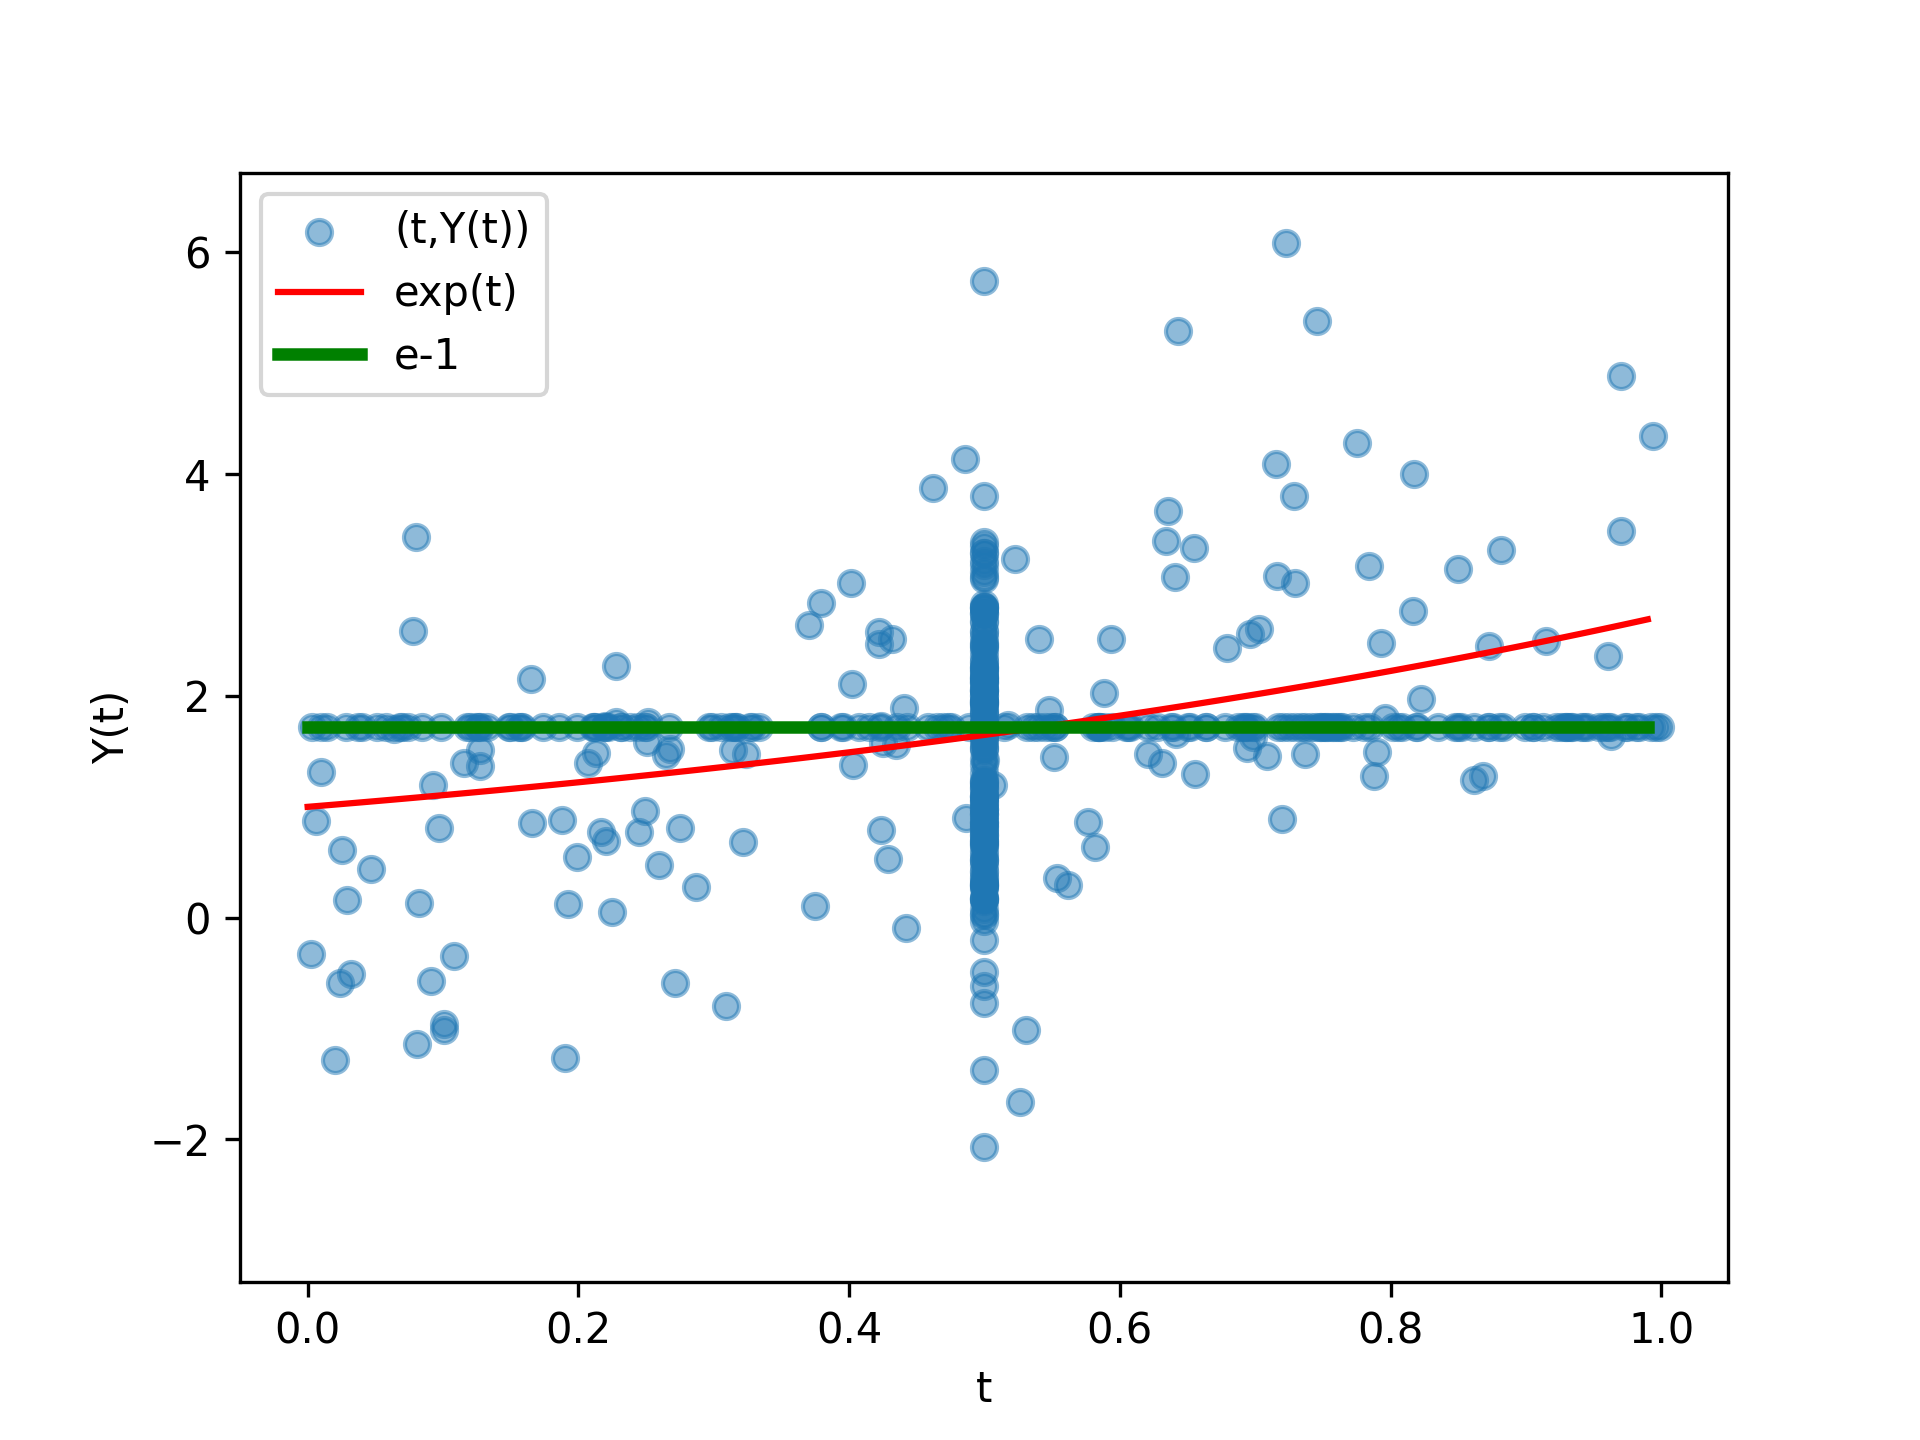
\includegraphics[width=0.8\textwidth]{plots/ydy_int.png}
    \caption{Recursive calls $(t,Y(t))$ of (\ref{RRVE ydy int}) when
      calling $Y(0.5)$ $300$ times. Points accumulate on
      the Green's line due to the Russian roulette,
      and at  $t=0.5$ because of the first recursion call.
    }
    \label{fig:ydy int}
  \end{figure}

\end{example}

(\ref{int ydy int}) is a Fredholm integral
equation of the second kind.

\begin{definition}[Fredholm equation of the second kind]
  A Fredholm equation of the second kind for $\varphi$  is of the following form:
  \begin{equation}
    \varphi(t)=f(t)+\lambda \int_a^b K(t, s) \varphi(s) ds.
  \end{equation}
  Here, $K(t, s)$ represents a kernel, and $f(t)$ is a given function.
\end{definition}

If both $K$ and $f$ satisfy certain regularity conditions, then for sufficiently
small $\lambda$, it is relatively straightforward to establish the existence
and uniqueness of solutions using a fixed-point argument.

\begin{example}[Dirichlet $y_{tt}=y$] \label{main dirichlet}
  Consider following BVP:
  \begin{equation} \label{eq:main dirichlet}
    y_{tt}=y.
  \end{equation}
  With boundary conditions $y(b_{0}),y(b_{1})$. The Green's functions corresponding to $y_{tt}$ and Dirichlet conditions are:

  \begin{align}
    P(t|x) & = \begin{cases}
                 \frac{b_{1}-t}{b_{1}-b_{0}} & \text{if } x = b_{0} \\
                 \frac{t-b_{0}}{b_{1}-b_{0}} & \text{if } x = b_{1}
               \end{cases},       \\
    G(t,s) & = \begin{cases}
                 -\frac{(b_{1}-t)(s-b_{0})}{b_{1}-b_{0}} & \text{if } s<t \\
                 -\frac{(b_{1}-s)(t-b_{0})}{b_{1}-b_{0}} & \text{if } t<s
               \end{cases}.
  \end{align}
  Directly from these Green's functions, we obtain the following integral equation and RRVE:
  \begin{align} \label{inteq:main dirichlet}
    y(t) & = P(t|b_{0}) y(b_{0}) + P(t|b_{1}) y(b_{1}) +
    \int_{b_{0}}^{b_{1}} G(t,s)y(s) ds,                  \\
    Y(t) & = P(t|b_{0}) y(b_{0}) + P(t|b_{1}) y(b_{1})
    + l B\left(\frac{1}{l} \right)(b_{1}-b_{0}) G(t,S)y(S) , \label{RRVE:main dirichlet}
  \end{align}
  with the Russian roulette rate $l \in \mathbb{R}$  and
  $S \sim \text{Uniform}(b_{0},b_{1})$. In Figure \ref{fig:plots/main_dirichlet_viz.png} and \ref{fig:mainD explosion}
  we test convergence of (\ref{RRVE:main dirichlet}).
\end{example}

\begin{figure}[h!]
  \centering
  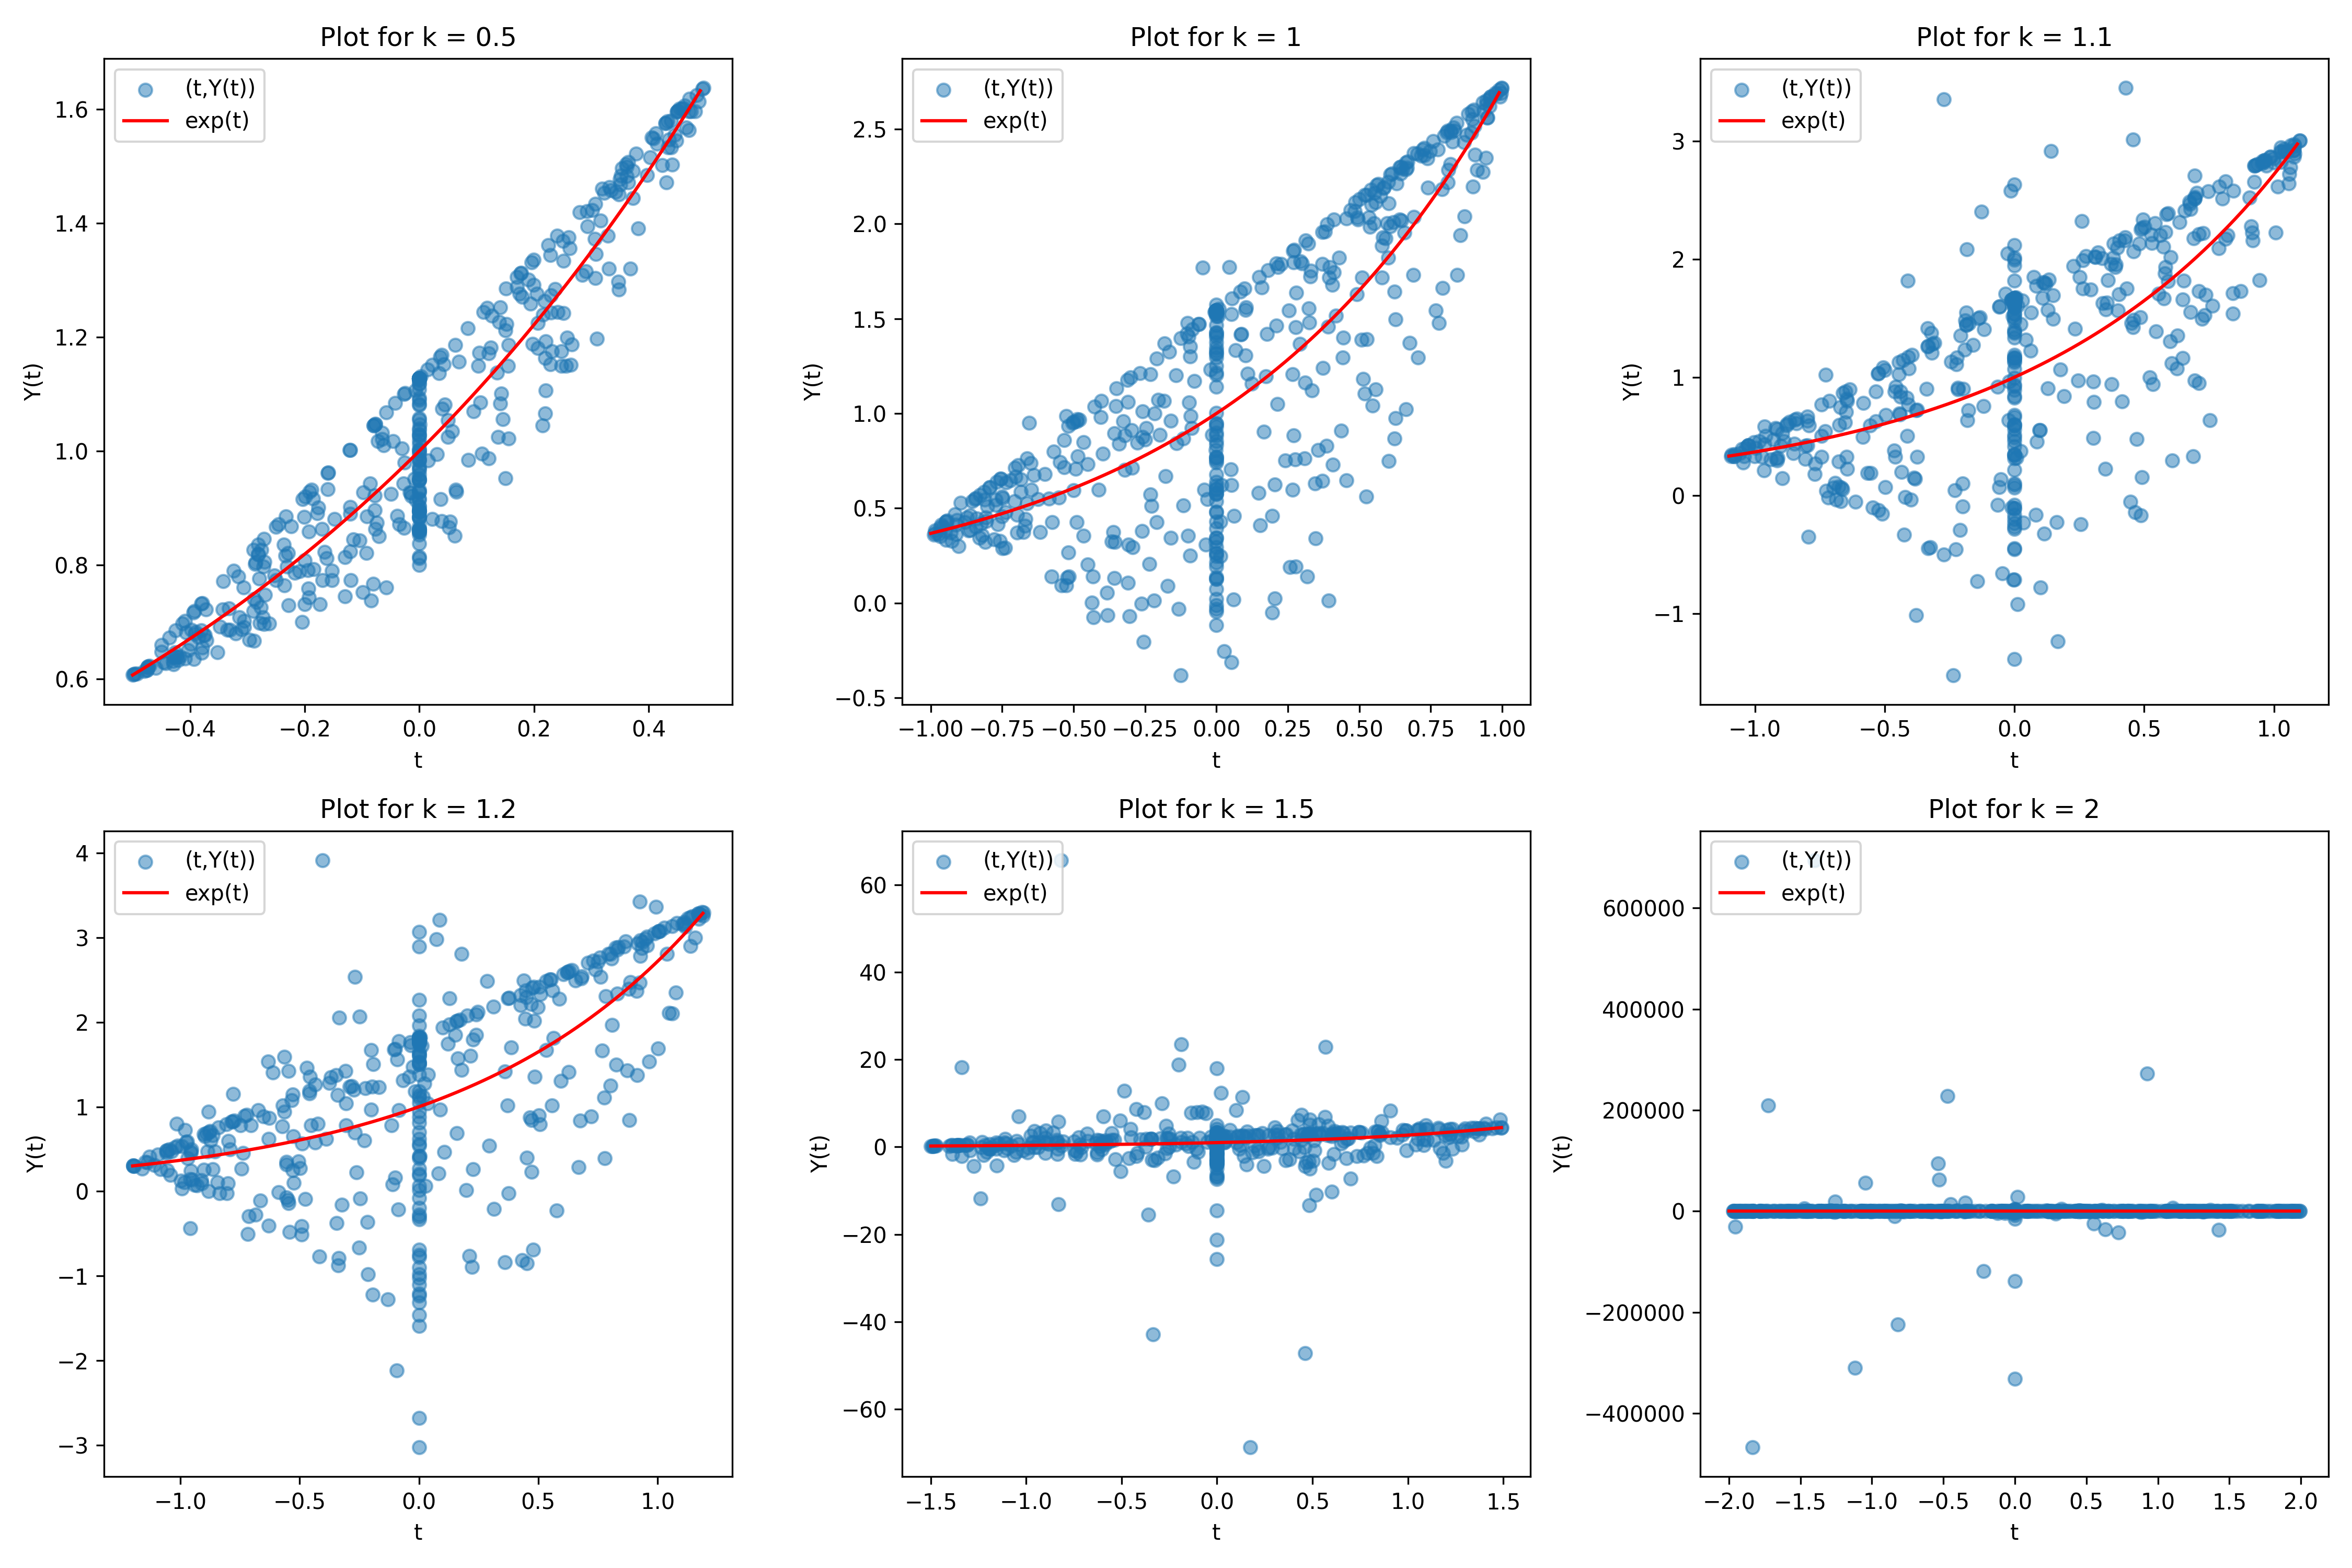
\includegraphics[width=\textwidth]{plots/main_dirichlet_viz.png}
  \caption{Recursive calls $(t,Y(t))$ of (\ref{RRVE:main dirichlet}) when
  calling $Y(0)$ $75$ times, with $l=1.2$ and boundary conditions
  $y(-k)=e^{-k}$ and $y(k)=e^{k}$.
  }
  \label{fig:plots/main_dirichlet_viz.png}
\end{figure}


\begin{figure}[h!]
  \centering
  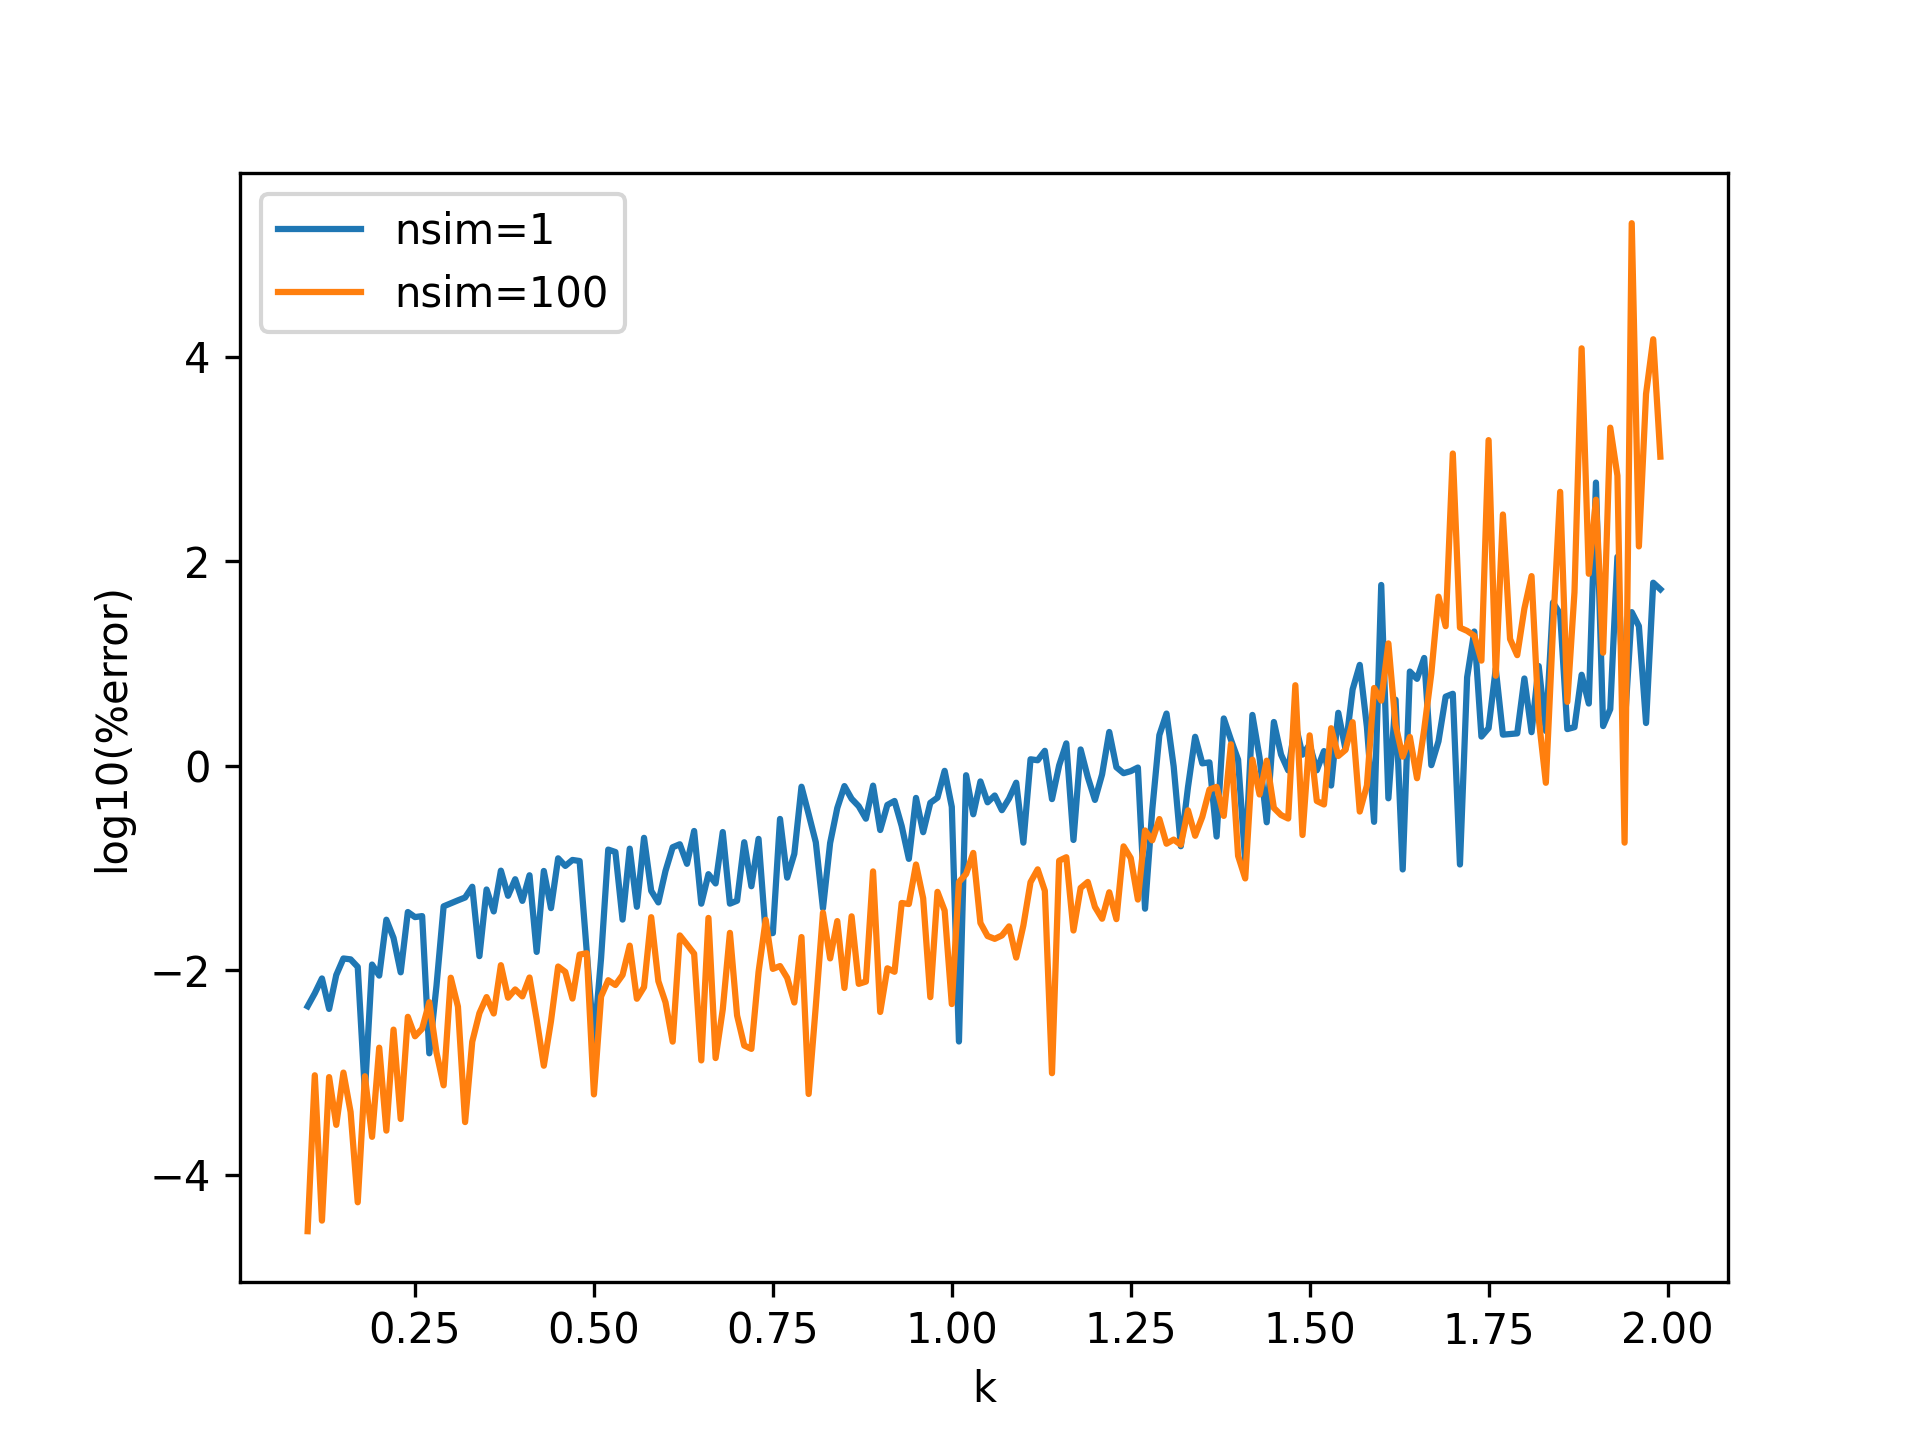
\includegraphics[width=0.8\textwidth]{plots/main_dirichlet_convergence.png}
  \caption{The logarithmic percentage error of $Y(0)$ for
  (\ref{RRVE:main dirichlet}), with $l=1.2$ and boundary conditions
  $y(-k)=e^{-k}$ and $y(k)=e^{k}$, displays an exponential
  increase until approximately $k=1.5$, beyond which additional
  simulations fail to reduce the error, indicating that the variance
  does not exist.}
  \label{fig:mainD explosion}
\end{figure}




We tested coupled splitting on Example \ref{main dirichlet}.
Coupled splitting removes the additive branching of splitting by coupling (reusing)
samples.

\begin{example}[coupled splitting on Example \ref{main dirichlet}] \label{ex:coupled splitting}
  In addition to normal splitting (see definition \ref{def:splitting}),
  we can also split the domain in (\ref{inteq:main dirichlet})
  as follows:

  % y(t) & = P(t|b_{0}) y(b_{0}) + P(t|b_{1}) y(b_{1}) +
  % \frac{1}{2} \int_{b_{0}}^{b_{1}} G(t,s)y(s) ds +
  % \frac{1}{2} \int_{b_{0}}^{b_{1}} G(t,s)y(s) ds,                                             \\

  \begin{align}\label{inteq:coupled splitting}
    y(t_1) & = P(t_1|b_{0}) y(b_{0}) + P(t_1|b_{1}) y(b_{1})                \\
           & + \int_{b_{0}}^{\frac{b_{0}+b_{1}}{2}} G(t_1,s_1)y(s_1) ds_1 +
    \int_{\frac{b_{0}+b_{1}}{2}}^{b_{1}} G(t_1,s_2)y(s_2) ds_2              \\ \label{inteq:coupled domain splitting}
    y(t_2) & = P(t_2|b_{0}) y(b_{0}) + P(t_2|b_{1}) y(b_{1})                \\
           & + \int_{b_{0}}^{\frac{b_{0}+b_{1}}{2}} G(t_2,s_1)y(s_1) ds_1
    +\int_{\frac{b_{0}+b_{1}}{2}}^{b_{1}} G(t_2,s_2)y(s_2) ds_2.
  \end{align}

  By coupling, we can eliminate the additive branching recursion
  in the RRVEs corresponding to (\ref{inteq:coupled splitting})
  and (\ref{inteq:coupled domain splitting}). In other words,
  to estimate $y(t_1)$ and $y(t_2)$ we need to estimate $y(s_1)$ and $y(s_2)$
  instead of doing it twice we reuse the same estimate.

  This results in the following RRVE:

  \begin{equation} \label{RRVE:coupled splitting}
    X(t_{1},t_{2})=
    \begin{bmatrix}
      P(t_{1}|b_{0}) & P(t_{1}|b_{1}) \\
      P(t_{2}|b_{0}) & P(t_{2}|b_{1})
    \end{bmatrix}
    \begin{bmatrix}
      y(b_{0}) \\
      y(b_{1})
    \end{bmatrix}
    +
    W
    \begin{bmatrix}
      G(t_{1},S_{1}) & G(t_{1},S_{2}) \\
      G(t_{2},S_{1}) & G(t_{2},S_{2})
    \end{bmatrix}
    X(S_{1},S_{2}),
  \end{equation}
  \juliacode{julia_code/coupled_splitting.jl}
  with $W$ some weighting matrix,
  $S_{1}$ and $S_{2}$ can be chosen
  in various ways. (\ref{RRVE:coupled splitting}) is unbiased in the following way:
  $X(t_{1},t_{2}) \cong [y(t_{1}) \quad y(t_{2})]^{T}$.

\end{example}

\begin{figure}[h!]
  \centering
  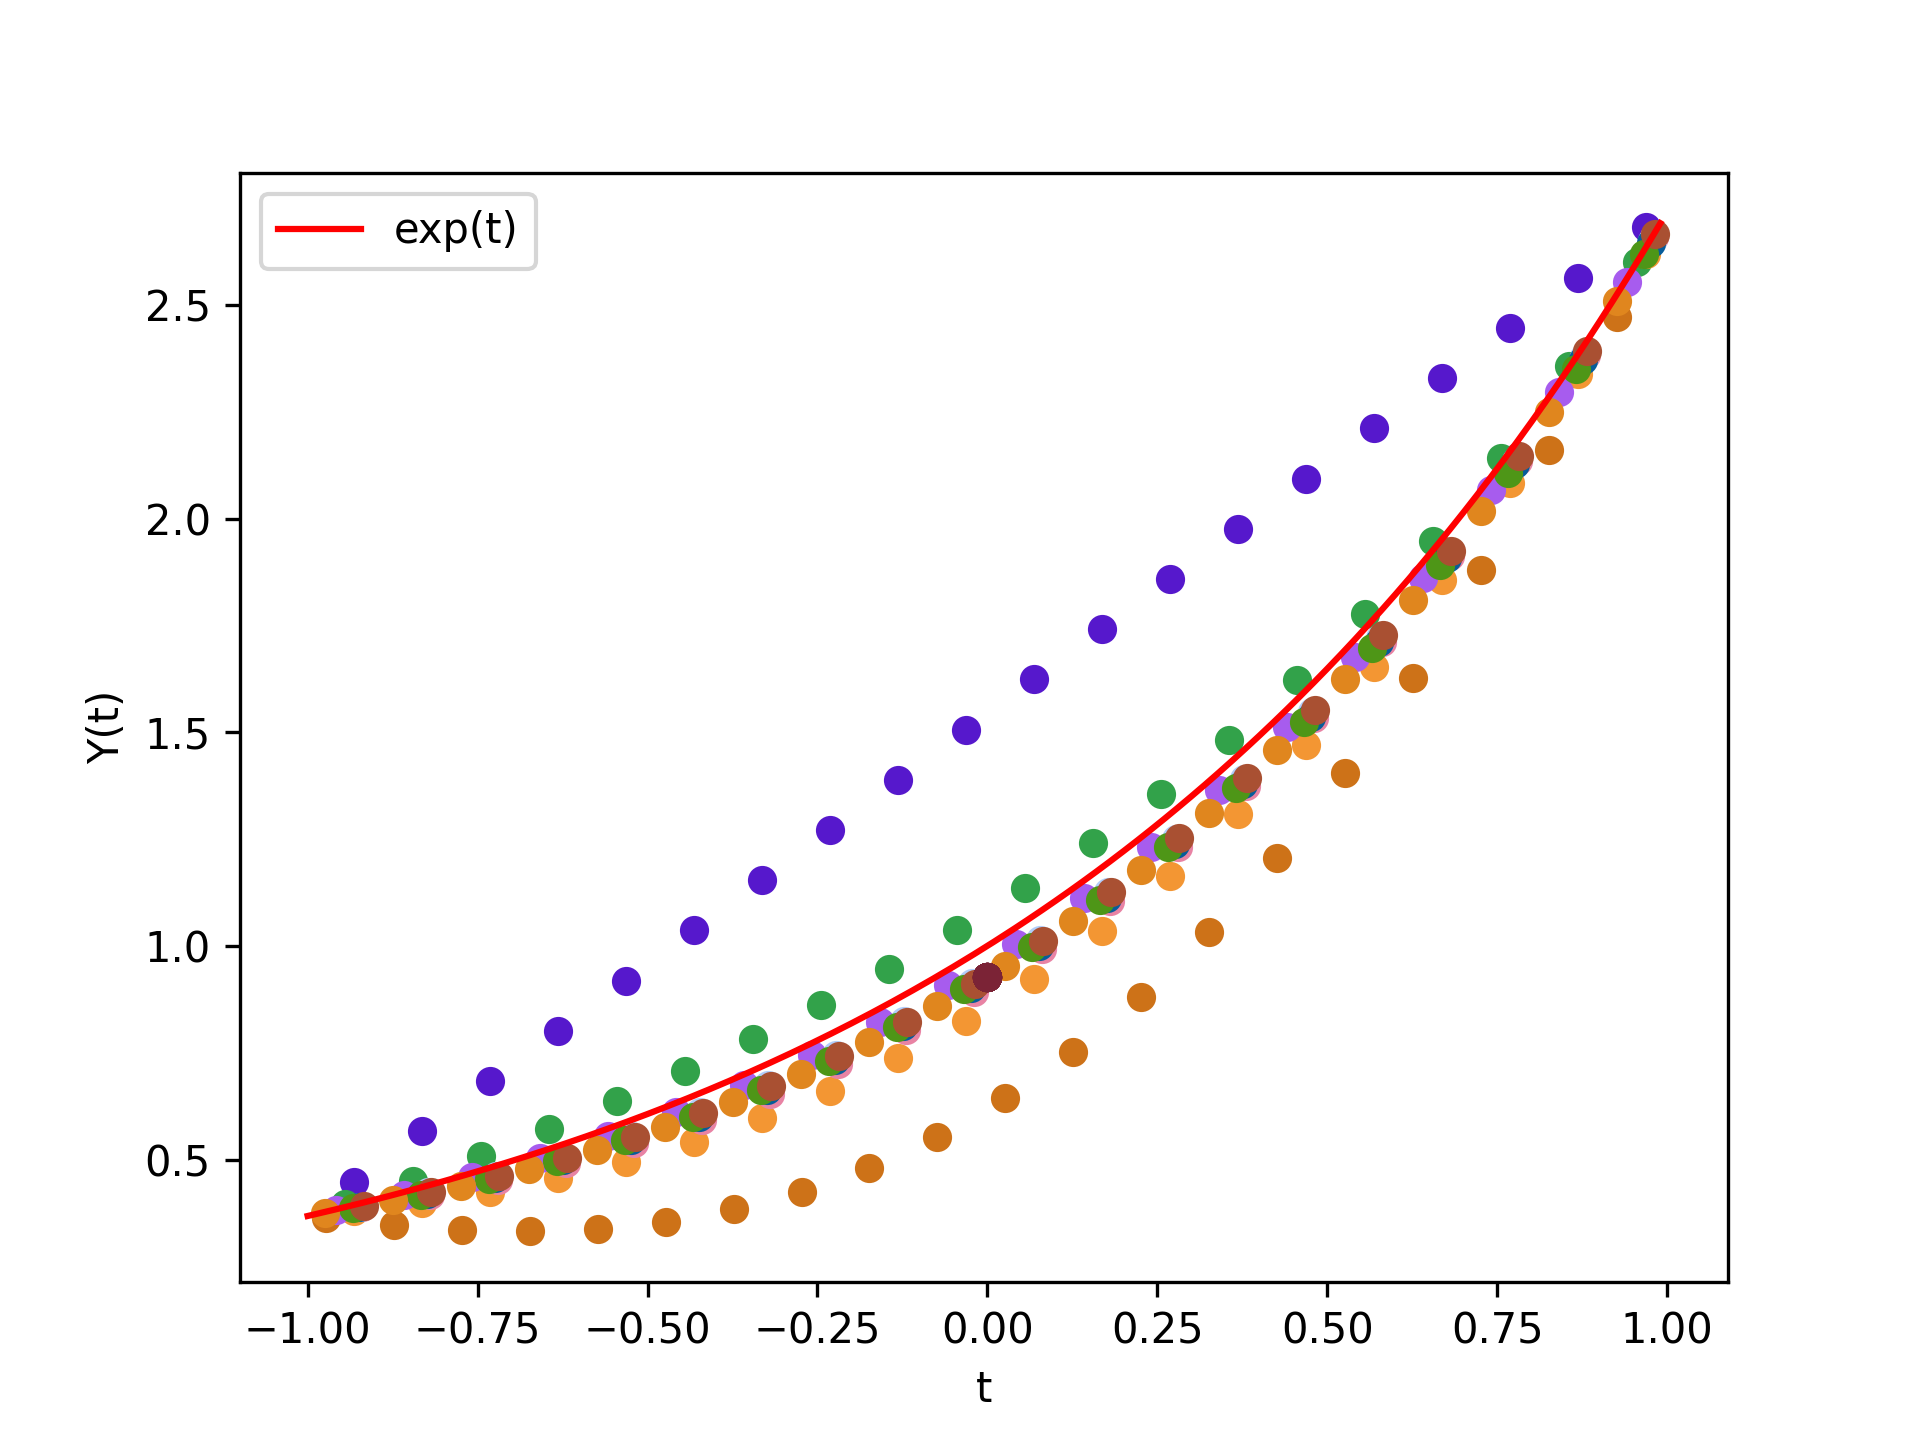
\includegraphics[width=0.8\textwidth]{plots/coupled_split.png}
  \caption{Recursive calls of (\ref{RRVE:coupled splitting}) when
  calling $X(0)$ once. We chose $X$ to have $20$ points and
  colored each call. The $S_{j}$ are coupled such that
  they are equally spaced.
  The initial conditions for this call are $y(-1)=e^{-1}$ and $y(1)=e^{1}$,
  with Russian roulette rate $l=1.2$. }
  \label{fig:coupled splitting}
\end{figure}

% \begin{pythonn}[implementation of (\ref{RRVE:coupled splitting})] \label{py:coupled splitting}
%     We implemented (\ref{RRVE:coupled splitting}) with recursion. In this case,
%     a forward implementation is more efficient. \\
%     \pythoncode{python code/coupled_splitting.py}

% \end{pythonn}

\begin{related}[coupled splitting]
  Coupled splitting is partly inspired by the approach
  of \cite{sabelfeld_sparsified_2009}, which reduces
  variance by using larger submatrices in unbiased sparsification
  of matrices.
  Reusing samples for WoS is discussed in both
  \cite{miller_boundary_2023} and \cite{bakbouk_mean_2023}.
\end{related}

Figure \ref{fig:coupled splitting}
resembles fixed-point iterations, leading us to hypothesize
that the convergence
speed is very similar to fix-points methods until the accuracy
of the stochastic approximation of the operator is reached
(the approximate operator bottleneck). The approximation of the operator
can be improved by increasing the coupled splitting amount when
approaching the bottleneck. Alternatively when reaching
the bottleneck it is possible to rely on splitting to converge.

\begin{related}[convergence coupled splitting]
  See \cite{gupta_convergence_2021} for a discussion on the convergence
  of recursive stochastic algorithms.
\end{related}


\begin{related}[IBC integral equations]
  Optimal IBC is known for integral equations see \cite{heinrich_monte_1998}
  for the solution at $1$ point and the global solution.
\end{related}

\subsection{Initial Value Problems}
Classic IVP solvers rely on shrinking the time steps for
convergence. In this subsection, we introduce
Recursion in Recursion MC (RRMC) for IVPs which tries to emulate
this behavior.


\begin{example}[RRMC $y_t=y$] \label{ex:RRMC IVP}
  We demonstrate RRMC for IVPs with

  \begin{equation}
    y_t = y, \quad y(0) = 1.
  \end{equation}

  Imagine we have a time-stepping scheme $(t_{n}), \forall n: t_{n-1} < t_{n}$
  then the following integral equations hold:

  \begin{equation}
    y(t)= y(t_{n}) + \int_{t_{n}}^{t}y(s)ds , \quad t>t_{n}.
  \end{equation}

  Turn these in the following class of RRVEs:

  \begin{equation}
    y(t) \cong Y_{j}(t) = y(t_{j}) + (t-t_{j})Y_{j}((t-t_{j})U+t_{j}), \quad t>t_{j}.
  \end{equation}

  A problem with these RRVEs is that we do not know $y(t_{j})$.
  Instead, we can replace it with an unbiased estimate $y_{j}$
  which we keep fixed in the inner recursion:
  \begin{align}
    \label{eq:RRMC IVP inner}
    y(t) \cong Y_{j}(t)  & = y_{j} + (t-t_{j})Y_{j}((t-t_{j})U+t_{j}), \quad t>t_{j} \\
    y(t_{j}) \cong y_{j} & = \begin{cases}
                               Y_{j-1}(t_{j}) & \text{ if } j \neq 0 \\
                               y(t_{0})       & \text{ if } j = 0
                             \end{cases}.
    \label{eq:RRMC IVP outer}
  \end{align}
  \juliacode{julia_code/RRMC_IVP.jl}
  We refer to (\ref{eq:RRMC IVP inner}) as the inner recursion and
  (\ref{eq:RRMC IVP outer}) as the outer recursion of the recursion in
  recursion.
  The measured RMSE for estimating $y(t)$ is of the order
  $O\left(h^{1.5} \right)$, where $h$ represents
  the step size. For the implementation we used a scaled version
  of the time process from Example \ref{ex: russian roulette}
  for the inner recursion, such that the average number of total inner recursion calls
  is $e n$, where $n$ represents the total number of outer recursion calls.
\end{example}

% \begin{pythonn}[implementation of Example \ref{ex:RRMC IVP}] \label{py:RRMC IVP}
%     \pythoncode{python code/RRMC_IVP.py}

%     \begin{figure}[h!]
%         \centering
%         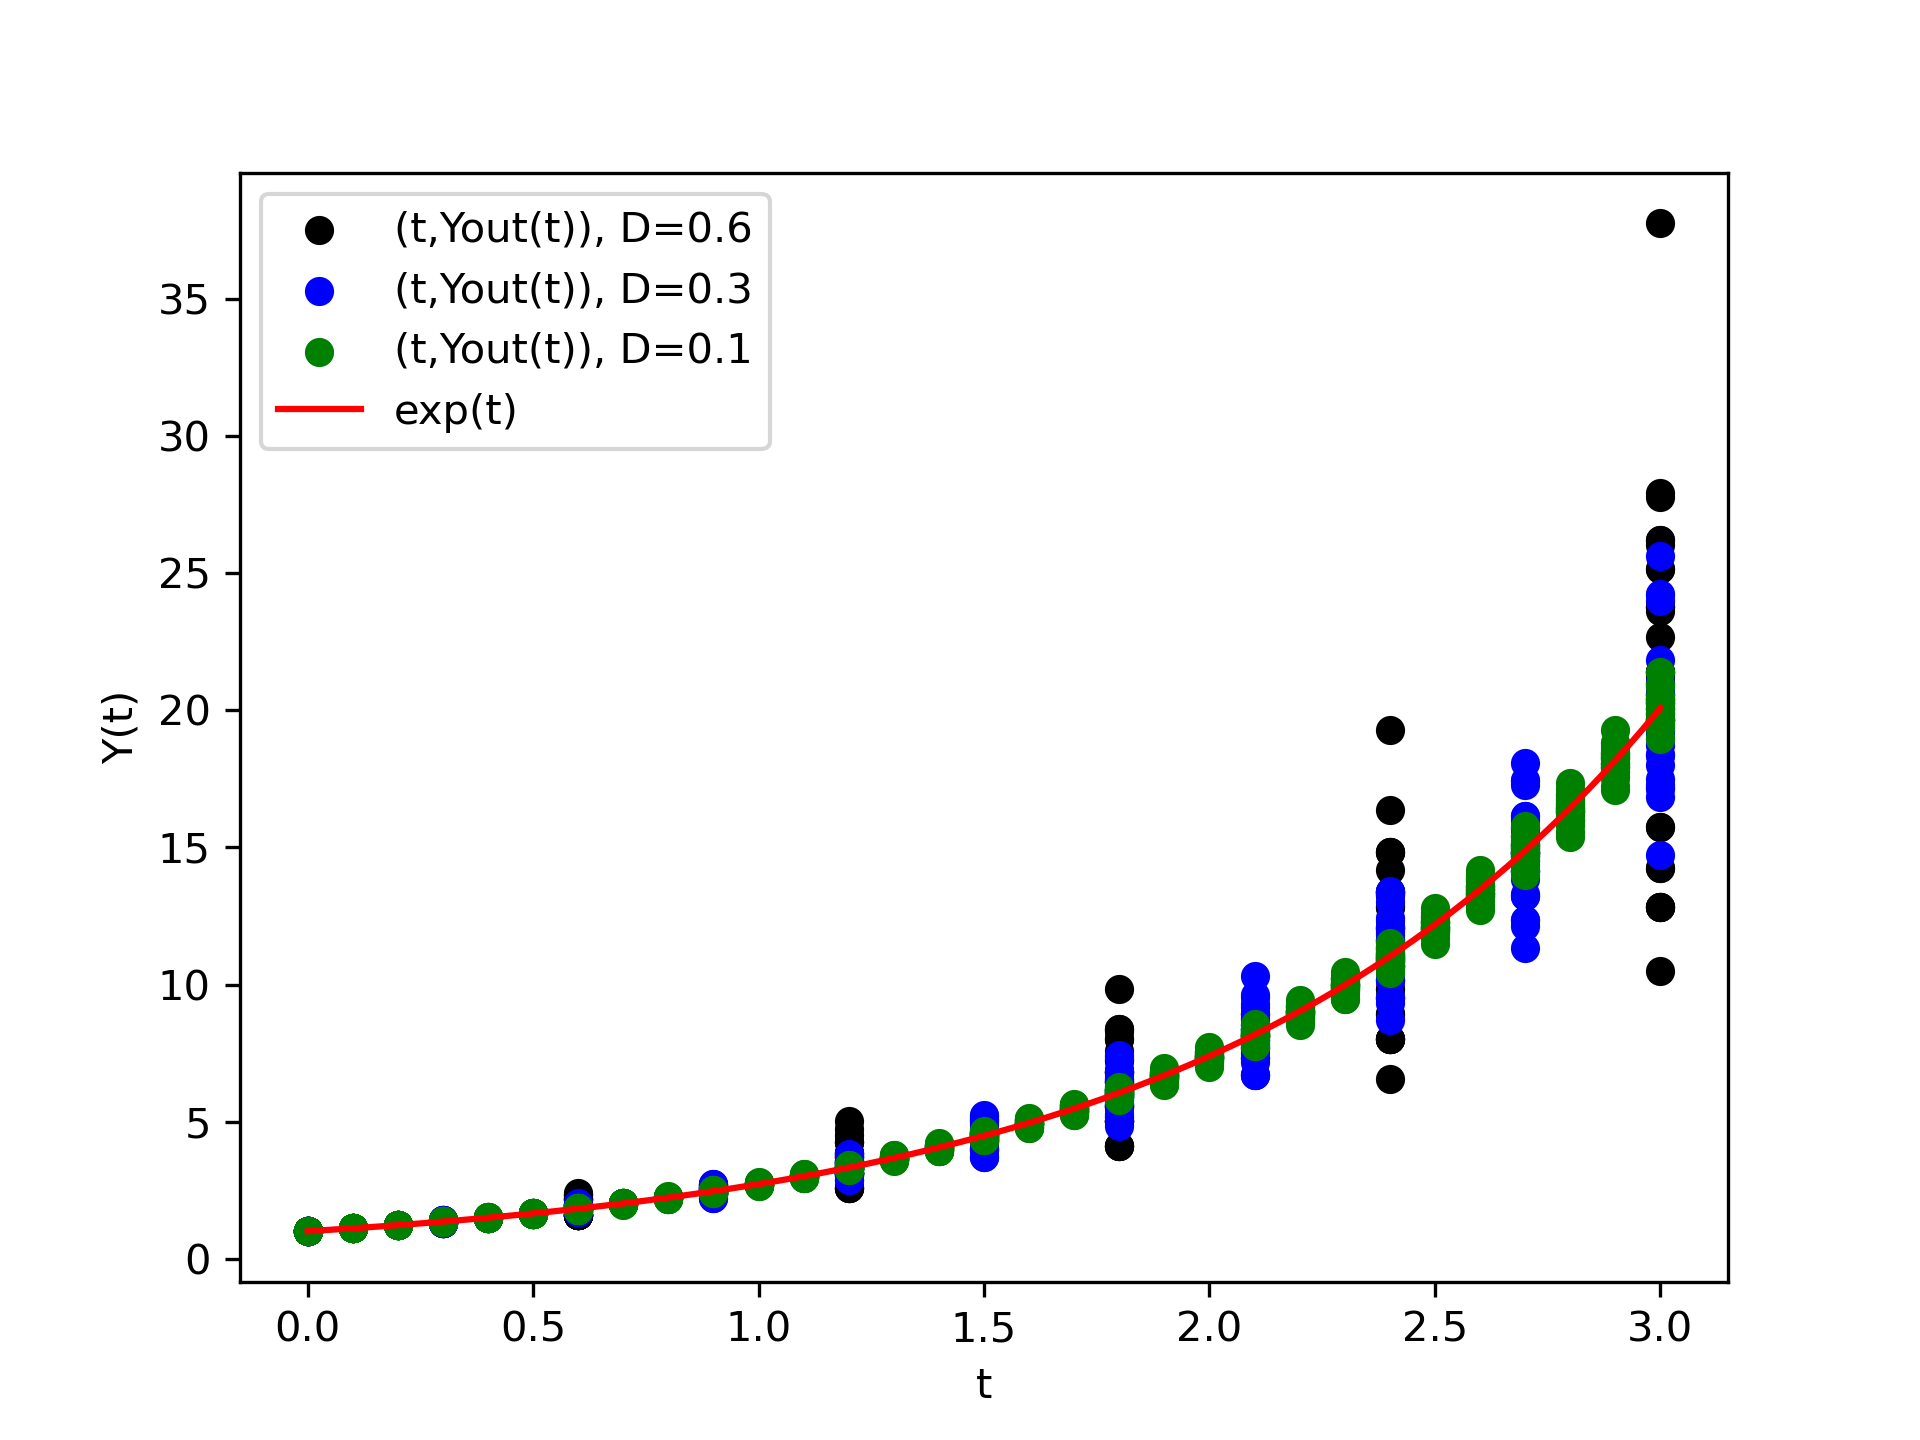
\includegraphics[width=0.8\textwidth]{plots/RRMC IVP.png}
%         \caption{Recursive calls of (\ref{eq:RRMC IVP outer})
%             when calling $Y_{\text{out}}(3,h)$ $30$ times for different $h$.  }
%         \label{fig:RRMC IVP}
%     \end{figure}
% \end{pythonn}


\begin{conjecture}[local RMSE RMC]
  Consider a general linear IVP:
  \begin{equation}
    y_{t}(t)= A(t)y(t)+g(t), y(t_{0}),
  \end{equation}
  with $A$ a matrix and $g$ a vector function, each
  once differentiable with the corresponding RRVE:
  \begin{equation}
    y(t) \cong Y(t) = y(t_{0}) + h B \left( \frac{t-t_{0}}{h}\right)
    A(S) Y(S) + g(S),
  \end{equation}
  where $S \sim \text{Uniform}(t_{0},t)$. Then, the following relation holds:
  \begin{equation}
    E[||y(t_{1})-Y(t_{1})||^{2}] = O(h^{2}),
  \end{equation}
  with $t_{1} = t_{0} + h$.
\end{conjecture}


To achieve a higher order of convergence RRMC can be combined with control variates.
\begin{example}[CV RRMC $y_t=y$]\label{ex:CV RRMC IVP}
  Let us control variate Example \ref{ex:RRMC IVP}.

  \begin{equation}
    y(t)= y(t_{n}) + \int_{t_{n}}^{t}y(s)ds , \quad t>t_{n}.
  \end{equation}

  We build a control variate with a lower-order approximation
  of the integrand:

  \begin{align}
    y(s) & = y(t_{n}) + (s-t_{n})y_t(t_{n}) + O((s-t_{n})^{2})      \\
         & \approx y(t_{n}) + (s-t_{n})f(y(t_{n}),t_{n})            \\
         & \approx y(t_{n}) +
    (s-t_{n})\left(\frac{y(t_{n})-y(t_{n-1})}{t_{n}-t_{n-1}}\right) \\
         & \approx y(t_{n})(1+s-t_{n}). \label{eq:CVCV RRMC}
  \end{align}

  Using (\ref{eq:CVCV RRMC}) as a control variate for the integral:

  \begin{align}
    y(t) & = y(t_{n}) + \int_{t_{n}}^{t}y(s)ds                                          \\
         & = y(t_{n}) + \int_{t_{n}}^{t}y(s)-y(t_{n})(1+s-t_{n}) +y(t_{n})(1+s-t_{n})ds \\
         & = y(t_{n})\left(1 + (1-t_{n})(t-t_{n})+\frac{t^{2}-t_{n}^{2}}{2}\right)
    + \int_{t_{n}}^{t}y(s)-y(t_{n})(1+s-t_{n})ds. \label{eq: int CV RRMC}
  \end{align}

  Figure \ref{fig:CV RRMC IVP} displays the error
  of realizations of an RRVE constructed from (\ref{eq: int CV RRMC})
  for various step sizes.

  \begin{figure}[h!]
    \centering
    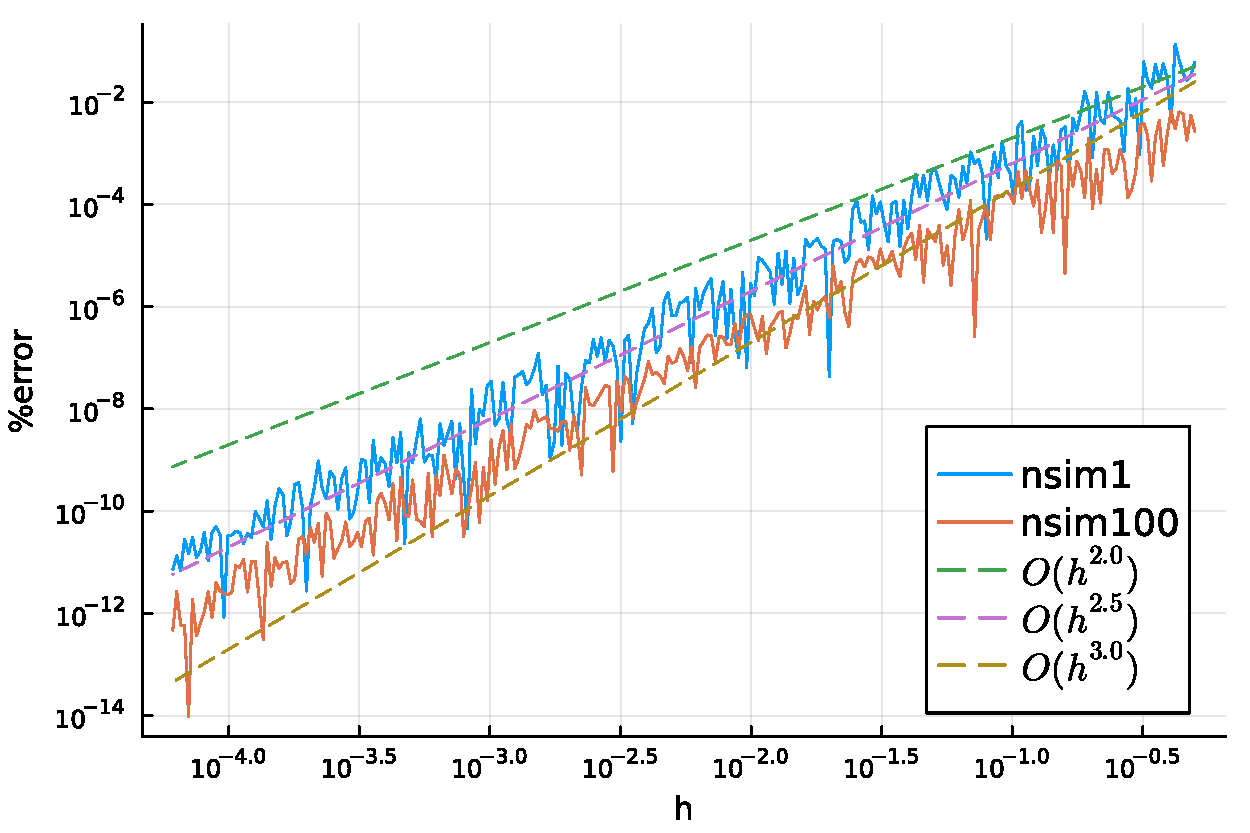
\includegraphics[width=0.8\textwidth]{julia_plots/CV_RRMC_IVP.pdf}
    \caption{Log-log plot of the error for Example
      \ref{ex:CV RRMC IVP} at $Y(10)$.}
    \label{fig:CV RRMC IVP}
  \end{figure}
\end{example}

\begin{related}[CV RRMC]
  \cite{daun_randomized_2011} similarly uses control variates to achieve
  a higher order of convergence.
\end{related}

Similar to explicit solvers, RRMC performs poorly on stiff problems.
We attempted to make RRMC more like implicit solvers but this proved difficult.
Instead, we believe that an approach more like exponential integrators
is more viable.
% We experimented with Diagonal RRMC in this direction with
% little success.

% \begin{definition}[Diagonal RRMC] \label{def:DRRMC}
%     Consider a general linear ODE IVP problem:
%     \begin{equation}
%         x' = Ax+g, \quad x(0)= x_{0}.
%     \end{equation}
%     In some cases, repeatedly multiplying by matrix $A$ can lead to instability.
%     Diagonal RRMC attempts to address this issue by adding a positive diagonal matrix $D$
%     to matrix $A$ .

%     \begin{equation}
%         x' + Dx = (A+D)x+g.
%     \end{equation}

%     The following integral equation can be derived by using integrating factor:

%     \begin{equation}\label{eq:int eq DRRMC}
%         x(t)= e^{D(t_{n}-t)}x(t_{n}) + \int_{t_{n}}^{t} e^{D(s-t)}(A(s)+D)x(s)ds+\int_{t_{n}}^{t} e^{D(s-t)}g(s)ds.
%     \end{equation}

%     The recursive integral has the following trivial control variate:

%     \begin{equation}\label{eq: CV DRRMC}
%         \int_{t_{n}}^{t}  e^{D(s-t)}(A(t_{n})+D)x(t_{n})ds = D^{-1}(I-e^{D(t_{n}-t)})(A(t_{n})+D)x(t_{n}).
%     \end{equation}

%     Note that $D$ may be chosen differently for every outer recursion.
% \end{definition}

% \begin{example}[DRRMC] \label{ex:DRRMC}
%     Consider:
%     \begin{equation}
%         x'= Ax, x(0)=
%         \begin{bmatrix}
%             1 \\
%             0
%         \end{bmatrix}.
%     \end{equation}

%     With

%     \begin{equation}
%         A = \begin{bmatrix}
%             0     & 1     \\
%             -1000 & -1001
%         \end{bmatrix}.
%     \end{equation}

%     This has the following solution:

%     \begin{equation}
%         x(t) = \frac{1}{999}
%         \begin{bmatrix}
%             -  e^{-1000t}+ 1000 e^{-t} \\
%             1000 e^{-1000t}- 1000e^{-t}
%         \end{bmatrix}.
%     \end{equation}

%     We choose $D$ fixed across outer recursions:

%     \begin{equation}
%         D = \begin{bmatrix}
%             1 & 0    \\
%             0 & 1000
%         \end{bmatrix}.
%     \end{equation}

%     We make a convergence plot for this example with
%     (\ref{eq:int eq DRRMC}) with control variate
%     (\ref{eq: CV DRRMC}) implemented with recursion in recursion
%     on Figure \ref{fig:DRRMC}.

%     \begin{figure}[h!]
%         \centering
%         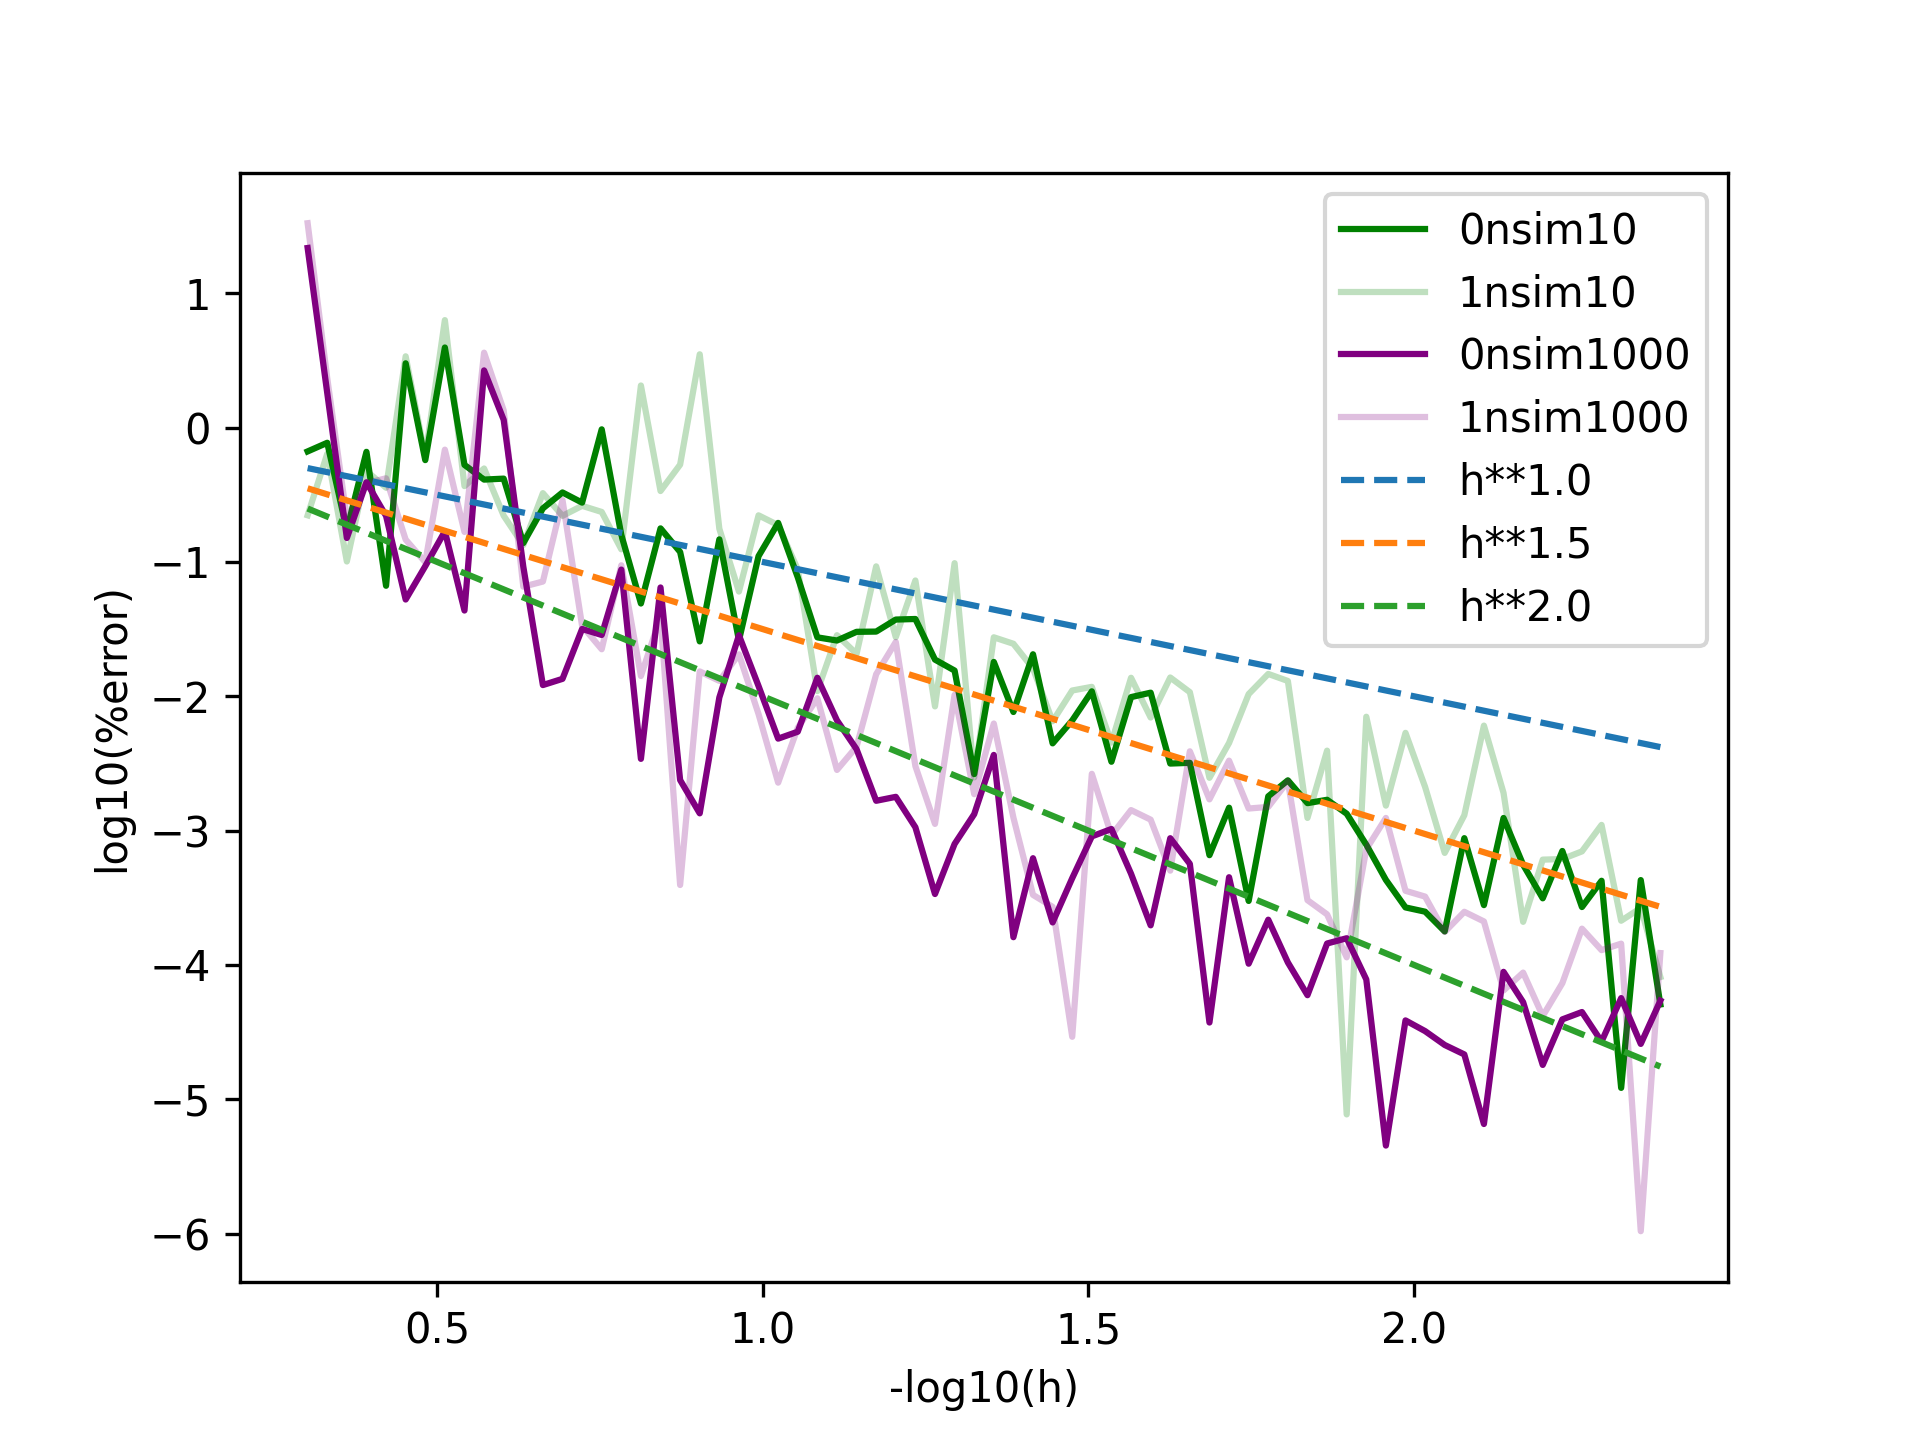
\includegraphics[width=0.8\textwidth]{plots/DRRMC.png}
%         \caption{Log-log plot of the error of Example \ref{ex:DRRMC}.
%             We plotted the second component of the error transparent.
%         }
%         \label{fig:DRRMC}
%     \end{figure}

% \end{example}

% \begin{related}[DRRMC]
%     DRRMC is inspired by the $\bar{\sigma}$ parameter in \cite{sawhney_grid-free_2022}.
%     However, instead of relying on importance sampling, we employ control
%     variates to address the nonlinearity introduced by the exponential
%     function.
% \end{related}

% \section{Brownian Motion}


% \begin{definition}[Brownian motion]
%     Define Brownian motion $W_{t}$ as the limit/logical generalization
%     when $n \rightarrow \infty$ of the following discrete process is defined as:
%     \begin{equation}
%         \begin{cases}
%             X_{t}^{n} = X_{t-\frac{1}{n}}^{n} + Z_{n} \\
%             X^{n}_{0}=0
%         \end{cases}.
%     \end{equation}
%     With $Z_{n}\sim N(0,\frac{1}{n})$ i.i.d . From this definition it is easily seen that
%     $W_{t} \sim N(0,t)$.
% \end{definition}


% \begin{lemma}[self-affinity Brownian motion] \label{lem:self affine}
%   Brownian motion is a self-affine random process, which implies
%   that any subpath can be translated and scaled in such a way
%   that its distribution matches that of the entire path.

% \end{lemma}


\section{Heat Equation}

In this section we discuss how to solve ODEs derived from the semi-discretized heat equation
with Dirichlet boundary conditions in $1$ point and acceleration with recursive first-passage sampling
combined with presampled path stitching.

% \begin{definition}[$1$D heat equation Dirichlet general domain] \label{def:heat equation}
%     We define the $1$D heat equation for $u$ on connected domain $\Omega$
%     with  Dirichlet boundary conditions the following way:
%     \begin{equation}
%         \frac{\partial u}{\partial t} = \frac{\partial^{2} u}{\partial x ^{2}}.
%     \end{equation}
%     Given $u(x,t)=\psi(x,t) ,\forall (x,t) \in \partial \Omega: t<\sup \{
%         t| (x,t) \in \Omega\}$ .
% \end{definition}

% % maybe should improve this 
% Figure \ref{fig:Euler first passage para} shows how the Dirichlet condition
% is defined for parabola but reverse in time.

\begin{definition}[1D heat equation Dirichlet] \label{def:heat equation square}
  We define the 1D heat equation for $u(x,t)$ with $ (x,t) \in \Omega = [0,1]^2$
  with Dirichlet boundary conditions the following way:
  \begin{align}
    \frac{\partial u}{\partial t} & = \frac{\partial^{2} u}{\partial x^{2}}  \Leftrightarrow   \\
    u_t(x,t)                      & = u_{xx}(x,t), \quad \forall (x,t) \in \Omega = [0,1]^2  .
  \end{align}
  Given $\left\{u(x,0),u(1,t),u(0,t) | \forall x,t \in [0,1]  \right\} $.
\end{definition}

\begin{definition}[semi-discretization 1D heat equation Dirichlet] \label{def:discrete heat equation square}
  We define the semi-discretization 1D heat equation for $\tilde{u}$ as space discretized heat equation
  using the central difference scheme:

  \begin{equation}
    \tilde{u}_t(j \Delta x,t)  = \frac{\tilde{u}((j+1) \Delta x, t)-2\tilde{u}(j \Delta x, t)+\tilde{u}((j-1) \Delta x, t)}{\Delta x^{2}}
  \end{equation}
  $\forall (j,t) \in \{0, 1, \ldots, N\} \times [0,1]$. \\
  Given $\left\{\tilde{u}(j \Delta x,0),\tilde{u}(1,t),\tilde{u}(0,t) | \forall j \in \{0, 1, \ldots, N\}, \forall t \in  [0,1]  \right\} $.
\end{definition}


% maybe we need to find a reference for this
It is well-known that the solution to the semi-discretization 1D heat equation converges to the solution of the 1D heat equation with
corresponding boundary conditions as $\Delta x \rightarrow 0$. \\
We want a point estimator for the solution to the semi-discretization 1D heat equation. We obtain this by
using (\ref{eq:poisson main}) with $\sigma = \frac{2}{\Delta x^{2}}$ and at the interior point $j$ this is:

% \begin{align}
%     \tilde{u}_t(j \Delta x,t)                                                 & = \frac{\tilde{u}((j+1) \Delta x, t)-2\tilde{u}(j \Delta x, t)+\tilde{u}((j-1) \Delta x, t)}{\Delta x^{2}} \\
%     \tilde{u}_t(j \Delta x,t) + \frac{2}{\Delta x^{2}}\tilde{u}(j \Delta x,t) & = \frac{\tilde{u}((j+1) \Delta x, t)+\tilde{u}((j-1) \Delta x, t)}{\Delta x^{2}}
% \end{align}

% Explantation of this standard ODE step.

% \begin{align}
%     \tilde{u}(j \Delta x,t) = e^{-\frac{2}{\Delta x^{2}} t} \left[\tilde{u}(j \Delta x,0)
%     + \frac{1}{\Delta x^{2}} \int_{0}^{t} e^{\frac{2}{\Delta x^{2}} s}
%     (\tilde{u}((j+1) \Delta x,s)+\tilde{u}((j-1) \Delta x,s))ds  \right].
% \end{align}

% Instead of directly uniformly sampling this integral we first do following substitution
% $\tau = e^{\frac{2}{\Delta x^{2}}(s-t)}, d\tau =\frac{2}{\Delta x^{2}}  e^{\frac{2}{\Delta x^{2}}(s-t)}ds $
% which reduces variance. Note that it is equivalent to importance sampling
% the exponential term.

% \begin{align}
%     \tilde{u}(j \Delta x,t) & = e^{-\frac{2}{\Delta x^{2}} t} \tilde{u}(j \Delta x,0)
%     + \int_{e^{-\frac{2t}{\Delta x^{2}}}}^{1} \frac{\tilde{u}((j+1) \Delta x,s)+\tilde{u}((j-1) \Delta x,s)}{2}d\tau \nonumber \\
%                             & = \int_{0}^{e^{-\frac{2t}{\Delta x^{2}}}}  \tilde{u}(j \Delta x,0) d\tau+
%     \int_{e^{-\frac{2t}{\Delta x^{2}}}}^{1} \frac{\tilde{u}((j+1) \Delta x,s)+\tilde{u}((j-1) \Delta x,s)}{2}d\tau. \label{eq:int semi heat}
% \end{align}

\begin{equation}
  \tilde{u}(j \Delta x,t) = \int_{0}^{e^{-\frac{2t}{\Delta x^{2}}}}  \tilde{u}(j \Delta x,0) d\tau+
  \int_{e^{-\frac{2t}{\Delta x^{2}}}}^{1} \frac{\tilde{u}((j+1) \Delta x,s)+\tilde{u}((j-1) \Delta x,s)}{2}d\tau. \label{eq:int semi heat}
\end{equation}



\begin{julia}[implementation of estimator of (\ref{eq:int semi heat})]\label{jl:point estimator heat}

  (\ref{eq:int semi heat}) can be turned into a estimator $Y(j \Delta x,t,\Delta x ) \cong  \tilde{u}(j \Delta x,t)$
  by sampling $\tau \sim U$,
  sampling one of the $\tilde{u}$ of the second integral to avoid branching recursion and
  recursing when $\tilde{u}$ is unknown.

  \juliacode{julia_code/point_estimator_heat_tail.jl}

  $Y(j \Delta x,t,\Delta x )$ is just the boundary condition
  for the first passage point from the time space domain for a Poisson time process and a random walk in space.
  In this implementation as  $\Delta x \rightarrow 0$  the cost of calculating the first passage time grows
  $\approx O(\Delta x ^{-2})$ and the process converges to Brownian motion. Note that the estimator needs
  only $1$ function call from the boundary conditions.
\end{julia}

\begin{example}[\ref{def:discrete heat equation square} + source + coefficients] \label{ex:semi heat source}

  Example \ref{def:discrete heat equation square}
  can be extended with a source term and $0$-order coefficients:

  \begin{equation}
    u_{t} = u_{xx} + a(x,t)u + f(x,t)
    .
  \end{equation}

  Again by using (\ref{eq:poisson main}) with $\sigma = \frac{2}{\Delta x^{2}} +a_{0}$
  looking at an interior point we obtain:

  \begin{equation}
    u =
    \int_{0}^{e^{-t \sigma }} u_{0} d\tau  + \int_{e^{-t \sigma }}^{1}
    \sigma^{-1}
    \left(
    \frac{u_{+} + u_{-}}{\Delta x^{2}} +(a(x,s)+ a_{0}) u+ f
    \right)
    d\tau
    .
  \end{equation}
  To remove branching recursion we sample one of the $u$'s, we base the sampling
  probability based on the magnitude of coefficients, let $a_m$ be approximately the magnitude of
  $(a(x,s)+ a_{0})$. We chose to sample the $(a(x,s)+ a_{0})u$ term and $f$
  with probability $p_{\text{source}} = \frac{a_m}{a_m + \frac{2}{\Delta x^{2}}}$.
  As $\Delta x \rightarrow 0$ the $\frac{u_{+} + u_{-}}{\Delta x^{2}}$ term is
  the main contribution to the second integral therefore
  being sampled almost always.
  In total for $1$ fully recursed sample,
  the $f(x,s)$ and the $(a(x,s)+ a_{0})u$ term only
  is sampled a few times and this does not scale with $\Delta x$. We
  sampled $f$ together with $(a(x,s)+ a_{0})u$ for simplicity.
\end{example}

\begin{julia}[implementation of estimator of Example \ref{ex:semi heat source}]\label{jl:point estimator heat source}
  Because of the high chance of sampling the $\frac{u_{+} + u_{-}}{\Delta x^{2}}$ it is efficient
  to sample the interarrival until not sampling it which is geometrically distributed.

  \juliacode{julia_code/pest_heat_varcoef.jl}
\end{julia}

Computing the estimator requires knowing more then the first passage point
unlike Example \ref{def:discrete heat equation square} but this is limited
to a few points of the time space process and this amount does not scale with $\Delta x$.


\begin{technique}[presampling the process of \ref{jl:point estimator heat source}] \label{tech:presampling heat}
  As $\Delta x \rightarrow 0$ the bottleneck is sampling the process that moves through space and time.
  This process is independent of the boundary conditions, $a(x,t)$ and $f(x,t)$. So it is possible to
  precompute samples of the process and reuse them for different boundary conditions, $a(x,t)$ and $f(x,t)$.
  Reusing paths makes the solutions correlated. To compute the estimator we need to know where we sampled the
  source term to update $sol$ and $w$, how many steps we took in between to update $w$ for the
  multiplications in not source points (line 13 of \ref{jl:point estimator heat source})
  and where termination happens.

  \juliacode{julia_code/genpath_pest_heat_varcoef.jl}

  Paths for smaller $\tilde{a}_{m}$'s can be obtained by thinning the Bernoulli process,
  by rejecting source points with probability $\frac{\tilde{a}_{m}}{a_{m}}$. As $\Delta x \rightarrow 0$
  $genPath$ converges, the dependence on $a_{0}$ also disappears. For the heat equation
  $genPath$ presampled paths only depend on geometry and the starting point.

  \begin{figure}[h!]
    \centering
    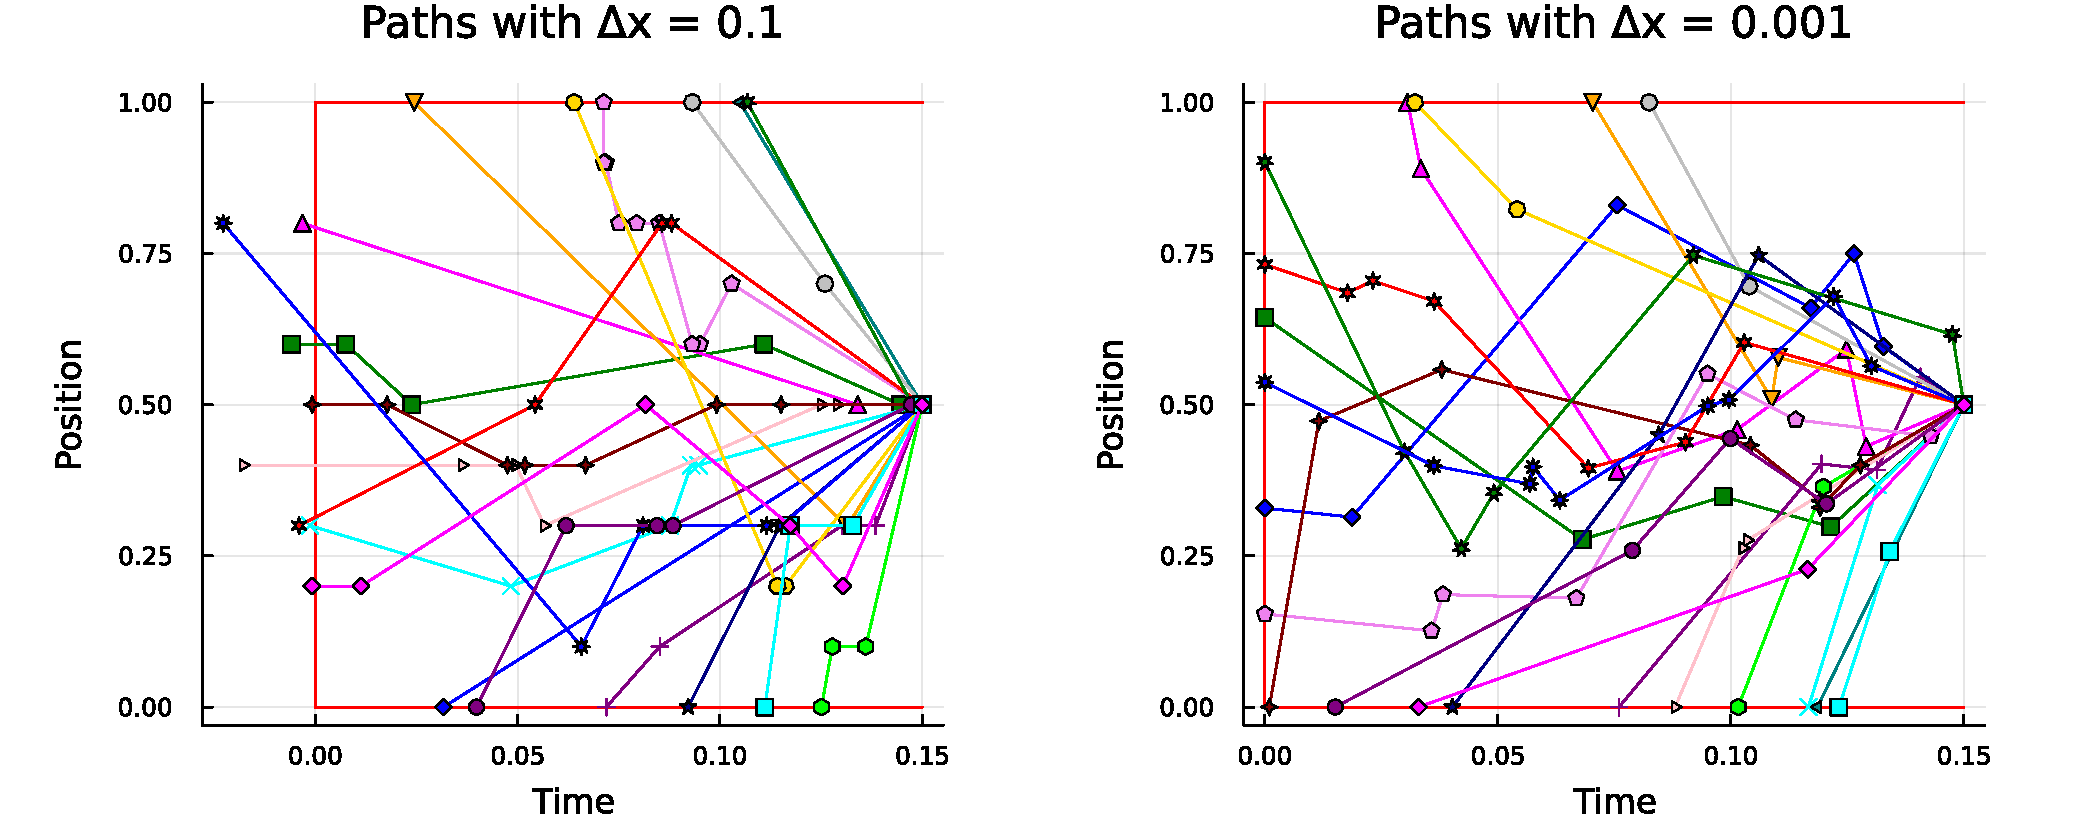
\includegraphics[width=\textwidth]{./julia_plots/paths_pest_heat_varcoef.pdf}
    \caption{$20$ samples of genPath$(x=0.5,t=0.15,dx=\{0.1,0.001\},a_{0}=0,a_{m} = 30)$. The source term is sampled
    at the intermediate points. Note that the amount of
    intermediate points does not differ much between $\Delta x = 0.1$ and $\Delta x = 0.001$.
    Points with $t<0$ do not cause any bias, the method is unbiased for the semi-discretized heat equation. }
    \label{fig:presampled paths pest heat var}
  \end{figure}

\end{technique}

\begin{julia}[\ref{jl:point estimator heat source} using precomputed paths]\label{jl:path point estimator heat source}
  We implement \ref{jl:point estimator heat source} with a precomputed path from \ref{tech:presampling heat} using tail
  recursion. Because we know the path beforehand a forward implementation is straightforward. Note that $(x,t)$ is
  never explicitly used only for figuring out how we exited the domain. The whole calculation is linear in
  $a,f$ evaluated in the source points and $u_\text{bound}$ evaluated in the exit points so there are various
  ways to optimize it for example using unbiased estimates instead of exact evaluations.

  \juliacode{julia_code/path_pest_heat_varcoef.jl}
\end{julia}




% \begin{lemma}[Brownian motion and the heat equation] \label{lem:BM HE}
%     For problem (\ref{def:heat equation}) if $ |\psi|$ is bounded
%     then there holds:

%     \begin{equation}
%         u(x,t)=E[\psi(Y_{\tau},\tau) | Y_{t} =x].
%     \end{equation}
%     With $dY_{s} = dW_{-s},\tau = \sup\{s | (Y_{s},s) \notin \Omega\}$.
% \end{lemma}


% \begin{proof} \label{proof: BM HE }
%     Discretize the heat equation
%     with a regular rectangular mesh that includes $(x,t)$ with equally
%     spaced intervals over space and time ($\Delta x, \Delta t$) with
%     the corresponding difference equation:

%     \begin{equation}
%         \frac{u(x,t)-u(x,t-\Delta t)}{\Delta t} = \frac{u(x + \Delta x,t)-2 u(x,t) +u(x - \Delta x,t)}{\Delta x^{2}} .
%     \end{equation}

%     Isolate $u(x,t)$:

%     \begin{equation} \label{eq:discrete iso heat equation}
%         u(x,t) =
%         \frac{\Delta t}{ 2 \Delta t + \Delta x^{2}}
%         \left(
%         u(x+\Delta x,t)+u(x-\Delta x,t)
%         \right) +
%         \frac{\Delta x^{2}}{ 2 \Delta t + \Delta x^{2}}
%         \left(
%         u(x,t-\Delta t)
%         \right).
%     \end{equation}

%     Because $u(x+\Delta x,t) \approx u(x-\Delta x,t) \approx u(x,t-\Delta t) \approx$
%     right-hand side of equation (\ref{eq:discrete iso heat equation}) we may Russian roulette
%     to remove branching recursion and generate a recursion path instead of a tree.
%     \begin{equation} \label{eq:RRVE discrete heat equation }
%         Z(x,t) =
%         \begin{cases}
%             \psi(\text{argmin}_{b \in \partial \Omega} ||(x,t) - b||)
%              & \text{ when } (x,t) \notin \Omega \\
%             \begin{cases}
%                 Z(x+\Delta x , t)  & \text{ with chance  } \frac{\Delta t}{ 2 \Delta t + \Delta x^{2}}     \\
%                 Z(x-\Delta x , t)  & \text{ with chance  } \frac{\Delta t}{ 2 \Delta t + \Delta x^{2}}     \\
%                 Z(x, t - \Delta t) & \text{ with chance  } \frac{\Delta x^{2}}{ 2 \Delta t + \Delta x^{2}}
%             \end{cases}
%              & \text{ else }.
%         \end{cases}
%     \end{equation}
%     This is a RRVE, $Z$ has finite variance because $ |\psi|$ is bounded
%     and $E[Z(x,t)]$ is the solution to the discretized heat equation. Taking the limit
%     makes the discrete solution converge to the real solution.
%     For (\ref{eq:RRVE discrete heat equation }) the limit
%     makes the recursion path go to Brownian motion $Y_{t}$.
%     \begin{equation}
%         Z(x,t) \rightarrow \psi(Y_{\tau},\tau)  .
%     \end{equation}
%     Finishing the proof.
% \end{proof}

% % maybe with the source

% \begin{related}
%   % (\ref{lem:BM HE}) is a subcase of the Feynman-Kac formula.
%   % For a proof and an in-depth discussion of the Feynman-Kac formula
%   % see . \\
%   The Feynman-Kac formula is related to this. See \cite{oksendal_stochastic_2003}
%   for a reference.
% \end{related}


% \begin{theorem}[Feynman-Kac formula (wikipedia)] \label{thrm:feymankac}
%     Consider the partial differential equation
%     \begin{equation}
%         \frac{\partial u}{\partial t}(x, t)+\mu(x, t) \frac{\partial u}{\partial x}(x, t)+\frac{1}{2} \sigma^2(x, t) \frac{\partial^2 u}{\partial x^2}(x, t)-V(x, t) u(x, t)+f(x, t)=0,
%     \end{equation}
%     defined for all $x \in \mathbb{R}$ and $t \in[0, T]$, subject to the terminal condition
%     \begin{equation}
%         u(x, T)=\psi(x),
%     \end{equation}
%     where $\mu, \sigma, \psi, V, f$ are known functions, $T$ is a parameter, and $u: \mathbb{R} \times[0, T] \rightarrow \mathbb{R}$ is the unknown. Then the Feynman-Kac formula tells us that the solution can be written as a conditional expectation
%     \begin{equation}
%         u(x, t)=E^Q\left[\int_t^T e^{-\int_t^r V\left(X_\tau, \tau\right) d \tau} f\left(X_r, r\right) d r+e^{-\int_t^T V\left(X_\tau, \tau\right) d \tau} \psi\left(X_T\right) \mid X_t=x\right]
%     \end{equation}
%     under the probability measure $Q$ such that $X$ is an Itô process driven by the equation
%     \begin{equation}
%         d X_t=\mu(X, t) d t+\sigma(X, t) d W_t^Q
%     \end{equation}
%     with $W^Q(t)$ is a Wiener process (also called Brownian motion) under $Q$, and the initial condition for $X(t)$ is $X(t)=x$.
% \end{theorem}

\subsection{First Passage Sampling}

In this subsection we discuss recursive first passage sampling to efficiently
first passage sample complicated geometries.


\begin{definition}[first passage time] \label{def:first passage time}
  Define the first passage time for a process $X_{t}$ for a set of valid states
  $V$ as
  \begin{equation}
    \text{FPt}(X_{t},V)=\inf \{t>0| (X_{t},t) \notin V \}
    .
  \end{equation}
  Note that the first passage time is a RV itself.
\end{definition}

\begin{definition}[first passage] \label{def:first passage}
  Define the first passage for a process $X_{t}$ for a set of valid states
  $V$ as
  \begin{equation}
    \text{FP}(X_{t},V)=(X_{\tau},\tau), \tau = \text{FPt}(X_{t},V)
    .
  \end{equation}
\end{definition}

\begin{lemma} \label{lem: FP order}
  When a process has more valid states the first passage time gets larger i.e.
  \begin{equation}
    V_{1} \subset V_{2} \Rightarrow
    \text{FPt}(X_{t}(\omega),V_{1}) \le  \text{FPt}(X_{t}(\omega),V_{2}) .
  \end{equation}
  The $\omega$ is to indicate the same realization of $X_{t}$.
\end{lemma}

\begin{theorem}[Green's functions and first passage distribution]
  The density of first passages of Code \ref{jl:point estimator heat} is the
  corresponding Dirichlet boundary Green's function for the semi-discretized heat equation.
\end{theorem}

% notation for the Green's function is bad
\begin{proof}
  Follows directly from the definition.
  Let $P(x,t|x_{0},t_{0})$ denote the boundary Green's
  function for the semi-discretized heat equation and $X_{t}$
  the corresponding space time process.
  \begin{align}
    P(x,t|x_{0},t_{0}) & = E[Y(x_0,t_0)]                                         \\
                       & = E[\tilde{u}(X_{\tau},\tau) | X_{t_0} = x_0 ]          \\
                       & = E[\delta_{((X_{\tau},\tau) = (x,t))}| X_{t_0} = x_0 ] \\
                       & = P((X_{\tau},\tau) = (x,t)| X_{t_0} = x_0 )
    .
  \end{align}
\end{proof}


Another way to obtain an unbiased estimator for the semi-discretized heat equation is using unbiased estimates
of the boundary Green's boundary function. Because of:

\begin{align}
  \tilde{u}(x_{0},t_{0}) & = \int_{\partial \Omega} \tilde{u}(x,t) P(x,t|x_{0},t_{0}) d(x,t)                    \\
                         & = \int_{\partial \Omega} \tilde{u}(x,t)  dP((X_{\tau},\tau) = (x,t)| X_{t_0} = x_0 )
  .
\end{align}

\begin{related}[recursively estimating Green's functions]
  In \cite{qi_bidirectional_2022} unbiased estimators for the boundary Green's function are constructed
  by recursively sampling known Green's functions.
\end{related}

Similar to recursively  sampling simpler Green's function we recursively sample first passages.

\begin{technique}[recursive first passage sampling]
  Recursive first passage sampling involves sampling an initial,
  simpler first passage, the base that includes fewer valid states. Using
  this sampled first passage as a starting point, we
  then perform the same sampling process until the sampled
  first passage is almost invalid.
\end{technique}

\begin{example}[Euler first passage sampling] \label{ex:euler first passage sampling}
  In this example, we approximately sample the first passage of Brownian motion
  for a parabolic barrier by simulating Brownian motion with the Euler scheme. We plotted
  this in Figure \ref{fig:Euler first passage para}. The accuracy of the sampled first passage
  are $O(\Delta t)$ and the cost to sample is $O(\Delta t ^{-1})$.

  \juliacode{julia_code/sample_euler_triangle.jl}
  \begin{figure}[h!]
    \centering
    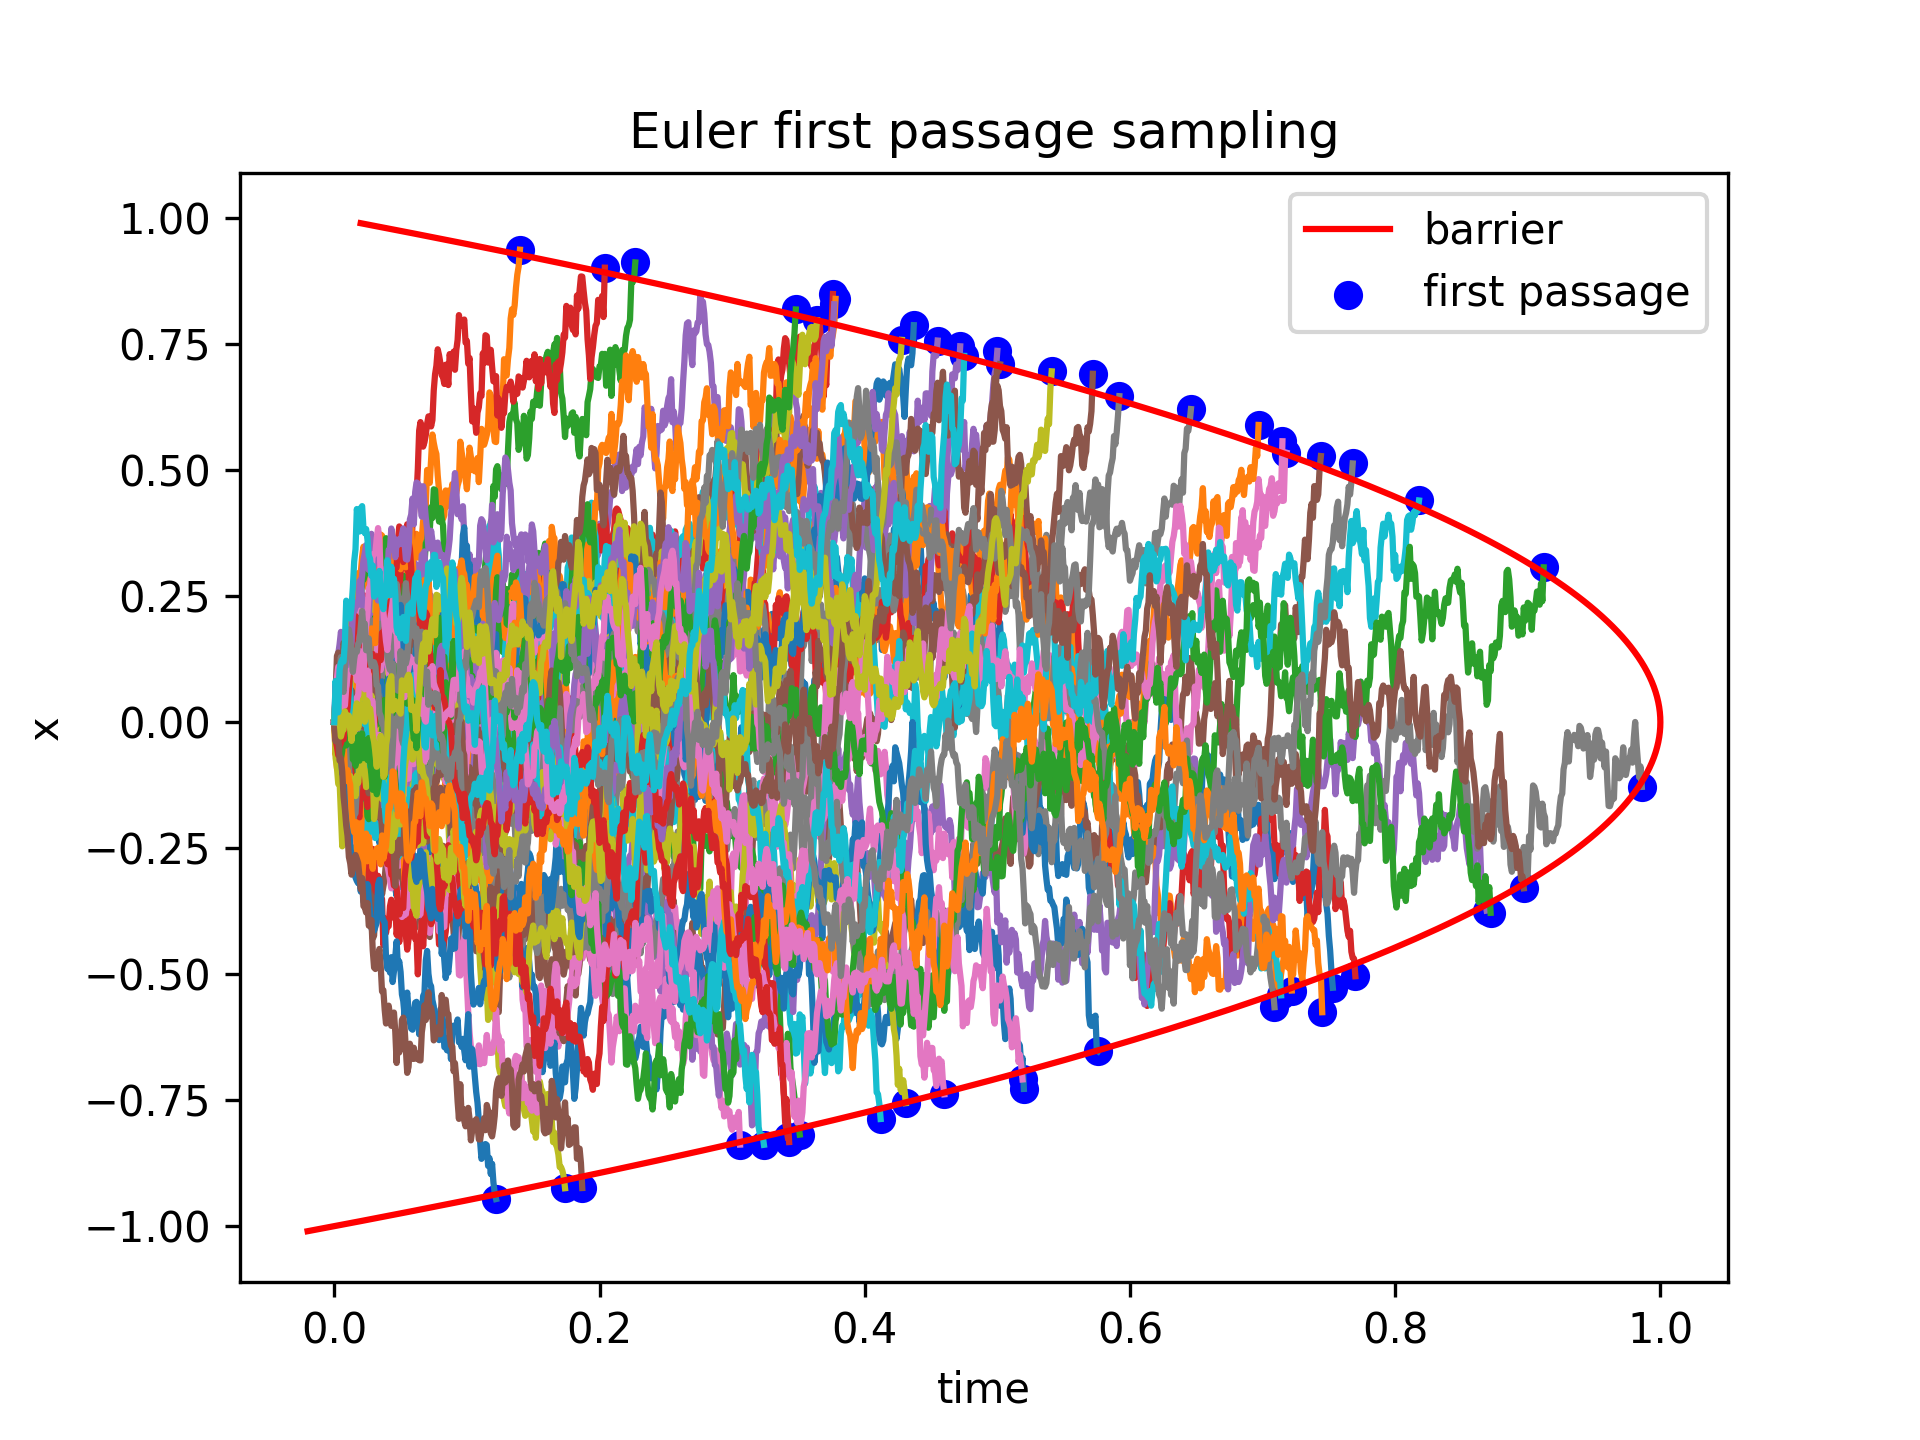
\includegraphics[width=0.8\textwidth]{plots/Euler_first_passage_para.png}
    \caption{ $50$ realizations of Euler first passage sampling with step size $0.001$.}
    \label{fig:Euler first passage para}
  \end{figure}
\end{example}


\begin{example}[recursive first passage sampling] \label{ex:recursive first passage sampling}
  In this example, we sample the first passage of Brownian motion from a parabolic barrier
  with recursive first passage sampling.
  For the simpler first passage sampler, we  exploit the self-affinity of Brownian motion
  ($\frac{W_{ct}}{\sqrt{c}} \sim W_{t}$)
  by scaling and translating
  samples from a triangular barrier so its
  valid states are contained in the parabola generated
  by the Euler scheme. The precomputed samples are created
  by \ref{ex:euler first passage sampling}.
  Assuming that the error of the base sampler is insignificant.
  The accuracy of the sampled first passage
  are $O(\varepsilon)$ and the cost to sample is $O(\ln \left(\varepsilon^{-1}\right))$.
  Note that resampling with replacement produces dependent samples and introduces additional error.
  For MC applications dependence is not an issue and when the additional error is significant resampling
  without replacement can be used.

  \juliacode{julia_code/sample_recu_para.jl}
  When the domain is convex, the maximum scaling of the triangular barrier that fits
  is easier to obtain.
  To dampen barrier
  overstepping of \ref{ex:euler first passage sampling} we use a smaller scaling
  than the maximum.

  \begin{figure}[h!]
    \centering
    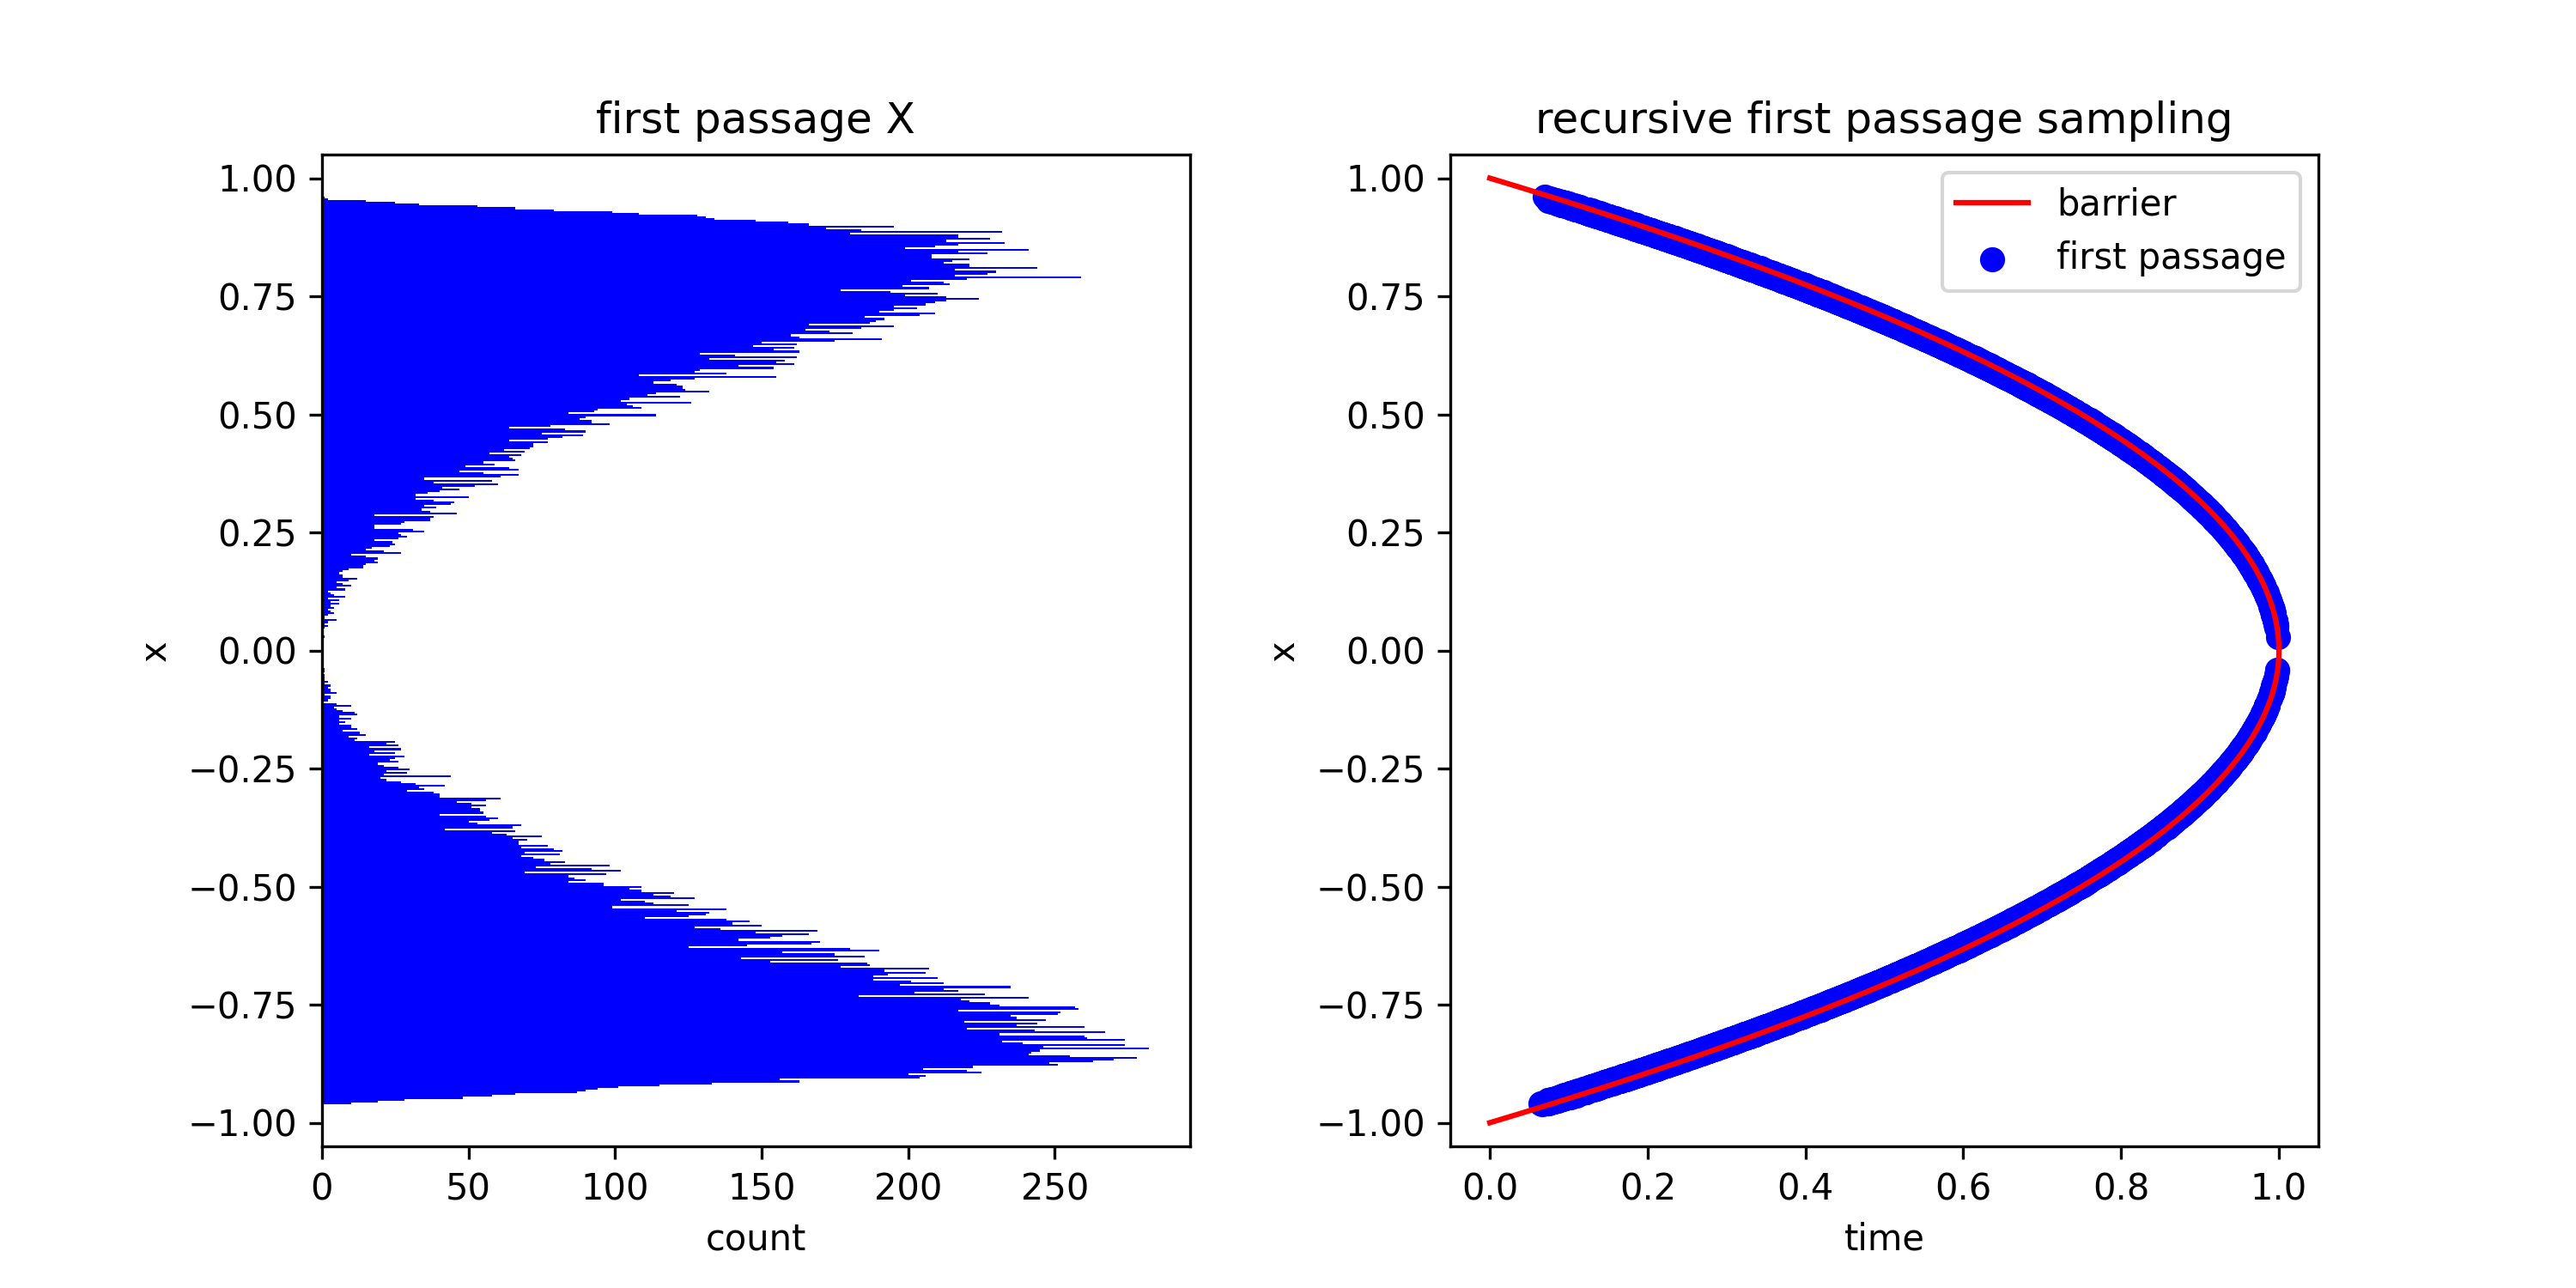
\includegraphics[width=1\textwidth]{plots/recursive_first_passage_para.png}
    \caption{ $50000$ of realizations of recursive first passage sampling produced
      by (\ref{ex:recursive first passage sampling}). The precomputed sample of $5000$ first
      passages of a triangular barrier uses the Euler scheme with
      step size $0.001$.}
    \label{fig:recursive first passage para}
  \end{figure}

\end{example}

% \begin{pythonn}[Euler first passage sampling] \label{py:euler FP sampling}
%     \pythoncode{python code/sample_euler_triangle.py}
% \end{pythonn}

% \begin{pythonn}[recursive first passage sampling] \label{py:recu FP sampling}
%     The maximum scaling of the triangular barrier that fits
%     in the parabola is derived through (\ref{lem:self affine})
%     and using the fact that a parabola domain is convex. To dampen barrier
%     overstepping of (\ref{py:euler FP sampling}) we use a smaller scaling
%     than the maximum. \\
%     \pythoncode{python code/sample_recu_para.py}

%     \begin{figure}[h!]
%         \centering
%         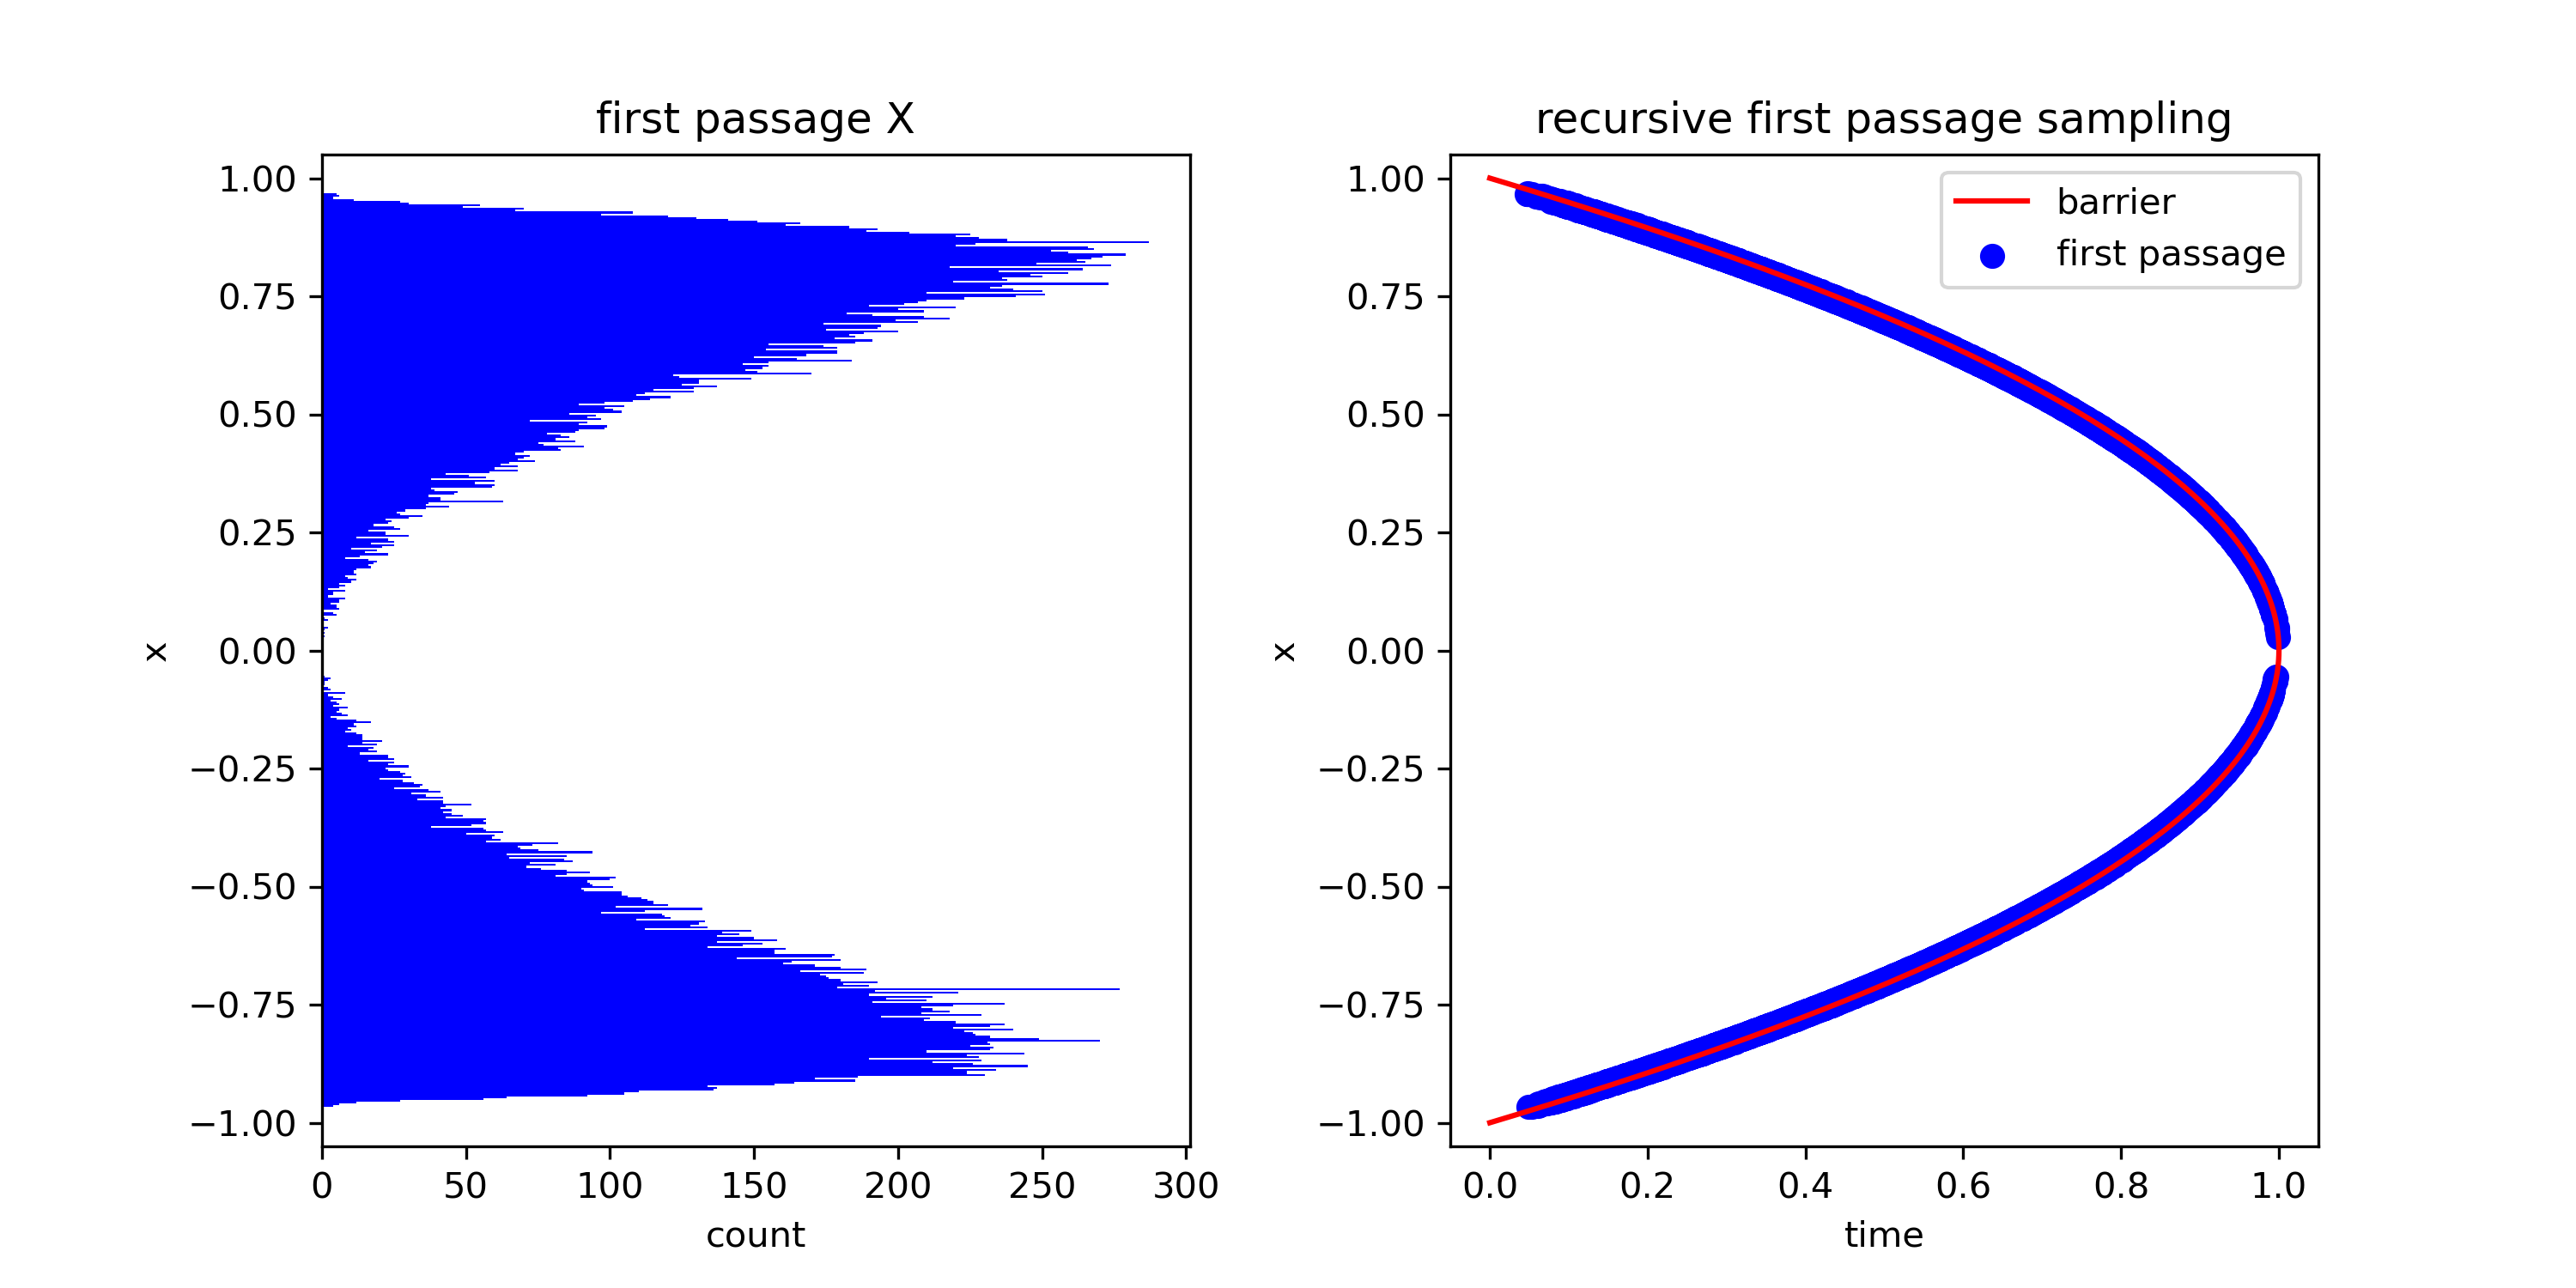
\includegraphics[width=1\textwidth]{plots/recursive first passage para.png}
%         \caption{ $50000$ of realizations of recursive first passage sampling produced
%             by (\ref{py:recu FP sampling}). The precomputed sample of $5000$ first
%             passages of a triangular barrier uses the Euler scheme with
%             step size $0.001$.}
%         \label{fig:recursive first passage para}
%     \end{figure}
% \end{pythonn}

\begin{related}[recursive first passage sampling]
  The original walk on spheres is a recursive first passage algorithm.
  Recursive first passage sampling for
  Brownian motion is discussed in \cite{herrmann_first-passage_2016}
  and by transformation also first passage problems for the
  Ornstein-Uhlenbeck process.
  % To add jumps you can use \cite{herrmann_exact_2021}.
  A more efficient alternative to resampling from an Euler scheme is to use tabulated
  inverse cumulative probability functions,
  as demonstrated in \cite{hwang_simulationtabulation_2001}.
\end{related}

% For recursive first passage sampling for high dimensional Brownian motion
% there symmetry trick to be pulled off


% \begin{example}[recursive first passage average sampling] \label{ex:recu FP average}
%     In example (\ref{ex:recursive first passage sampling}) it is possible to keep
%     track of the average because it scales and translates with our base first passage sampler.

%     \begin{figure}[h!]
%         \centering
%         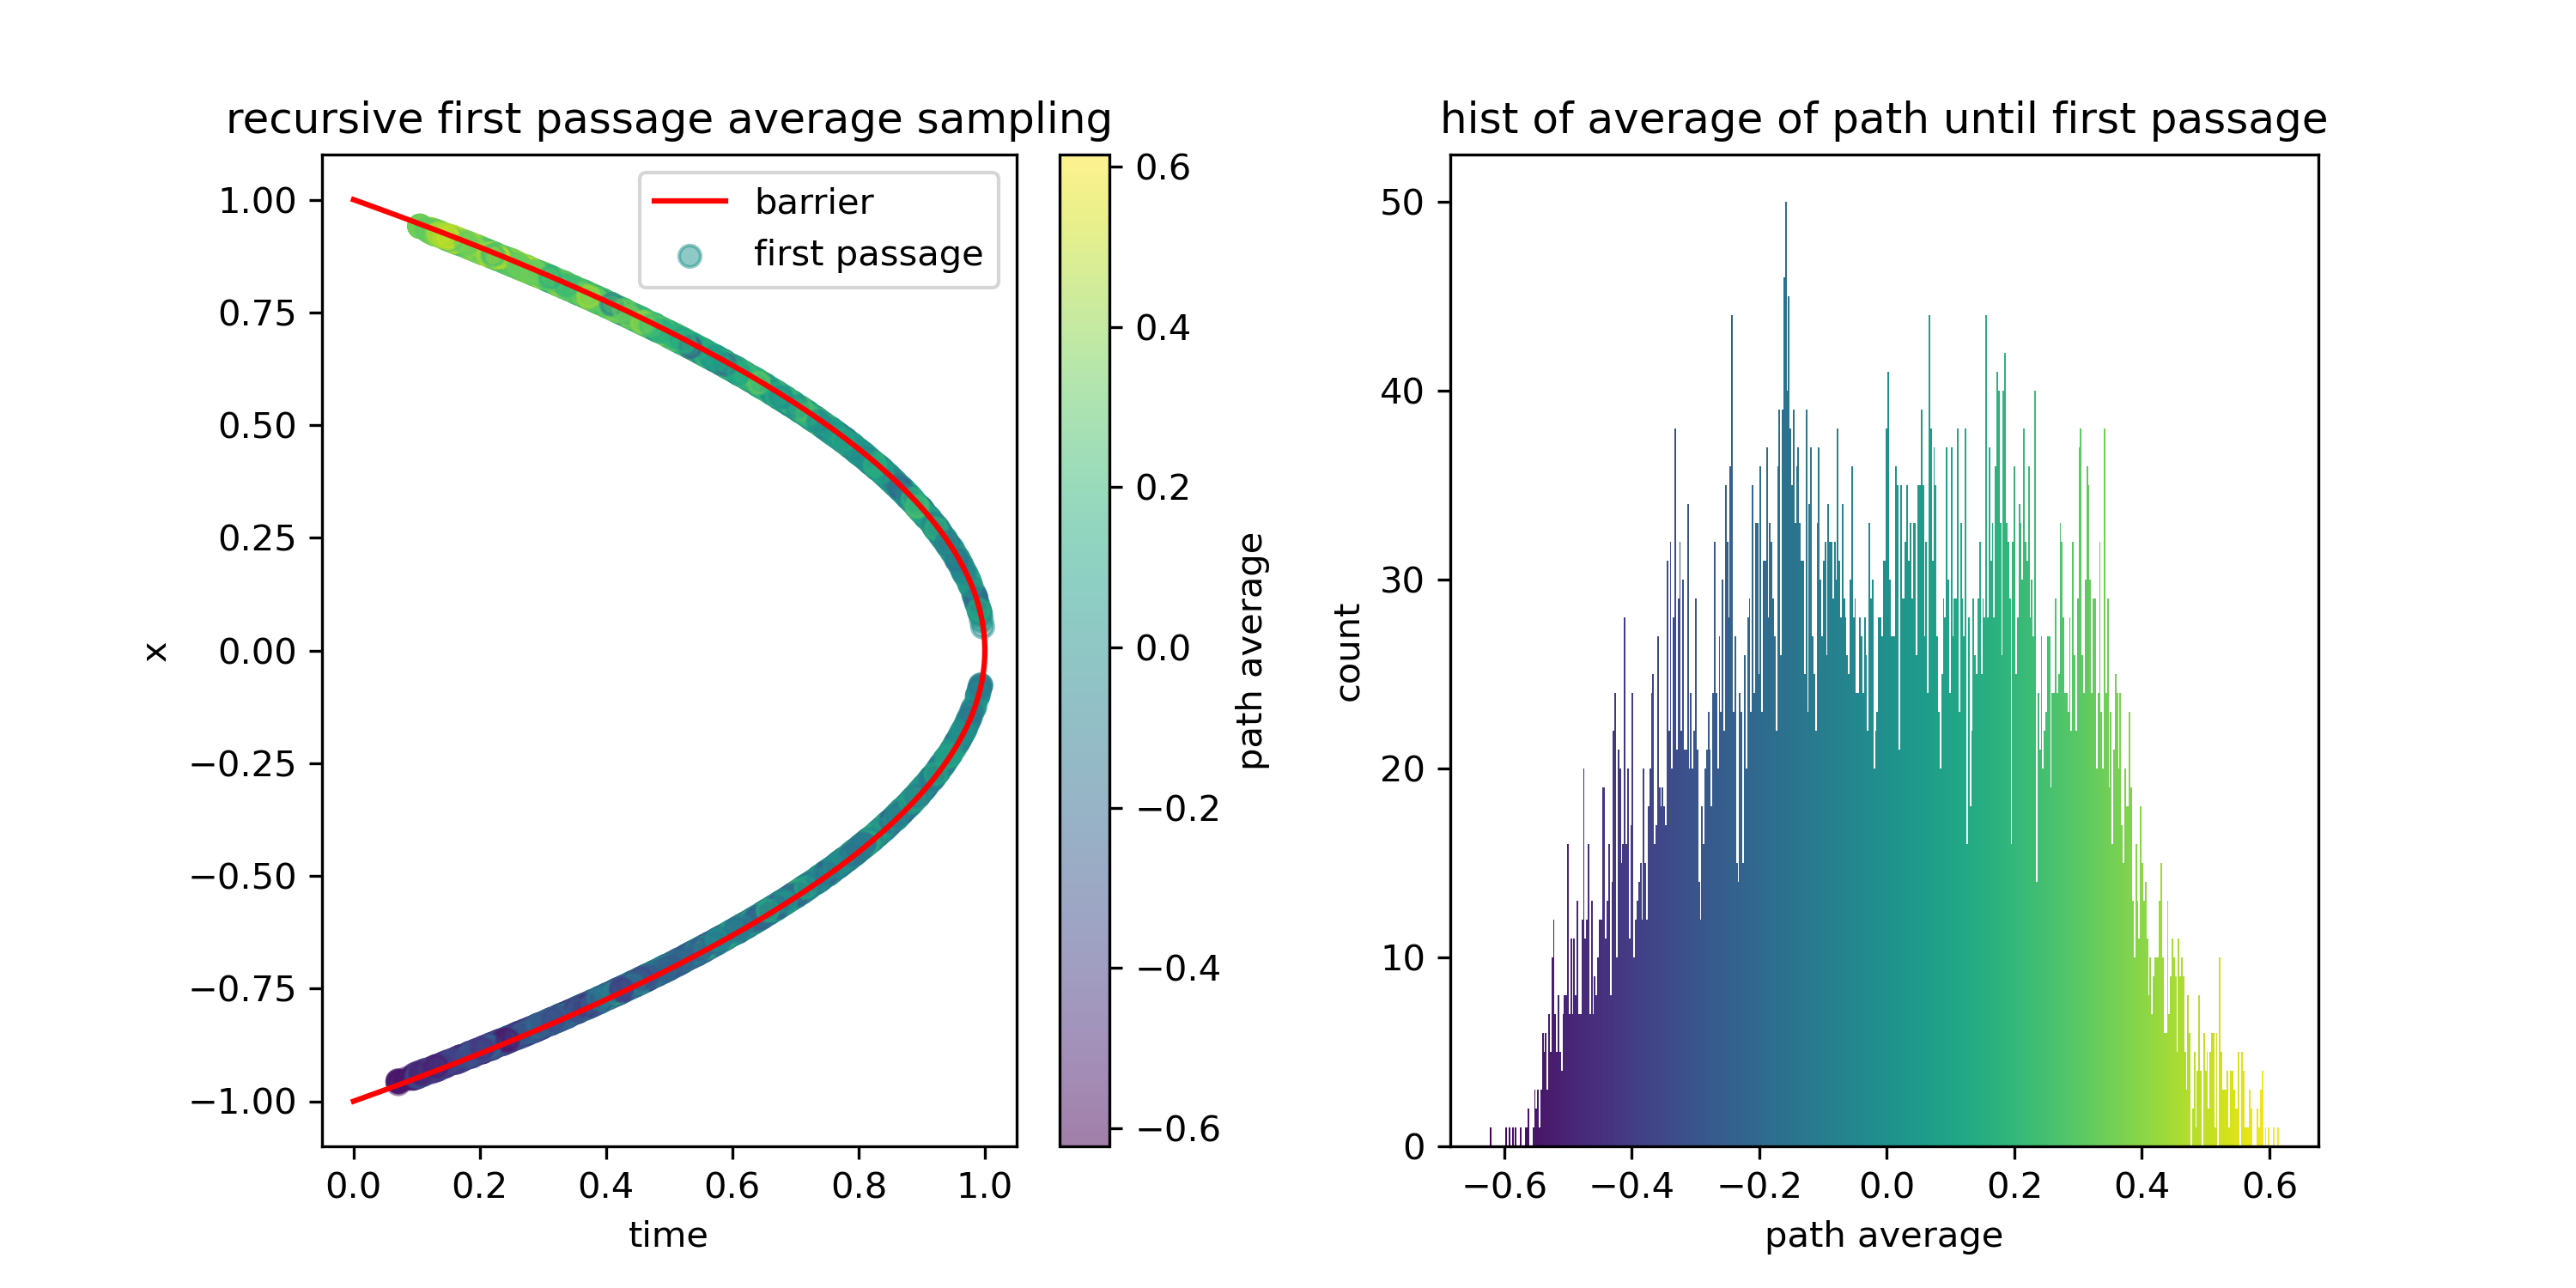
\includegraphics[width=1\textwidth]{plots/recursive first passage average para.png}
%         \caption{ $10000$ of realizations of recursive first passage sampling (for the average).
%             The precomputed sample of $1000$ first passages and averages of a triangular barrier
%             uses the Euler scheme with step size $0.001$.}
%         \label{fig:recursive first passage average para}
%     \end{figure}
% \end{example}


\begin{technique}[Brownian motion path stitching]
  Sampling approximate Brownian motion paths also can be
  framed as a first passage problem. Instead of sampling
  first passage points we sample first passage paths.
  This requires a simple first passage paths sampler and the paths
  sampled this way are "stitched" together.
\end{technique}

\begin{example}[path stitching parabola]
  Example \ref{ex:recursive first passage sampling} but
  resampling full Euler scheme generated paths.
  The advantages over generating paths directly from
  the Euler scheme are that computations for all small steps from the
  base sampler are avoided and the full path
  can be represented by its subpaths and their scalings
  requiring less memory than a fully stored path.
  The only downsides are correlation between paths and
  inhomogeneous time steps.

  \begin{figure}[h!]
    \centering
    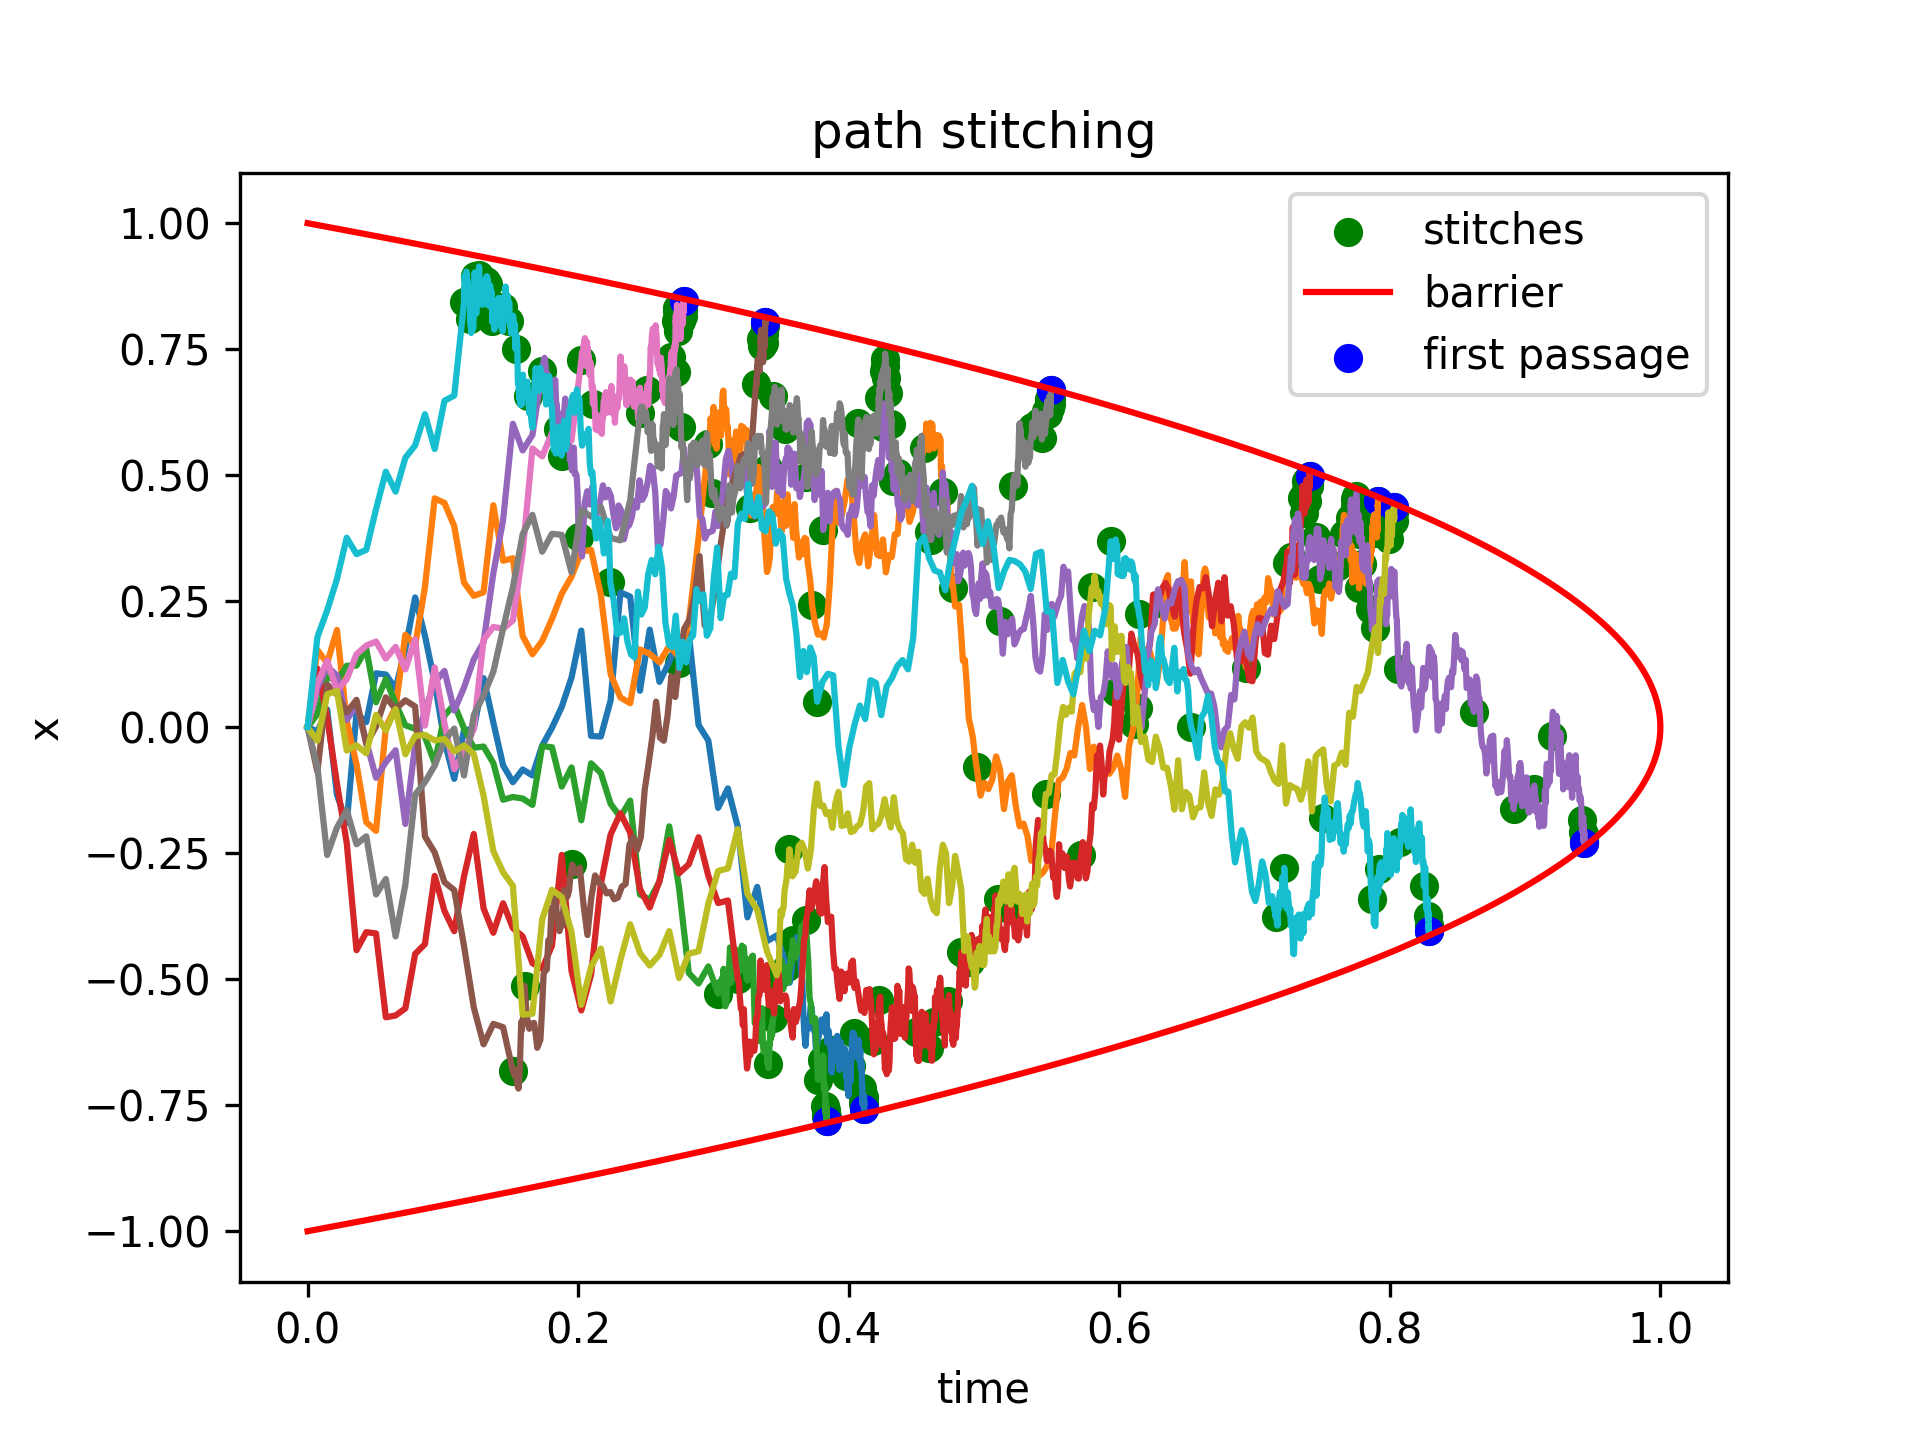
\includegraphics[width=0.8\textwidth]{plots/path_stitching_para.png}
    \caption{ $10$ paths build with path stitching build out of
      resampled Euler scheme generated paths with step size $0.01$.}
    \label{fig:path stitching para}
  \end{figure}
\end{example}

% For plotting the path we needed to accesses to all of its points.  

% A way around scaling base samples is limiting scaling to a
% discrete set and pick the biggest scaling that fits, instead
% of generating base samples for $1$ scale and scaling it dynamically
% precompute all the discrete scalings. \\


\begin{related}[path stitching]
  Path stitching appears frequently in rendering and also in \cite{das_sarma_fast_2015}
  and \cite{ji_reusing_2012}.
\end{related}

% \subsection{Limitations and Future Work}

% It would be interesting to extend proof technique of (\ref{lem:BM HE}) to the full
% Feynman-Kac formula. Just adding a source term $f$ in the Feynman-Kac formula adds
% an integral of the source term over the recursion path.
% In equation (\ref{eq:discrete iso heat equation})
% it would add $\frac{\Delta t \Delta x^{2}}{2 \Delta t + \Delta x ^{2}} f(x,t)$
% term. This term can either be kept or Russian rouletted
% to prevent infinite source evaluations in the limit.
% This roughly corresponds to estimating the integral by
% MC integration also requires knowing a finite amount of
% intermediate points of the recursion path
% sampled randomly. These can possibly be obtained from
% the intermediate first passages of recursive first passage sampling or with a smart
% application of path stitching. \\


% Recursive first passage sampling for Brownian motion can be extended to geometric
% Brownian motion by transforming the space. However, this transformation breaks
% the symmetries required for the average used in the example (\ref{ex:recu FP average}).
% An unsatisfying way to fix this is to approximate the base sampler at different points in
% space and at different scales. Just accelerating a classic Euler scheme at critical places
% with a base sampler can reduce precomputation requirements.


\section{Limitations and Future Work}

We believe that understanding and optimizing unbiased and deterministic linear ODE solvers
is the key to developing better randomized ODE/PDE solvers.
Randomized ODE/PDE solvers are useful for cases with little structure
where the advantage of IBC is significant or where the linear trade-off
between cost and variance is close to optimal. \\


Besides that, some problems require access to low-bias solutions of
ODEs. For example, when integrating a high-dimensional parametric ODE problem.
The following example is a toy problem to showcase this.

\begin{example} \label{ex:random ode}
  Consider the following parametric IVP:
  \begin{equation}\label{eq:random ode}
    y_t = ay, \quad y(0)=1,
  \end{equation}
  with $a$ a parameter. The solution to this problem is given by
  $y(t,a) = e^{ta}$. Imagine we have a belief about $a$ quantized
  in the following way $a\sim U$. If we want
  to estimate $E[y(t, U)]$ or in a more general case
  $E[f(y(t, U))]$ with $f$ analytic directly
  we need samples of $y(t,U)$. If we don't have a solution for the parametric IVP
  we can't sample $y(t,U)$ instead, we use unbiased estimates ($Y(t,u)$) of samples ($y(t,u)$)
  of $y(t, U)$ in the following
  way using the total law of expectation:

  \begin{align}
    E[f(y(t,U))] & = E[f(y(t,u)) \mid U=u]     \\
                 & = E[f(E[Y(t,u)]) \mid U=u].
  \end{align}

  To estimate $E[f(E[Y(t,u)]) \mid U =u]$, we use the approach outlined in
  Example \ref{ex:exp int}. The first two moments of $y(t, U)$ are:
  \begin{align}
    E[y(t,U)]      & = \frac{e^t}{t} - \frac{1}{t},      \\
    E[y^{2}(t, U)] & = \frac{e^{2t}}{2t} - \frac{1}{2t}.
  \end{align}
\end{example}

\begin{pythonn}[implementation of Example \ref{ex:random ode}]
  \pythoncode{python code/random_ODE.py}
\end{pythonn}

\vspace{0.5cm}

The time process we used based on Example \ref{ex: russian roulette}
has little control over the distribution of recursion calls $(t,Y(t))$
in time see Figure \ref{fig:russian roulette}.

\begin{figure}[h!]
  \centering
  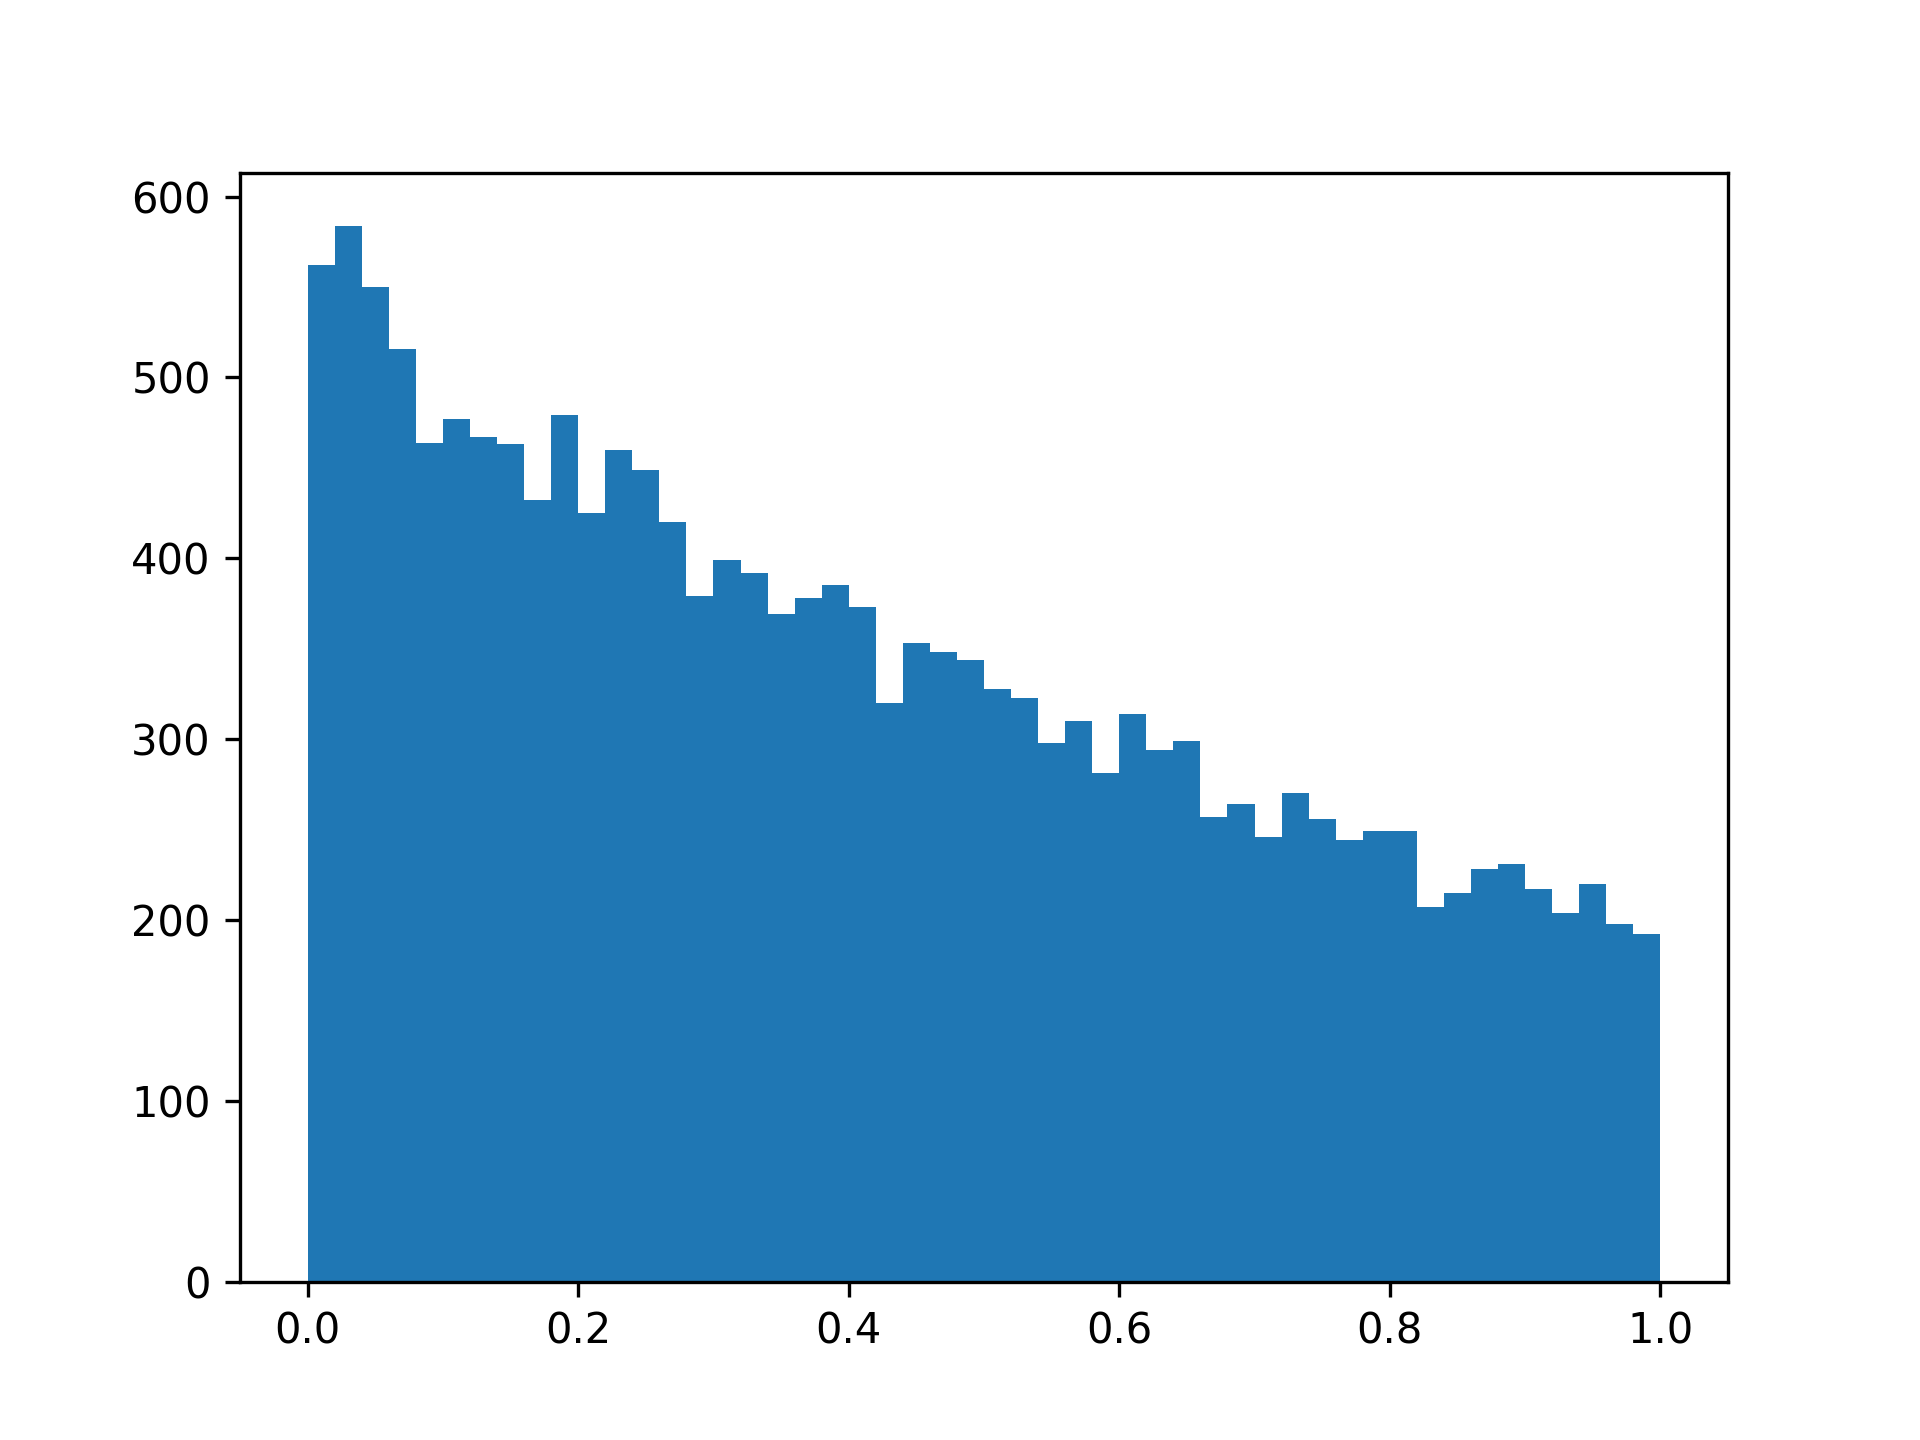
\includegraphics[width=0.8\textwidth]{plots/time process.png}
  \caption{This histogram depicts how the points
    on Figure \ref{fig:russian roulette} are distributed over time
    excluding $t=1$.}
  \label{fig:time proces}
\end{figure}

Instead of that, a Poisson point process can be used.
It samples backward with the corresponding
exponential distribution and employs Russian roulette
when out of range. The distribution of the recursion calls over time
can be controlled by its intensity.
In the case of constant intensity, the number of recursive calls
follows a Poisson distribution. \\

Besides the time process, other areas of development could
include the cheaper construction of control variates,
different types of control variates, adaptive schemes,
freezing less important terms in the inner recursion or Russian rouletting
them into reasonable approximations, error estimates based on variance in the
inner recursion, etc. \\

To handle stiff problems we weigh towards exponential integrators
type of methods. The biggest obstacle to implementing them similar to diagonal RRMC
is getting unbiased estimates of $e^{A(t-s)} y(s)$ type of expressions. In the case
of a big matrix $A$  unbiased sparsifaction will probably be useful
see \cite{sabelfeld_sparsified_2009}.
Initially, we came up with Example \ref{ex:exp int}, but some time later,
we found the paper from NVIDIA \cite{kettunen_unbiased_2021} that optimizes
that example. Closely related to this is directly estimating the Magnus expansion,
where expressions like $e^{\int_{0}^{\Delta t} A(s)ds} y(0)$ are needed.
In this case, \cite{kettunen_unbiased_2021} doesn't utilize the smoothness of
$A(s)$, which is necessary
for optimal IBC.

One of the elements lacking in our findings is rigor.  We believe
that RMC is an informal approach to an unbiased estimate of
the Von Neumann series to the corresponding integral equation.
\cite{ermakov_monte_2021} presents Theorems $1$ and $2$ to
show that their estimates have finite variance and provide an expression for it.
Before becoming aware of \cite{ermakov_monte_2021}, we
previously derived a similar expression (with errors)
by employing the law of total variance, similar to (16) in \cite{rath_ears_2022}. \\
We believe that proving the optimality of IBC in Example \ref{ex:CV RRMC IVP} is feasible
but tedious.
\cite{daun_randomized_2011} presented a proof for optimal IBC for their algorithm.
The proof we have in mind is using a lower bound on IBC
from integration and proving it is attained.\\

Optimal IBC isn't everything. Being optimal in IBC doesn't necessarily mean it's optimized.
An algorithm that uses $1000$ times more function calls may still have the same
IBC. Additionally, the computational goal
might not align well with the IBC framework.
We admire \cite{becker_learning_2022},
which employs deep learning to extend beyond the IBC framework.
The emphasis here is on performing multiple rapid solves (inferences)
while allowing for an expensive precomputation (training).
IBC also doesn't take into account the parallel nature of computations.
Given infinite parallel resources, it would be reasonable to cease reducing
variance by decreasing the step size and instead opt for splitting the final estimator.
The only necessary communication in splitting is averaging the final
estimator. We hypothesize that for RMC, the wall time at risk
increases logarithmically with the size of the splitting.



\newpage
\begin{abstract}
  Deze scriptie onderzoekt unbiased Monte Carlo methoden voor
het oplossen van lineaire gewone differentiaalvergelijkingen met het
oog op partiële differentiaalvergelijkingen.
De voorgestelde algoritmes maken gebruik van de geschikte
combinatie van Monte Carlo technieken. Deze Monte Carlo technieken
worden geïntroduceerd met voorbeelden en code.
\end{abstract}

\printbibliography
\newpage

\end{document}

% Base your answers on the thesis.  
% You are expert in solving ODEs, WoS, IBC, PDEs giving feedback.
%
% Answer as a markdown file.
% Use subnumerings in mark down form in numbering the question 
% that works in a markdown file and use different headers. Like this: 
%
% # Content tests
% ##  0.1. How does the main algorithm work of the thesis?
% answer
%
% Here are the questions : 
% # Content tests
% 0.1. How does the main algorithm work of the thesis?
% 0.2. What is the biggest limitation of the main algorithm of the thesis?
% 0.3. How important is coupled splitting to the thesis?
% 0.4. How does Stein's paradox pop up in the thesis? (see subsection on MC integration)
% 0.5. Rate the language of the thesis.
% 0.6. List the 5 unclearest parts of the thesis.
% 0.7. What is special about the Monte Carlo trapezoidal rule?
% 0.8. What is the main advantage of the primary motivating work? 
% 0.9.  How does the thesis define Russian Roulette?
% 0.10. How does the thesis define control variates?
% 0.11. Summarize the approach for exponential of the expectance in the unbiased non-linearity section.
% 0.12. How does the thesis define tail recursion?
% 0.13. How does the thesis define Green's functions? 
% 0.14. Summarize convergence behavior of the main algorithm.
% 0.15. List your 5 favorite/intrestring parts of the thesis.
% 0.16. What seem to be missing in the thesis?
% 0.17. Any abbreviation that should/shouldn't be used?
% 0.18. List 5 inaccuracies things in the thesis.
% 0.19. List 5 controversial things in the thesis.
% 0.20. List 5 suggestions to improve the thesis.
%
% # Feedback 1
% 1.1 Does the thesis differentiate between the original contributions and prior work? 
% 1.2 Does the thesis has a good overview?
% 1.3 Does the thesis has a good conclusion?
% 1.4 Does everything gets defined in the thesis?
% 1.5 Are there symbols that don't get defined in the thesis?
% 1.6 What are the advantages of the solvers in the subsection of initial value problems 
% compared to classical solver?
% 1.7 Are the explanations for the graphs in the thesis sufficient?
% 1.8 Do equations, examples, definition, etc get referenced with consistent notation?
% 1.9 List 2 uncommon abbreviations that don't get introduced the first time they get used. 
%
% # Feedback 2
% 2.1 Has the elementary theory of Monte Carlo been covered in the thesis?
% 2.2 In the subsection of recursive Monte Carlo why is there indefinite 
% recursion?
% 2.3 Does the thesis give the necessary references to concepts?
% 2.4 Does additive branching gets explained clearly?
% 2.5 What is the Russian roulette rate ?
% 2.6 Does the local truncation error get defined ?

% # Requirements
% 3.1 Title Page: Does the thesis have a title page? 
% 3.2 Table of Contents: Does the thesis include a table of contents?
% 3.3 Introduction: 
%     Does the introduction provide a clear context for the research?
%     Is the problem statement or research question clearly formulated in the introduction?

% 3.4 Exposition:
%     Is the argumentation detailed and logical, leading to the final result of the research?
%     Is the substructure effectively used to organize and clarify the content within the exposition?

% 3.5 Dutch Summary:

%     Does the thesis include a Dutch summary?
%     Is the Dutch summary concise, effectively summarizing the main points of the thesis within the specified page limit?

% 3.6 Bibliography:

%     Is the bibliography section present and well-structured?
%     Are all the cited sources accurately listed in the bibliography according to the specified citation style?

% 3.7 Layout and Readability:
%   - Is the layout designed to enhance readability, including appropriate font, line spacing, and paragraph structure?
%   -  Is the use of headings, subheadings, and other formatting elements consistent and effective in guiding the reader through the content?

% 3.8 Language Quality:
% - Is the language used throughout the thesis refined and well-crafted?
% - Are grammar, spelling, and punctuation accurate?

% 3.9 Results and Analysis:

% - Are the results presented clearly and comprehensively?
% - Is the analysis of the results thorough, and do the conclusions logically follow from the data?

% 3.10 Argumentation and Coherence:

% - Is there a clear and logical progression of ideas throughout the thesis?
% - Do transitions between sections and paragraphs enhance the overall coherence of the document?

% 3.11 Original Contribution:
% - Does the thesis make a unique and valuable contribution to the field of study?
% - Is there a clear statement about how the research fills a gap in existing knowledge?

% 3.12 Discussion and Implications:
% - Does the discussion section provide insights into the broader implications of the research findings?
% - Are any practical applications or future research directions suggested?

% 3.13 Clarity and Conciseness:
% - Is the writing style clear and concise, avoiding unnecessary jargon?
% - Are complex concepts explained in a way that is understandable to the intended audience?

% 3.14 Overall Contribution:
% - Does the thesis contribute significantly to the field's body of knowledge and understanding?
% - Is the thesis likely to be cited and referenced by others in the field?

